\documentclass[11pt]{article}
\usepackage{thumbpdf,lmodern}
\usepackage[utf8]{inputenc}
%\usepackage[margin=3.3cm]{geometry}
%\renewcommand{\familydefault}{\sfdefault}
%\usepackage[top=2.5cm, left=2.8cm, right=2.8cm, bottom=2.5cm]{geometry}
\usepackage[margin=3cm]{geometry}

%%% PACKAGES
\usepackage[dvipsnames]{xcolor}
\usepackage{graphicx} % support the \includegraphics command and options
\usepackage{booktabs} % for much better looking tables
\usepackage{array} % for better arrays (eg matrices) in maths
\usepackage{paralist} % very flexible & customisable lists (eg. enumerate/itemize, etc.)
\usepackage{verbatim} % adds environment for commenting out blocks of text & for better verbatim
\usepackage{tikz}
\usepackage[all]{xy}
\usepackage{mathtools}
\usepackage{url}
\def\UrlBreaks{\do\/\do-} % this is for lineabreaking of bibliography urls
\usepackage{hyperref}
\usepackage{color}
\usepackage{float}
\usepackage[justification=centering]{caption}
\usepackage{subcaption}
\usepackage{booktabs}
\usepackage{acro}
\usepackage{setspace}
\usepackage{eurosym}
\usepackage{listings} %% for R Code
\usepackage{natbib}
%\usepackage{csquotes}
%\usepackage{footnote}
\usepackage{amsmath}
\usepackage{amsfonts}
\usepackage{amsthm}
\usepackage{courier}
\usepackage{appendix}
\usepackage{listings}


%%% Listings options
\lstdefinelanguage{Renhanced}[]{R}{
  otherkeywords={!,!=,~,\$,*,\&,\%/\%,\%*\%,\%\%,<-,<<-, ::},
  morekeywords={},
  deletekeywords={hist, runif, plot, read.table, read, check, text, file, attributes, quote, missing, c, list, any, which, na, deparse, structure, install, model, data, sub, family},
  alsoletter={.\%},%
  alsoother={:_\$}}

 \lstset{
  language=Renhanced,                     % the language of the code
  basicstyle=\small\ttfamily, % the size of the fonts that are used for the code
  numbers=left,                   % where to put the line-numbers
  numberstyle=\tiny\color{Blue},  % the style that is used for the line-numbers
  stepnumber=1,                   % the step between two line-numbers. If it is 1, each line will be numbered
  numbersep=10pt,                  % how far the line-numbers are from the code
  backgroundcolor=\color{white},  % choose the background color. You must add \usepackage{color}
  showspaces=false,               % show spaces adding particular underscores
  showstringspaces=false,         % underline spaces within strings
  showtabs=false,                 % show tabs within strings adding particular underscores
  frame=false,                   % adds a frame around the code
  rulecolor=\color{black},        % if not set, the frame-color may be changed on line-breaks within not-black text (e.g. commens (green here))
  tabsize=2,                      % sets default tabsize to 2 spaces
  captionpos=b,                   % sets the caption-position to bottom
  breaklines=true,                % sets automatic line breaking
  breakatwhitespace=false,        % sets if automatic breaks should only happen at whitespace
  keywordstyle=\color{RoyalBlue},      % keyword style
  commentstyle=\color{YellowGreen},   % comment style
  stringstyle=\color{ForestGreen}      % string literal style
}



%%% BibTex Style
\setcitestyle{authoryear, open = { ( }, close = { ) }}
\def\bibfont{\small} % smaller bibliography

% Equation numbering
\numberwithin{equation}{section}

% French spacing
\frenchspacing



\renewcommand{\lstlistingname}{Code-Chunk}

%%% New commands
\newcommand{\li}{\lstinline}
\newcommand{\estf}{\hat{\boldsymbol{f}}}
\newcommand{\estbbeta}{\hat{\boldsymbol{\beta}}}
\newcommand{\bbeta}{\boldsymbol{\beta}}
\newcommand{\by}{\mathbf{y}}
\newcommand{\bx}{\mathbf{X}}
\newcommand{\btau}{\boldsymbol{\tau}}
\newcommand{\balpha}{\boldsymbol{\alpha}}
\newcommand{\xib}{\mathbf{x}_{i}' \bbeta}
\newcommand{\btheta}{\boldsymbol{\theta}}
\newcommand{\boldeta}{\boldsymbol{\eta}}
\newcommand{\XB}{\mathbf{X} \boldsymbol{\beta}}
\newcommand{\bgamma}{\boldsymbol{\gamma}}



%%% HEADERS & FOOTERS
\usepackage{fancyhdr} % This should be set AFTER setting up the page geometry
\pagestyle{fancy} % options: empty , plain , fancy
\renewcommand{\headrulewidth}{0pt} % customise the layout...
\lhead{}\chead{}\rhead{}
\lfoot{}\cfoot{\thepage}\rfoot{}



%%% SECTION TITLE APPEARANCE
% (This matches ConTeXt defaults)

%%% ToC (table of contents) APPEARANCE
\usepackage[nottoc,notlof,notlot]{tocbibind} % Put the bibliography in the ToC
\usepackage[titles]{tocloft} % Alter the style of the Table of Contents
\renewcommand{\cftsecfont}{\rmfamily\mdseries\upshape}
\renewcommand{\cftsecpagefont}{\rmfamily\mdseries\upshape} % No bold!

\usepackage{setspace}
\onehalfspacing

%for todos
\usepackage{xcolor}
\newcommand\todos[1]{\textcolor{red}{#1}}

%\renewcommand{\arraystretch}{0.85}
\title{Master Thesis}
\author{Friederike Becker}

%%% Abbreviations
\DeclareAcronym{am}{
  short = AM,
  long  = Additive Models
}
\DeclareAcronym{gamlss}{
  short = GAMLSS,
  long  = {Generalized Additive Models for Location, Scale and Shape}
}
\DeclareAcronym{bamlss}{
  short = BAMLSS,
  long  = {Bayesian Additive Models for Location, Scale and Shape}
}
\DeclareAcronym{glm}{
  short = GLM,
  long  = {Generalized Linear Models}
}
\DeclareAcronym{ols}{short = OLS, long  = {Ordinary Least Squares}}
\DeclareAcronym{ecdc}{short = ECDC, long = {European Center for Disease Prevention and Control}}
\DeclareAcronym{gam}{short = GAM, long  = {Generalized Additive Models}}
\DeclareAcronym{star}{short = STAR, long  = {Structured Additive Regression}}
\DeclareAcronym{wls}{short = WLS, long  = {Weighted Least Squares}}
\DeclareAcronym{irls}{short = IRLS, long  = {Iteratively Reweighted Least Squares}}
\DeclareAcronym{rs}{short = RS, long  = {Rigby and Stasinopoulos}}
\DeclareAcronym{cg}{short = CG, long  = {Cole and Green}}
\DeclareAcronym{mcmc}{short = mcmc, long  = {Markov Chain Monte Carlo}}
\DeclareAcronym{iid}{short = i.i.d., long  = {independent and identically distributed}}
\DeclareAcronym{cdf}{short = cdf, long  = {cumulative distribution function}}
\DeclareAcronym{pdf}{short = pdf, long  = {probability density function}}
\DeclareAcronym{wis}{
  short = WIS,
  long  = {weighted interval score}
}

\DeclareAcronym{crps}{
  short = CRPS,
  long  = {continuous ranked probability score}
}

\usepackage{array,multirow,graphicx}

\begin{document}



%----------------------------------------------------------------------------------------
%	HEADING TITLE AND OTHER STUFF
%----------------------------------------------------------------------------------------

%\textsc{Georg-August Universität Göttingen}\\[1.5cm] % Name of your university/college
\newgeometry{top = 3cm, left = 2.5cm, right = 2.5cm}
\pagenumbering{Alph}
\begin{titlepage}
\thispagestyle{empty}
\newcommand{\HRule}{\rule{\linewidth}{0.6mm}} % Defines a new command for the horizontal lines, change thickness here

\center % Center everything on the page

%----------------------------------------------------------------------------------------
%	LOGO SECTION
%----------------------------------------------------------------------------------------


\includegraphics[scale = 0.55]{unilogo.png}\\[1cm]

%----------------------------------------------------------------------------------------
\vspace{1.5cm}
\HRule \\[0.4cm]
\begin{spacing}{1.5}
{ \LARGE \bfseries Analyzing the Influence of Model and Ensemble Structure on Performance of Real-Time COVID-19 Forecasts}\\% Title of your document
\end{spacing}
\HRule \\[2.5cm]

\large{Master thesis for the Master of Science course ``Applied Statistics" \\ at the University of Göttingen \\[2cm]} % Major heading such as course name

%----------------------------------------------------------------------------------------
%	AUTHOR SECTION
%----------------------------------------------------------------------------------------

\begin{minipage}{0.35\textwidth}
\begin{flushleft} \large
\emph{Author:}\\
Friederike Sarah \textsc{Becker},\\
Student ID: 21914687, \\
born in Herten, Germany
\end{flushleft}
\end{minipage}
~
\begin{minipage}{0.45\textwidth}
\begin{flushright} \large
\emph{Supervisors} \\
Prof. Dr. Thomas \textsc{Kneib}\\
Nikos \textsc{Bosse} \\
\end{flushright}
\end{minipage}\\[3cm]

%----------------------------------------------------------------------------------------
%	DATE SECTION
%----------------------------------------------------------------------------------------

{\large Submitted on \today  \\ to the Faculty of of Business and Economic Sciences at Göttingen
University}




\vfill % Fill the rest of the page with whitespace
\end{titlepage}
\restoregeometry
\clearpage

% TOC
\tableofcontents

\pagenumbering{Roman}
\clearpage

% List of...
\listoffigures
\clearpage


% Acronyms
\printacronyms
\clearpage


\pagenumbering{arabic}

%----------------------------------------------------------------------------------------
%	ACTUAL TEXT BEGINS
%----------------------------------------------------------------------------------------

%\small
\vspace{2cm}
\section{Introduction}
In recent years evidence in epidemiology - as well other fields - has accumulated that in order to obtain accurate and well calibrated forecasts of targets of interest, such as case numbers of a disease in a given week, it is often advisable to not rely solely on single model outputs, but to rather consider an aggregate of forecasts made by a group of models, widely referred to as ensemble forecasts \todos{(give some cites)}. \\
The recent COVID-19 epidemic has turned out to be no exception in this regard. In order to obtain an accurate picture of current disease dynamics for decision makers and following similar efforts in the US, in March 2021 the \ac{ecdc} has instigated the European Forecast Hub, collating weekly real-time distributional forecasts for short-term incidence COVID-19 cases and deaths from independent modeling teams \cite{noauthor_european_2021}. It was found that, in general, ensemble forecasts that aggregate all single model outputs into a single common forecast showed more consistent performance than any single model for both case and death incidence forecasts \cite{sherratt_draft_nodate}. \todos{(citecitecitesomemore)}. \\
However, while evidence for the advantages of employing an ensemble strategy is ubiquitous, %it is without a doubt in general preferable to use ensemble forecasts \todos{(why)},
 a question that remains %and provides difficult to be conclusively answered 
is which type of model or ensemble structure gives an edge over others, as well as exploring the interaction between ensemble and model structure. Hence, the question is whether we can identify certain individual modeling or ensemble strategies that consistently perform better than others within the European Forecast Hub. Or alternatively - in lieu of succeeding to establish universal dominance statements - whether it is possible to identify certain situations in which some models or ensemble compositions have an edge over others. %and if it possible to leverage this knowledge for the composition of the ensemble forecast. 
In this thesis, the focus will lie on three dimensions of this issue:\\
%Or, , if it is perhaps possible to identify certain characteristics of e.g. current disease dynamics that warrant using certain models or ensemble types over others. 
First, for the goal of eliciting accurate short-term forecasts, % there is ongoing debate in the modeling community 
it is an ongoing topic of research whether models that are to some extent explicitly epidemiological in nature, that is, seeking to model transmission dynamics in a population, are to be preferred over models that solely rely on past information of the target time series and are thus agnostic to the underlying transmission dynamics \citep{funk_short-term_nodate}.  %there is no definitive answer to this, with 
Different diseases and epidemics warrant/require varying approaches in modeling strategy and we thus aim to investigate 
%with different diseases and epidemics or even the same disease but different countries requiring different philosophies in modeling. 
whether, for the European Forecast Hub, definitive or (more likely) situation-dependent rankings can be established. For example, \cite{bracher_pre-registered_2021} identified that statistical models, which rely on past time series dynamics for prediction, are consequently slow to respond to changes in trends, raising the question whether compartmental models fare better in this regard. These types of results can then potentially also be leveraged for forecast composition - in fact, \cite{taylor_combining_2021} conjecture that during low-incidence periods, compartmental models should perform better than statistical ones and that ensembles consisting purely of these models should consequently exhibit better performance. Lastly, one must not forget that there might be different requirements and goals for forecasts depending on who is using them and under which circumstances - these differing goals can be captured with the choice of  a corresponding scoring rule. To this end, it is conceivable that, for instance, one model type fares better with regard to point accuracy, while another might exhibit better coverage - for example, it could be evident that one model type exhibits more overconfidence in certain situations. We will thus investigate how the preferred model type varies with the choice of scoring rule.\\
%This translates to the question of as a function of the employed scoring rule, which we will also investigate in this section.\\
%A further dimension this can be explored in is the choice of scoring function used. \\
Another central question in past and current analysis of both European and US COVID Hub data has been whether ensembling procedures should discriminate between their potential member models based on merit. That is, if the ensemble should assign higher weights to models that, in terms of the scoring metric of interest, have performed better in the past than other models, as opposed to applying equal weighting for all models. Results on this procedure of performance-based weighting have been somewhat mixed. For predicting number of deaths in the US forecast hub data, \cite{taylor_combining_2021} find that, especially for states that exhibit high mortality, performance-based weighting leads to higher prediction accuracy. \todos{(Also include paper by Brooks here, which found no advantage.)} Conversely, in the European Forecast Hub, \cite{sherratt_draft_nodate} find no significant improvement of weighted methods in comparison with unweighted and, similarly, \cite{bracher_pre-registered_2021} also find no systematic benefits of the weighted approach for data from Germany and Poland. \cite{taylor_combining_2021} identify a possible reason for the shortcomings of weighted approaches: they require comparable records of historical accuracy and are thus challenging to implement in datasets where model availability fluctuates - this is presumably especially an issue for the European Forecast Hub, where it is common to observe large participation gaps for models. \\ 
Lacking evidence for an alternative superior ensembling technique, the European Forecast Hub has thus relied on the unweighted mean ensemble, which was then superseded by the unweighted median ensemble due to its higher resistance to outliers \citep{sherratt_draft_nodate}. Consequently, the question arises whether it is perhaps possible %(through the investigation of ensemble behavior) 
to establish some guidelines - for example pertaining to situational circumstances, model structure or relation between models - in a data setting where it is not feasible/beneficial to rely on hard and fast mathematical rules via weighted ensembles. %To this end, we want to investi. 
The hope is that through the investigation of ensemble behavior in response to these issues, we can establish some heuristics for when it is useful to have certain models in an ensemble or, as a softer goal, to simply gain more insight into how ensemble performance varies in response to the aforementioned dimensions.\\ 
There are several possible dimensions to investigate with regard to this research question, with some lines of inquiry having come up before in earlier studies. For instance, a worthwhile question to investigate is whether a model can consistently be underperforming (by one or any scoring metric used) in comparison to other individual models and the ensemble, but can nevertheless provide occasional or consistent benefit when included in said ensemble. An easy example would be a model that consistently underpredicts a target: this is of course in and of itself undesirable, but could provide great benefit to an ensemble that has a tendency to overpredict the target - a similar case was identified in \cite{bosse_comparing_2021}, and it would be interesting to investigate whether such models can be found in the existing pool of the Hub models. Along these lines, there is also the question whether the choice of adding an additional model is somehow dependent on the summary function used to generate the ensemble: in the case of the models investigated by \cite{bosse_comparing_2021}, it turned out to be somehow ``safer'' to add models in a median than a mean ensemble, presumably as it is more resistant to outliers. \\
With regard to the aforementioned wide success of ensembles in the forecasting realm, a notion that seeks to explain this success is that averaging over a number of separate models both acts as a mitigator for individual model bias and reduces overall performance variation \todos{(do the cites)}. It is thus conceivable that including models that are too similar and hence somehow make ``the same type of mistake'' (be it directional, or in relation to over-/ or underconfidence) could, in a sense, hijack/overpower/overtake/skew the ensemble and thus be detrimental to its performance. In turn, this would mean that establishing a notion of ``too big'' \todos{(find more succinct word)} model similarity and consequently culling models based on this notion could be beneficial. To this end, we use the Wasserstein 2-metric/Cramer distance, as applied to a discrete set of quantiles and investigate whether excluding single or multiple models that form a sort of ``model cluster'' improves ensemble performance. Furthermore, we also utilize the existing pool of models to investigate whether subsamples of models with larger overall/average distance were linked to better performance, and also, how performance measures vary as a function of ensemble distance.\\
Another more basic question we'd like to investigate with regard to ensemble composition is the consistency and variation of forecast performance in relation to the number of its member models. As we believe that including additional models lowers the variation of the ensemble and thus improves its performance, the expectation here is ``more is always better'' - nevertheless, more knowledge on how exactly ensemble performance relates to ensemble size could be very valuable, especially in situations where resources are limited and it's not immediately clear whether investing into additional models would be rewarding.\\ %To this end, we will randomly sample all sets of member models in the Hub, as an answer to the question of ``what would have been if we'd have less models?''. Furthermore, we consider whether ensemble performance on average declined in weeks where not a lot of forecasts were available.\\
%Thus, the question arises whether it is perhaps possible to utilize unweighted approaches, but to tweak their model composition in such a way that makes use of guidelines, e.g. pertaining to situational circumstances or model structure, rather than hard and fast mathematical rules (i.e. weighting based on past performance scores). %We thus want to investigate . 
As already mentioned, the entire procedure should, to some extent, be regarded more investigatively/inquisitively and with the aim to establish heuristics/soft guidelines rather than hard and fast rules. By nature, the methods described here have a certain ad-hoc character, in a way that having a mathematically formulated rule that ``simply'' weights by past performance is not. It is possible that no exact guidelines emerge from the analysis, or that emerging results will be very specific to the data at hand and not necessarily generalizable. Nevertheless, we still deem there to be value in this type of analysis, as it can lead to greater understanding of ensemble behavior - performing such an inquisitive deep dive can be regarded as the novel contribution of this thesis.\\
%There are several dimensions one can investigate here: low-incidence periods, periods of exponential growth, periods where not a lot of models are available, model similarity.
% We already mentioned the possibility of only utilizing a certain model type in some preiods,...Theoretically, there are some ponderings on this: for instance, \cite{taylor_combining_2021} conjecture that during low-incidence periods, compartmental models (i.e. explicitly epidemiological models) should perform better than statistical ones. 
%Another question is whether "bad" models can benefit ensembles. In their study, they identified a model \cite{bosse_comparing_2021} \\ 
Finally \todos{(note: and if there is time)}, we want to consider whether tweaking the method of ensemble building might lead to an increase in performance. The aforementioned/currently used methods treat each quantile forecast as separate and thus build a common ensemble forecast by applying some sort of summary function (usually mean or median) to each separate quantile set. However, a potentially sensible/worthwhile/viable alternative approach could be first building a common probability distribution from the set of available forecasts, then taking the quantiles from this aggregate/mixture distribution. To this end, we consider imputing a \ac{cdf} for each forecast separately, then taking the ensemble's quantiles from the aggregate/mixture \ac{cdf}. Put succinctly, we want to investigate whether aggregating the forecasts in \ac{cdf} rather than quantile space could provide a benefit. \\
%The results will also depend on the goal of the forecaster, whether they, for instance, seek to obtain a point forecast that is as accurate as possible -, these goals and considerations are reflected in the scoring metric used, with different scoring metrics giving preference to different models.   During , do some models exhibit more overconfidence? \\
In a nutshell, the goal is of this thesis is to investigate ensemble behavior as it relates to its member models and the current epidemic circumstances, with the hope of potentially deriving some heuristic guidelines for ensemble composition from the findings.
%in a case where patchy past data does not allow for hard and fast mathematical rules.
%situation-dependent guidelines can be constructed for  
\newpage
%Now, compartmental models are wihtout a doubt preferable, as statistical models are unable to project beyond a few weeks
We want to emphasize once again that our goal is not necessarily to find a new method that should replace the use of the current (median) ensemble in the European Forecast Hub. Even in the US forecast hub, the median is still the ensemble of choice, as it is simple and robust \citep{ray_ensemble_2020}. Occam's Razor. Rather, our study should be seen more inquisitively - even with hindsight, is it possible to beat the median ensemble? Thus, to put more on top (turning the table by 180 degrees), our entire study could thus be seen as one giant effort to support the continued use of the simple median ensemble. We love to see it. Ensembles are still largely misunderstood. Mainly, we want to investigate the question how ensemble behavior responds to adding more member models, adding bad/good performers or adding models that are very close/more distant to the current ensemble.
\section{Forecasting and Ensembles}
In this section, we introduce the concept of forecasting in general, as well as how it applies to the realm of epidemiology - we briefly characterize potential difficulties of forecasting in this field and introduce general modeling strategies that are commonly used. Lastly, we introduce the concept and practice of ensemble forecasts.
%\subsection{Forecasting}
%We begin by defining the practice of forecasting, as we observe that it is sometimes conflated with related but distinct terms, such as the more general task of prediction. \cite{moran_epidemic_2016} define forecasting as the ``ability to predict what will happen in the future on the basis of analysis of past and current data''. Where prediction modeling is thus the practice of issuing categorical or quantitative statements for any type of unseen data, forecasting explicitly refers to the case where that unseen data lies in the future, and predictions are made based on historical data.\\
%More concretely, we define a forecast as an \textit{explicit quantitative prediction} of the probability of a future event, be it binary, such as the probability of event $X$ happening by date $Y$, categorical or (quasi-)continuous, such as the level of incidence of COVID-19 cases at date $Y$ \citep{reich_collaborative_2022}. As such explicit and non-contingent statements about a future quantity rely on the relevant circumstances affecting said quantity to be somewhat constant, the time horizon in forecasting is generally limited. In particular, in the case of the COVID-19 epidemic, uncertainties about changes in the epidemic process, such as the potential emergence of new variant, or in human behavior through e.g. alterations of governmental regulations, heavily limit the viable forecast horizon and hence, horizons were generally limited to four weeks in most forecasting efforts \citep{reich_collaborative_2022}. %In fact, in subsequent analyses of COVID-19 forecasts, it was generally found that forecast performance for incidence cases usually sharply drop after only two to three weeks \todos{(cite)}.\\
%We briefly also mention the practice of scenario modeling, which, in contrast to forecasting, seeks to elicit future trajectories of the quantity of interest under a pre-defined set of settings for the relevant circumstances affecting said quantity \citep{reich_collaborative_2022}. In the context of COVID-19, these settings can be related to, for instance, specific policy interventions, levels of vaccine availability or efficacy, emergence of new variants of the virus, or any combinations of these. Scenario modeling can be used to inform decision makers that seek to evaluate the plausible effects of potential strategies, e.g. specific disease control measures, under a variety of circumstances \cite{reich_collaborative_2022}.\\ 
%In general, forecasts can directly be evaluated against the truth data that realized, while scenario models are harder to evaluate, as it is generally unlikely that the settings characterizing/underlying the scenario actually realized in the exact way they were defined.
\subsection{(Epidemic) forecasting} \label{sub:ep_forecasting}
We begin by defining the practice of forecasting, as we observe that it is sometimes conflated with related but distinct terms, such as the more general task of prediction. \cite{moran_epidemic_2016} define forecasting as the ``ability to predict what will happen in the future on the basis of analysis of past and current data''. Where prediction modeling is thus the practice of issuing categorical or quantitative statements for any type of unseen data, forecasting explicitly refers to the case where that unseen data lies in the future, and predictions are made based on historical data.\\
An important feature of a useful forecast is that it should be probabilistic in nature and thus take on the form of a predictive probability distribution \citep{gneiting_probabilistic_2007}. A probabilistic forecast is richer in information and gives the end user of the forecast a more realistic picture of what to expect - especially when planning for adverse outcomes, one can imagine that interest often lies less in a point prediction and more in anticipating and preparing for a range of plausible values that the outcome might attain.\\
Additionally, as forecasts are issued as explicit and non-contingent statements about a future quantity, the time horizon of useful forecasts is typically limited \citep{reich_collaborative_2022}. This is due to the fact that the relevant circumstances affecting said quantity need to be somewhat constant in order to make reliable forecasts. If the underlying system is more unstable, uncertainty about future outcomes is greater and the viable forecast horizon is consequently reduced. On the flip side, non-contingency means that forecasts can directly be evaluated against the truth data that realized, which facilitates model evaluation and development \citep{reich_collaborative_2022}. \medskip\\
Epidemic forecasting then simply refers to the practice of issuing forecasts for relevant quantities that characterize the future course of an epidemic. In the context of COVID-19, the forecast targets were usually counts of confirmed cases directly, or deaths or hospitalizations that resulted from infections. Examples of other targets in epidemic forecasting are the timing or height of a peak - these targets are however more relevant for seasonal diseases such as influenza, see for instance \cite{reich_collaborative_2019}.
There are a few characteristics that can make forecasting epidemics in comparison to other forecasting efforts particularly challenging. Firstly, \cite{jajosky_evaluation_2004} state that data sources are often not available in real-time, and are sometimes made available with substantial lag after initial recording. In the context of COVID-19, this was admittedly less of an issue, as data was often assembled and made available - to researchers and the public alike - in real-time, most notably by \ac{jhu} \citep{dong_interactive_2020}. Nevertheless, these data often saw subsequent revisions and could therefore to a certain degree be unreliable at time of release \citep{sherratt_european_2022}.\\
%Different data streams, all with own challenges \cite{moran_epidemic_2016}
Another factor that makes forecasting epidemics challenging is that the dynamics of disease outbreaks are affected by a host of factors that can be difficult or impossible to fully represent in forecast models and that are additionally subject to constant change, such as human behavior and/or the characteristics of the relevant pathogen \citep{moran_epidemic_2016}. Specifically in the context of COVID-19, \cite{cramer_evaluation_2022} mention that epidemic forecasts can also play a role in impacting human behavior (by affecting policy and/or individual behavior directly), thereby creating a sort of ``feedback loop'' that forecasters would additionally need to account for. These challenges also relate back to the previous point about the limited time horizons - uncertainties about changes in the epidemic process, such as the potential emergence of new variants, or in human behavior, for instance induced by alterations of policy, limit reliability of forecasts and horizons in the context of COVID-19 were generally limited to a few weeks in most forecasting efforts \citep{reich_collaborative_2022}.\\
If interest instead lies in longer term projections, one can pre-define settings for the relevant circumstances and thereby elicit plausible future trajectories, a practice known as scenario modeling \citep{reich_collaborative_2022}. Scenario modeling can be used to inform decision makers that seek to evaluate the plausible effects of potential strategies, e.g. specific disease control measures, under a variety of circumstances \citep{reich_collaborative_2022}. Scenario modeling is however not the focus of this work, so we do not expand this further. \medskip\\
%Despite these difficulties, decision makers' as well as public interest in information about the near-term course of an epidemic is often considerable. 
In the following, we introduce some modeling strategies that are commonly used for short-term forecasting of infectious diseases.\\
%%%%%%%%%%%%%%%%%%%%%%%%%%%%%%%%%%%%%%%MODEL TYPES: THEORETICAL#######################################
%\subsubsection{Model types in epidemic forecasting}
%Various different models and methodologies can be used to issue forecasts, and epidemic forecasting is no exception in this regard. The most common models used in epidemiology and within the data used for this thesis can broadly be sorted into categories, which we will briefly introduce and discuss in the following.\\
\textit{Mechanistic} - alternatively named compartmental - models are among the most widely used approaches in epidemiology to model infectious diseases. The term ``compartmental'' derives from the fact that these models divide the population into compartments according to their infection status with respect to the infectious disease at time $t$. In their most basic structure, these compartments are $S$, $I$ and $R$ \citep{brauer_epidemic_2012}: $S(t)$ denotes the number of individuals that are susceptible to the disease at time $t$, that is, they can potentially be infected with the disease. $I(t)$ denotes the number of infected individuals, which are assumed to be able to spread the disease when in contact with individuals from compartment $S$. Finally, $R(t)$ denote the number of individuals that, after being infected, have been removed from the process at time $t$. This compartment thus contains individuals that are either isolated, recovered/immunized without possibility of reinfection, or dead as a consequence of the disease. Additional characteristics of the epidemiological process of a particular infectious disease, e.g. the availability of a vaccine, can be modeled via extra compartments. Commonly added extra compartments are $E$ for exposed but not yet infectious individuals, giving an SEIR model, or an additional $S$ compartment to model non-permanent immunity from the disease, resulting in an SIRS model \citep{brauer_epidemic_2012}. \\
Given some regularity assumptions and a set of parameters governing the transmission process, flow of individuals between the compartments is modeled via a set of differential equations, from which key parameters again derive - most notable among them is the reproduction number $R_t$, which denotes the average number of susceptible individuals that an individual from compartment $I$ infects at time $t$. However, the reproduction number is not an explicitly modeled parameter in these frameworks. \medskip\\
Furthermore, there exist models that are built on epidemiological information but do not have an explicit compartmental framework - these models can be grouped together in a \textit{semi-mechanistic} category. This category most notably includes models that estimate the time-varying reproduction number $R_t$ (defined as the average number of secondary infections caused by an infected individual at time $t$) and subsequently translate this to number of infections via e.g. the renewal equation \todos{(cite Fraser (2007))}, or directly estimate the epidemic's growth rate and map this to new infections. %For the former, the general strategy is to estimate a time-varying growth rate of the epidemic, which is then mapped to predicted infections. 
Deaths can either be modeled as a separate process or be mapped from forecast or observed cases. \medskip \\
%The texttt{LANL-GrowthRate} model estimates. The \texttt{EpiNow2} model models the reproduction number via a non-stationary Gaussian Process,  while the . \\
Another strategy for forecasting in epidemiology are \textit{statistical} models, which %While the aforementioned methods of course also utilize statistical methods in estimating key parameters,
 refers to models that in their modeling approach are agnostic to the underlying transmission dynamics. The term thus derives from the fact that models from this category rely \textit{solely} on statistical methods (usually based on past data of the time series) to make predictions - put succinctly, \cite{holmdahl_wrong_2020} refer to this strategy as ``crunch[ing]'' epidemiological data from the past [...] and project[ing] cases into the future''. These models are mostly time series - for example ARIMA - models.  \medskip\\
While models of these types constitute the bulk of models used in applications (both in this and in other works we consulted), the list is not entirely exhaustive: there also exist agent-based models, which model epidemiological processes by simulating behavior of each individual in a population, as well as approaches that are based on directly aggregating forecasts based on human judgment (either from a number of experts within the field or members of the general public). \medskip\\
While these approaches are all distinct in the way that they approach the task of issuing short-term forecasts, there is no consensus in the epidemic modeling community on which of them performs best \citep{moran_epidemic_2016}. Before eventually turning to our analysis of model strategy performance in our dataset in section \ref{sub:model_types_analysis}, we first want to highlight some previous findings in the context of other diseases, as well as discuss some reasonings that argue for or against the different modeling strategies on a purely theoretical basis.\\
For the case of influenza, \cite{reich_collaborative_2019} found that statistical models exhibited similar or better performance than compartmental models in short-term forecasts, especially at longer horizons, % of ``influenza numbers'' (except for 1-wk ahead) and 
while \cite{mcgowan_collaborative_2019} similarly found that statistical models outperformed mechanistic models, thereby suggesting that explicitly modeling the epidemiological process does not necessarily provide an advantage in short-term predictions. \\
However, with regard to these findings, \cite{bracher_pre-registered_2021} argue that within the setting of emerging diseases (rather than seasonal diseases such as influenza), mechanistic models might have an advantage due to the limited amount of historical data. While statistical models can predict the seasonal patterns of influenza given data on previous outbreaks, emerging diseases do not neatly follow seasonal patterns. In particular, it may be harder for statistical models to accurately predict the effect of new interventions, as they have no past data to base the estimation on. Contrary to this, mechanistic models have key parameters with an interpretable role in the context of the transmission system, which researchers can tune to account for e.g. interventions.\\ 
On a more conceptional level, as mechanistic models explicitly attempt to model underlying transmission dynamics, they can generate insights of the process that purely statistical models cannot \citep{james_use_2021}. They are thus also suited to longer term planning via scenario modeling, and thus for instance gauge the expected effect of a proposed policy measure, while the application of statistical models is purely limited to shorter term predictions \citep{reich_collaborative_2022}. On the flip side, this can also mean that accuracy for models that explicitly account for epidemiological information is also somewhat limited by knowledge about the virus \citep{holmdahl_wrong_2020}. \\
In regards to forecasts based on human judgment, \cite{bosse_comparing_2021-1} saw promising results from such an approach within the context of predicting COVID-19 case numbers. Critically, forecasts based on human judgment are thought to be better able to anticipate changes in trends, as they are, for instance, able to incorporate knowledge about changes in policy in a way more rigid modeling strategies are not \citep{bracher_pre-registered_2021}. This can be especially valuable due to the fact that, in the context of COVID-19, other models have often been found to be less able at predicting changes in trends, especially for forecasting cases \citep{ray_challenges_2021}. \medskip \\
%if this was actually said here)}. 
%Furthermore, when discussing model type advantages and drawbacks for the case of influenza, \cite{reich_collaborative_2019} make the argument that mechanistic models describe a specific disease transmission process, but that real-world data gathered on the disease is substantially influenced by factors (e.g. testing behavior) which are at best only marginally related to that process - this might give a comparative advantage to statistical models working directly on official count data. Even though influenza and COVID-19 of course have structural differences, we argue that this ``gap'' between actual transmission and the recorded disease numbers (through e.g. incomplete testing) was likely also present in the case of COVID in most locations and thus might also play a role for model performance in our analysis. However, this is ``easily'' addressed by extra statistical components .. 
%\footnote{generally, the performance differences were greater for larger horizons, include this?}. \\% In the case of the latter study, statistical models - interestingly - performed best in relation to mechanistic ones in a period that saw a highly atypical pattern, `` illustrating that the statistical approaches may be more resilient to predictable patterns in ILI''.\\
%However, as discussed previously, results from one disease don't necessarily transfer to another, especially when they show fundamentally differing characteristics.% that is, seasonal vs. emerging. 
%This imperfect data basis might benefit mechanistic models, presumably as statistical models are more likely to pick up on spurious fluctuations within the data, thereby leading to flawed predictions. Lastly, a theoretical problem of growth rate approaches could be that they - thus, overpredicting the growth rate , while underpredicting it by the same nominal \todos{(use different word)} amount would get y- we presume that this could especially be a problem at longer horizons. Thus, we can say that from a theoretical point of .\\
%%%%%%%%%%%%%%%%%%%%%%%%%%%%%%%%%%%%%%%%%%%%%%%
%Overall, it can be said that there is no consensus in the epidemic modeling community on which of these model types performs best \cite{moran_epidemic_2016}. %However, one might presume that given their different strategies, they might perform better in certain and .  \\
%Of course, this categorization of modeling strategies is not entirely clear-cut and also not  exhaustive: furthermore, there exist agent-based approaches, which model epidemiological processes by simulating behavior of each individual - \cite{zelner_accounting_2021} state that these can provide useful insight but can be very difficult to fit to data. In fact, within the subset of the Hub data used in the thesis, only two models are agent-based and only for Poland. These only predict for Poland, presumably as they require a lot of tuning. \\ %One could thus conceive an idea whereby one combines expert judgment and modeling output in a way that best takes advantage of their respective strengths: use human expert forecasts as an ``alarm bell'' for trend changes and thereby rely more on them in such times, resort to ``normal models'' when alarm bell is not sounded. This is also valuable due to the fact that crowd forecasts have been found to be overly confident \cite{bosse_comparing_2021-1}. Namely, the tradition of expert forecasts has some previous tradition in the field of Economics/Econometrics: the Survey of Professional Forecasters often serves as a powerful benchmark in the field \citep{faust_forecasting_2013}.\\
Within the context of this work, we sorted models based on the metadata files that teams submitted along with their forecasts, which gave details about their model and fitting process among other things, such as the truth data source they used to train their model on. Furthermore, for many modeling teams, additional resources could be found, such as websites or their own publications about the model, which we also consulted.\footnote{The spreadsheet/csv file detailing the categorizations can be found in the Github repository of this thesis, in the `scraper' directory.} \\
We also want to mention that distinction between model types may not always be entirely clear. For instance, as noted by \cite{reich_collaborative_2019}, mechanistic models often do have statistical components to account for systematic discrepancies between noisy surveillance data and the actual transmission numbers these models seek to predict - they decide to categorize any model as mechanistic which made a mention of having an explicit compartmental framework, which we follow.
%any publications dealing with the relevant model - 
Furthermore, we stay closely aligned to \cite{bracher_pre-registered_2021} who largely used the same categories when sorting their models. %We will give some examples of models that fit into these categories from the Hub data.\footnote{For a full list of models from the European COVID-19 forecast hub, consult https://github.com/covid19-forecast-hub-europe/covid19-forecast-hub-europe/tree/main/data-processed}\\
Within our dataset, the availability of agent-based models and expert judgment models was more limited than that of other modeling strategies. In particular, the expert judgment based approach was only available for roughly the first half of the study period, while agent-based models were only available for one location (Poland). We thus mainly focus on the models in the categories mechanistic, semi-mechanistic and statistical. \\ %However, note that categorization of models has been done differently beforehand - e.g. \cite{funk_assessing_nodate} denote a model as semi-mechanistic that has explicit compartmental structure.\\
\subsection{Ensemble Forecasts}
Rather than relying on a single model's output for forecasting, the practice in many fields nowadays is to instead employ aggregation strategies that unify %and leverage 
a number of predictions into a single forecast, thereby aiming to reduce variability in individual model performance and ideally also take advantage of respective models' strengths, be it superior modeling strategy or a better information set.\\
%An ensemble aggregates models, thereby 
Basic intuition for why combining a set of forecasts rather than relying on a single forecasting model can be beneficial derives from the fundamental statistical fact that averaging over a set of independent unbiased estimates for a quantity still gives an unbiased estimate of that quantity, but with reduced variance. That is, through combining forecasts that we believe to on average yield accurate predictions for the quantity of interest, we can to a certain extent cancel out the forecast errors they individually make at a given time point in practice - this of course assumes that the forecast errors they make are not correlated.\\ 
While these conditions of unbiasedness and uncorrelatedness are of course unlikely to completely hold in practice, \cite{timmermann_chapter_2006} argues that even in these cases, combining forecasts still provides benefits over relying on a single forecast as a general practice. For instance, forecasts might be individually biased at certain time points, possible reasons for which might be model misspecification or data errors. Such a bias might however be hard to detect in real-time, making ensemble forecasts a robust mitigation strategy, as other models presumably did not suffer from the same issues and can counterbalance these predictions. In case of correlated forecast errors, for instance following an unforeseen intervention, \cite{timmermann_chapter_2006} similarly argues that combination methods can guard against deteriorations of component forecast performance. In fact, as single component forecasts presumably show the largest variation in these cases, the benefit of combination can also presumed to be the greatest in the presence of structural breaks. \medskip\\ 
%Additionally to this, another reason for increased performance through combining forecasts could be that one can expect increased performance due to varying information sets underlying the different forecasts that can be leveraged through combining the forecasts.\\
These theoretical arguments are backed up by empirical results - in practice, ensemble forecasts are widespread and usually show superior performance to single models. This result holds across fields, e.g. weather forecasting, economics, and also epidemic forecasting. In the context of the latter, ensemble forecasts showed superior performance for influenza (e.g. \cite{reich_collaborative_2022}), dengue (e.g. \cite{johansson_open_2019}) and also recently for COVID-19 (for instance \cite{cramer_evaluation_2022}, \cite{sherratt_european_2022}). Conversely, both \cite{mcgowan_collaborative_2019} (influenza) and \cite{bracher_pre-registered_2021} (COVID-19) found that a small number of top-performing models outperformed the ensemble, but that ensemble performance was generally still robust and an improvement upon most single models. Moreover, improvements could even be achieved when models did not originate from several teams, but rather from a single team incorporating multiple in-house models, where diversity in knowledge and strategies is presumably more limited (e.g. \cite{reich_collaborative_2019}).\\
%They have a long tradition in weather forecasting, where they show consistently improving performance over single models. \\
%Ray2020: "Multiple studies of epidemic forecasting have shown that ensemble forecasts, which incorporate multiple model predictions into a combined forecast, consistently perform well and often outperform most if not all individual models (Viboud et al. 2018; Johansson et al. 2019; McGowan et al. 2019; Reich, Brooks, et al. 2019)." Conversely, \cite{bracher_pre-registered_2021} did not find that the ensemble outperformed single models. \cite{the_influenza_forecasting_working_group_collaborative_2019} found that a simple average ensemble outperformed most models, but some top performing models still consistently outperformed the ensemble.\\
%In some cases, these are ``Hub'' ensembles, but even when it's ``only'' teams incorporating multiple in-house models (and the diversity in knowledge/strategies is thus presumably more limited), this was associated with increased performance benefits.\cite{reich_collaborative_2019}. \\
However, a question that remains is which concrete method to use for combining forecasts into an ensemble . in particular, whether to give all models equal weight or instead give models with a proven track record of good performance higher weight. In practice, ensemble forecasts with estimated weights often perform poorly relative to unweighted aggregation methods, a fact that came to be known as the ``forecast combination puzzle'' - see \cite{claeskens_forecast_2016} for a theoretical argument for why this might be the case.\\
Within the context of COVID-19, results on this issue have been somewhat different. In an application in the U.S., \cite{ray_comparing_2022} saw improved performance for forecasting deaths from weighting approaches. In a related European application, these results could not be confirmed \citep{sherratt_european_2022}. We however only make short mention of these results here, as we will extensively discuss them later. \medskip\\
In the following, we intro
%Nevertheless, in recent history of infectious disease forecasting, different results have been obtained with regard to this question: \cite{sherratt_european_2022} have shown that the unweighted median outperforms individual models, which is a common result, but in the case of the US forecast hub, .... For the case of forecast for COVID-19 deaths in the US, \cite{taylor_combining_2021} make the case that weighted methods are somewhat hindered by the fact that not all models have a consistent record of forecast performance, making estimating weights based on that past performance difficult. This is also the case for the European forecast hub - nevertheless, the question arises whether we can somehow build an improved ensemble.\\
%...
%A question that thus remains is whether unweighted ensembles are really the way to go for the European Forecast Hub.
%%%%%%%%%%%%%%%%%%%%%%%%%%%%%%%%%%%%%%%%%%%%%%%%%%%%%%%%%%%%%%%%%%%%%%%%%%%%%%%%%%%
\newpage
\section{Scoring}
In this section, we introduce the central concepts of assessing forecast performance. We thus intend to give an overview of the toolkit that is available to assess whether forecast models give accurate predictions and that we use within the context of this thesis. We first define the general format of predictive distributions that we will assess, then introduce the forecasting paradigm and subsequently the metrics and proper scoring rules that rely on this notion. Additionally, we explain characteristics of these metrics and give short examples of how to interpret them.\\ 
\subsection{Format of forecast predictions}
The forecasts that are analyzed in this thesis are issued as predictive distributions, in the form of a set of 23 discrete and unequally-spaced quantiles. Formally, we write that the forecast distribution for model $m$ at time $t$ $F_{m,t}$ is comprised of a set of $K$ quantiles for horizons $h$ between one to four weeks ahead: $q_{m, t, h, \tau}$, where $\tau \in \{0.01, 0.025, 0.05, 0.1, ... 0.9, 0.95, 0.975, 0.99\} $. Note that quantile levels are not equally spaced, giving the predictive distributions a higher resolution around their respective tails. These quantile levels directly induce 11 central prediction intervals with nominal coverage level $(1-\alpha)\%$, with $\alpha \in \{0.02, 0.05, 0.1, 0.2, ... 0.9\}$.\\
As this is the common format of issuing predictive distributions within the literature of forecasting COVID-19, methods of assessing and scoring model performance have been readily developed from more common formats into the setting of quantile-based predictive distributions. Before we turn to concretely discussing these methods, we briefly introduce the concept of sharpness subject to calibration, that is, the forecasting paradigm that is at the basis of the way forecasts are scored and assessed in most applications.
\subsection{The forecasting paradigm}
\begin{figure}
\centering
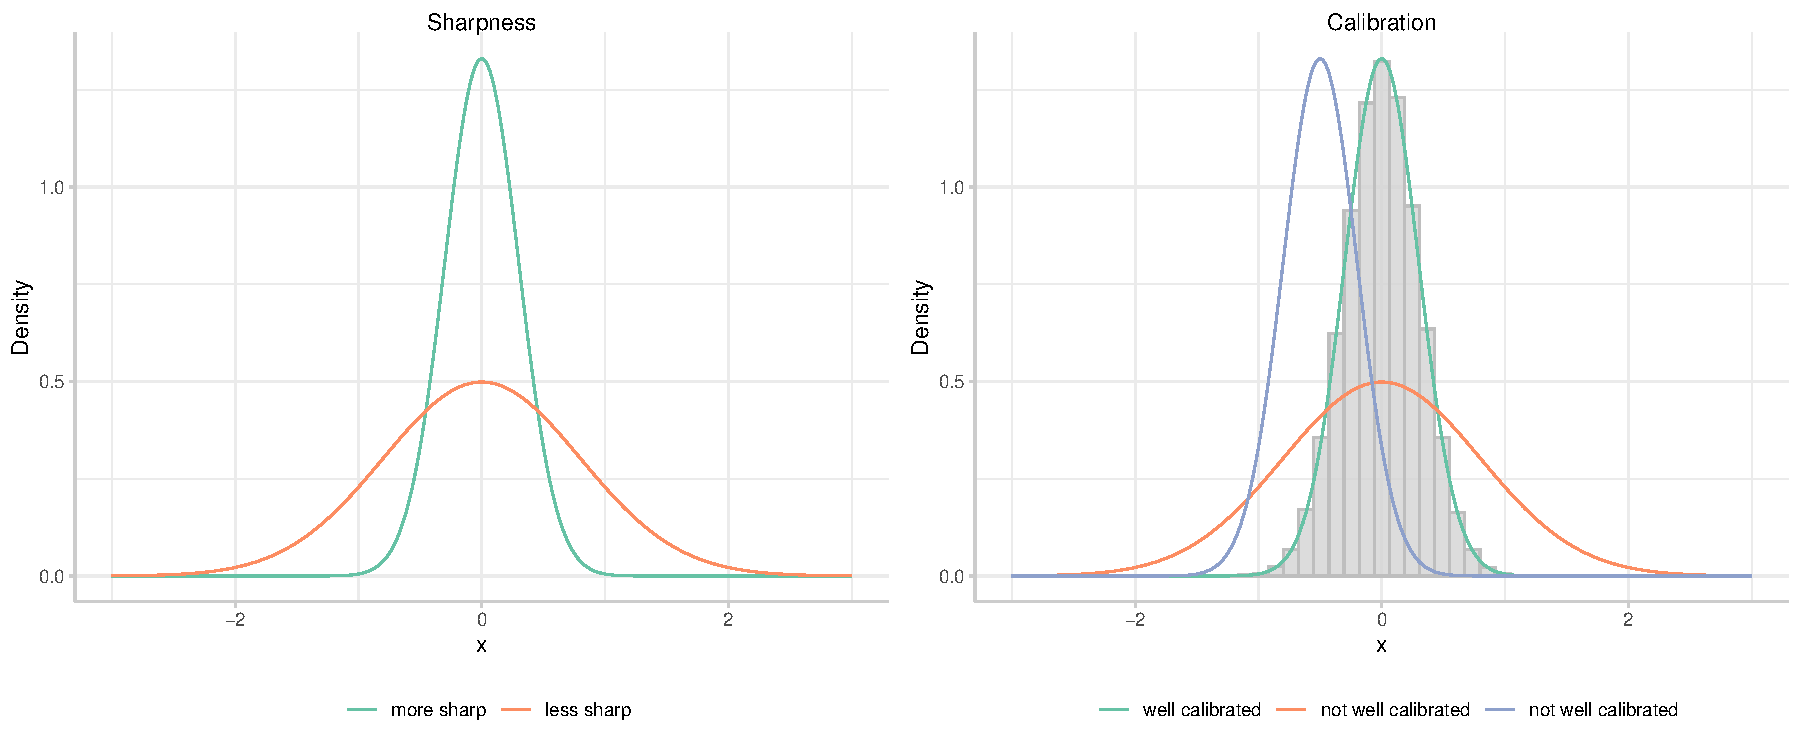
\includegraphics[width = \textwidth]{../plots/sharp_calib.pdf}
\caption{Illustration of the concepts \textit{calibration} and \textit{sharpness}, as described by \cite{gneiting_probabilistic_2007}. Calibration refers to the statistical consistency between the predictive distributions and the observed values of the series, while sharpness is a quality of the predictive distributions only. The general guidance is that forecasters should maximize sharpness of the predictive distributions subject to calibration.}
\label{fig:sharpcalib}
\end{figure}
To better understand what an optimal forecast looks like and, in the same vein, how to best assess forecast performance, we follow the established and ubiquitous paradigm characterized by \cite{gneiting_probabilistic_2007}: an optimal forecasts should maximize \textit{sharpness subject to calibration}. We will now briefly explain this concept.\\
Consider that we aim to make a probabilistic forecast $F_t$ for a quantity $y_t$ at time $t$, which follows the distribution $G_t$. The ideal forecaster would thus issue 
\begin{equation*}
	F_t = G_t
\end{equation*}
as their probabilistic forecast. In practice, $y_t$ will eventually be observed, while $G_t$ remains an unknown and hypothetical theoretical concept. The skill of the forecaster thus needs to be judged based on the forecast-observation pairs $(F_t, y_t)$ - \cite{gneiting_probabilistic_2007} suggest to base this assessment on the concepts calibration and sharpness, which are visualized in Figure \ref{fig:sharpcalib}. \\
In their words, calibration refers to the statistical consistency between the predictive distributions $(F_t)_{t = 1,2,..}$ and the observations $(y_t)_{t = 1,2,..}$ and is comprised of different modes - see \cite{gneiting_probabilistic_2007} for a full characterization of the concept.   %Perhaps the most relevant in practice, marginal calibration refers to the limits of the two distributions being equal. 
Sharpness is a feature of the predictive distribution only and simply refers to the concentration of the predictive distribution. In short, they establish the result that the notion of an ideal forecaster is equivalent to the forecaster maximizing sharpness subject to calibration. In turn, this means that calibration is not a sufficient, but a necessary condition of an optimal forecast. When assessing forecast performance, both characteristics thus need to be judged and accounted for.\\
We will first introduce methods to assess calibration and afterwards turn to proper scoring rules, which summarize the notion in a single number.(?????)
\subsection{Assessing calibration}
The form of calibration that focus usually lies on is probabilistic calibration \citep{bosse_evaluating_2022}. A forecast can be regarded as probabilistically calibrated if, for a given quantile level $\tau \in (0,1)$ , the proportion of observations falling below this quantile over time is also equal to $\tau$. A natural and straightforward way to thus assess probabilistic calibration is by assessing the rates by which the observations are in line with the predictive distribution's quantiles, both in terms of the quantiles themselves and the central prediction intervals they induce. We thereby analyze the predictive distribution's \textit{coverage}, described in more detail in the following.
\subsubsection{Coverage}
%Coverage assesses forecast calibration by measuring the proportion of observations that fall into the predictive distribution's respective ranges over time and comparing this to $nominal$ coverage, that is, the ideally expected coverage. Coverage is thus a suitable assessment of probabilistic calibration of forecasts. 
\begin{figure}
\centering
\includegraphics[width = \textwidth]{../plots/intro_cvrg.pdf}
\caption{Central interval (I) and quantile coverage (II) rates of two component forecasts in the European COVID-19 Forecast Hub. Coverage rates can be used to assess a forecast distribution's probabilistic calibration. }
\label{fig:intro_cvg}
\end{figure}
Interval coverage measures the proportion of observations that fall into a central prediction interval of the distribution. For instance, for the central $50\%$ prediction interval, all observations that fell within the predictive distribution's $25\%$ and $75\%$ quantiles at the respective points in time are counted and divided by the total number of observations - the goal is to be as close as possible to the nominal coverage rate of $50\%$. Generally, a predictive distribution that is too wide and thus covers too many observations is called under-confident or conservative, while one that is too narrow is conversely called over-confident \cite{bosse_evaluating_2022}. Panel (I) of Figure \ref{fig:intro_cvg} exemplary shows coverage rates for two models: model A's empirical interval coverage generally stays close to nominal coverage rates as indicated by the diagonal line, while model B's empirical interval coverage is generally too low, making the model generally over-confident. %By assessing this for several central prediction intervals, we can additionally assess marginal calibration, that is, the congruence of the limit\footnote{We are of course only approximating by our sad finite sample ways.} distribution of the predictions with the true limit distribution as exhibited by the observed data \cite{gneiting_probabilistic_2007}. 
Within the literature around forecasting COVID-19, it is common to assess empirical interval coverage at the $50\%$ and $90\%$ or $95\%$ levels, to assess both the central tendency as well as the tail behavior of the predictive distributions.\medskip\\% We generally decide to favor reporting $90\%$ intervals, as the number of observations we have is not super large. \medskip\\
Quantile coverage directly measures the proportion of observations that fall below a given quantile of the predictive distribution. It can thus convey more information than interval coverage, which does not distinguish between the upper and lower quantile of the central prediction interval. For instance, a predictive distribution could exhibit good performance at the lower tail end of the distribution, but not at the upper end, which quantile coverage can more directly diagnose. For instance, panel (II) of Figure \ref{fig:intro_cvg} shows that model B's lower quantiles are generally set too high and upper quantiles are more in line with the observed data, resulting in overall too narrow prediction intervals as well as upward bias. Model A also shows some light upward bias that is more uniformly spread across the prediction quantiles. \medskip \\
Lastly, coverage deviation summarizes the above by averaging over the observed deviations between the empirical and nominal coverage for a set of central prediction intervals, thus resulting in a parsimonious way to assess coverage across several intervals that are of interest. This however comes at the cost of losing some information, in particular, which of the intervals has better or worse coverage. Moreover, multiple coverage deviations with opposite signs might cancel out in the aggregate, thus portraying a forecast model more favorable than it is in actuality.\\   
%%%%%%%%%%%%Then, show coverage plot of three examplary models%%%%%%%%%%%%%%%%%%
Due to the nature of assessing rates by which observations fall into specific intervals, we generally need a sufficiently large sample to assess coverage. \\
%Also, we again want to note . A common counterexample is predicting daily temperatures . Over time, such a forecaster can expect to see perf.  Thus, a model can ``hide'' behind good coverage in the aggregate. Assessing calibration in general is thus more a necessary rather than a sufficient condition for good forecast performance. However, it is still a very useful diagnostic tool that can help forecasters assess whether they are generally over- or under-confident.\\ 
%Prediction interval coverage measures the proportion of values that fell into a predictive interval of a given level and thus reflects how well a model was able to characterize uncertainty over time.\citep{cramer_evaluation_2022} \todos{(from SI, cite something better. Scoringutils paper is also a good reference)}. It measures probabilistic calibration \citep{bosse_evaluating_2022}.
\subsubsection{Bias}
To assess whether a forecasting model is biased, that is, systematically over- or underpredicts the target of interest, one can utilize the bias metric as proposed by \cite{funk_assessing_nodate}. For integer-valued forecasts, they suggest the following metric:
\begin{equation*}
B(F_t, y_t) = 1 - (F_t(y_t) + F_t(y_t + 1)).
\end{equation*}
In terms of bias, the ideal forecast would have exactly half its probability mass above and below the true value $y_t$, respectively. If this is exactly the case, the metric assigns a value of zero - otherwise, if the probability mass is unequally distributed, the forecast receives a penalty. If more probability mass lies below  the true value than above it, bias is negative - the extreme case thus occurs when the entire probability mass lies below true value, where we get $B_t = -1$. The opposite applies in the case where more probability mass lies above the true value. Thus, bias measures a forecast's general tendency to relatively over- or underpredict the target.\\
\cite{bosse_evaluating_2022} extend the bias metric for quantile-based forecasts as follows. If the true value $y_t$ is below the predicted median forecast $q_{t,0.5}$, the bias is 
\begin{equation*}
B(F_t, y_t) = 1 - 2 \cdot \text{max}\{\tau | q_{t,\tau} \leq y_t \}.
\end{equation*}
Similarly, if the true value $y_t$ is above the median forecast $q_{t,0.5}$, it is
\begin{equation*}
B(F_t, y_t) = 1 - 2 \cdot \text{min}\{\tau | q_{t,\tau} \geq y_t \}.
\end{equation*}
This can be interpreted as twice the difference between the quantile level that would ideally be closest to the observed data $y_t$ ($\tau = 0.5$, since the median would be the ideal prediction) and the quantile level that is actually most in line with it. If the observed value directly coincides with the median prediction $q_{t, 0.5}$, bias is zero, otherwise, the forecast receives a penalty. Concretely, if we interpret the quantiles as the endpoints of (central) prediction intervals, this is the outermost quantile of the predictive distribution such that the interval still contains the observed value $y_t$. As above, if the entire predictive mass is above or below the observed value, bias should take on the values 1 and -1, respectively. This is achieved by simply setting $q_{t,0} = 0$ and $q_{t,1} = \infty$.\\
Thus, in short, the further the central mass of the predictive distribution is from the observed value, the larger the bias.\\
An important feature of the bias metric is that it is bound to the interval $[-1,1]$ and thereby scores forecasts on a relative rather than an absolute scale - this means that we can directly compare different targets, even if their value ranges differ substantially.
In the next subsection, we introduce the weighted interval score, which also includes penalties for over- and underprediction. However, as \citep{bosse_evaluating_2022} remark, it does so on an absolute scale - the potential issue with this is that there are no ``ideal'' absolute values for over- and underprediction and these values can thus not be directly translated into an assessment of systematic bias. To give an example, a forecast might overshoot a particular target during high incidence times, leading to a high absolute penalty in terms of overprediction, which will dominate its overall scores - this however might mask a potential tendency of that some forecast to normally underpredict, which would however be reflected in the bias metric.\\
``It largely depends on the application whether one is more interested in the tendency to be biased or in the absolute value of over- and underpredictions'' \citep{bosse_evaluating_2022}.
\subsection{Proper scoring rules}
Suppose that $y$ is the realization of a random variable under the true data-generating distribution $G$. The forecasting problem is defined by trying to issue a predictive probability distribution $F$ for the future realisation of this random variable. Further, denote $s(F,G)$ for the expectation of $\text{E}[s(F,y)]$. We then say that scoring rule $s$ is \textit{proper}, if 
\[s(G,G) \leq s(F,G).\]
Put into words, this means that the scoring rule is minimized if the true data-generating distribution is issued as the forecast distribution. Likewise, the scoring rule $s$ is \textit{strictly proper} for the strict inequality.
A (strictly) proper scoring rule thus incentivizes the forecaster to issue his or her true belief for the predictive probability distribution.\\
This notion of the propriety of scoring rules originated with \todos{Winkler and Murphy (1968)} and its importance in the forecasting world (hmpf) cannot be overstated - if a scoring rule for a probabilistic forecasts is not proper, it could, for instance, incentivize a forecaster to report a more confident estimate than they actually believe in.\\
Mention that aggregating across locations/... preserves propriety \citep{bracher_evaluating_2021}.\\
We also want to note here that the specific scoring rule used in an application is not a meaningless choice: as will be demonstrated in later sections, different scoring rules in practice usually induce different rankings of forecasts. In practice, the guidance is thus usually to consider several scoring rules - sometimes, a stakeholders' or decision makers might also exhibit a certain preference for forecast performance, which can guide the choice.\\
Recall the concept of sharpness subject to calibration: scoring rules assess this.
%\subsubsection{PIT}
%One way to assess a forecast's probabilistic calibration, that is, the congruence of the proportion of observations falling below a given threshold as observed and as they are predicted by the forecast (that is, the predictive distribution's quantiles), is through the probability integral transform (PIT) histogram \citep{dawid_present_1984}.  \\
%The PIT is simply defined as the predictive cumulative distribution function's value at the observed value, that is, $p_t = F_t(y_t)$. If the forecast has good probabilistic calibration, we can expect a histogram of these transformed values to be approximately uniform. A \\
%However, these can be seen as a necessary, rather than as a sufficient condition for the validity of a forecast model \cite{gneiting_probabilistic_2007}. For example, a weather forecaster that always predicts with a location's yearly stationary temperature distribution would, if also judged at yearly resolution, receive a uniformly shaped (assuming no structural shifts in the temperature's distribution\footnote{Do I hear you say climate change?}), but would be of no real use.
\subsubsection{Weighted Interval Score} \label{ssub:weighted_interval_score}
Here, we introduce the \ac{wis}, which is the main scoring rule used within this thesis \cite{bracher_evaluating_2021}. It is designed for use on probabilistic forecasts  $F$ that are issued as a set of discrete central prediction intervals, each with nominal coverage level $\alpha$ - or, put differently, as a set of symmetric predictive quantiles $q$ which directly translate to central prediction intervals. \\
Each central prediction interval can be scored via the interval score \citep{gneiting_strictly_2007}
\begin{equation}
IS_{\alpha}(F, y) = (u-l) + \frac{2}{\alpha}(l - y)\mathbb{1}(y < l) + \frac{2}{\alpha}(y - u)\mathbb{1}(y > u),
\end{equation}
where $\mathbb{1}$ is the indicator function, returning 1 if the condition inside the parentheses is fulfilled and 0 otherwise. The three summands each have an intuitive interpretation. The second and third summands express under- and over-prediction, respectively. They assign a penalty if the true observed quantity $y$ falls below (above) the lower (upper) endpoint $l$ ($u$) of the prediction interval. The first $(u-l)$ expresses the width of the central prediction interval and thus the sharpness of the predictive distribution $F$ - if this term didn't exist, it would make sense to simply issue very large prediction intervals that are highly likely to contain the true observation $y$. These penalties are furthermore scaled by the nominal coverage level: a smaller $\alpha$, which corresponds to a higher nominal coverage rate, induces a higher penalty if $y$ does fall outside one of the endpoints. \\
\cite{bracher_evaluating_2021} extend this score for use on a predictive distribution $F$ that consists of a set of such intervals, each with unique coverage level $\alpha$. The set of interval scores is gathered and aggregated into the weighted interval score 
\begin{equation}
WIS_{\alpha_{0:K}}(F,y) = \frac{1}{K + 1/2}\left(w_{0}|y-m| + \sum_{k=1}^{K}\left(w_k IS_{\alpha_{k}}(F, y)\right)\right),
\end{equation}
where usually the quantile weights are set to $w_k = \frac{\alpha_{k}}{2}$, and the median weight to $w_{0} = \frac{1}{2}$.\\
It can be shown that the \ac{wis} is an approximation of the \ac{crps}, a well-known scoring function that measures the distance between the predictive and true distribution 
\begin{equation}
CRPS(F, x) = \int_{-\infty}^{\infty} \left(F(y) - \mathbb{1}(y \geq x) \right)^2dy.
\end{equation}
In contrast to the \ac{crps}, the WIS gives slightly larger weight to intervals with large nominal coverage \citep{bracher_evaluating_2021}.
All in all, the \ac{wis} is a parsimonious way to score forecasts that come in the shape of a set of discrete intervals \citep{sherratt_predictive_2022}. Its decomposition allows to understand it directly as summarizing the trade-off between coverage and precision. \\
An important characteristic of the WIS is that it is not standardized and thus scales with the data. This can be easily seen in equation ?, as the absolute differences of the observed value and the predicted quantile directly enter into the score. Thus, scores will usually increase if the target to be predicted increases, as this is usually associated with larger absolute deviations from the target. This can make forecast comparisons challenging, which leads us to the next point.
\subsection{Comparisons of forecasts} \label{sub:pairwise_comps}
An issue that often arises when aiming to compare different forecasting models is a potentially non-overlapping base of targets the models issued predictions for. As most scoring rules are not normalized and scale with the data, %For instance, if models were compared via average WIS, 
one model might look better than another in terms of simple average scores if it only predicted in periods that saw low incidence or that were otherwise comparatively "easy" to forecast \cite{cramer_evaluation_2022}. This would thus disincentivize forecasters to predict in periods that they perceive to be more challenging - this is especially undesirable because these periods (e.g. exponential growth, high level of infections) are often of special interest to decision makers \todos{(cite something)}.\\
One can address this by computing a relative score that is based on pairwise comparisons of models, as developed in \cite{cramer_evaluation_2022}. For a pair of models denoted $l$ and $m$, first a measure of relative skill is computed
\[
\theta_{l,m} = \frac{\bar{s}_{l}}{\bar{s}_{m}},
\]
where $\bar{s}_{l}$ and $\bar{s}_{m}$ denote the average scores the models achieved on the targets both models predicted on. In principle, one can base these comparison on any scoring rule that gives either exclusively positive or exclusively negative values, but we follow the relevant literature and thus the WIS.\\
For each model $l$, one then computes the 
\[
\theta_{l\cdot} = \left(\prod_{m = 1}^{M}\theta_{l,m} \right)^{\frac{1}{M}},
\]to obtain a relative score of model $l$ with respect to all other available models. The choice of the geometric mean as an aggregation function over models is convention in the literature, but \cite{ray_comparing_2022} show in their application that the choice of aggregation function is indeed not critical, and that one could thus also use an arithmetic mean. \\
This relative score can be interpreted as a performance measure of model $l$ with respect to a model with ``average'' performance. If interest lies in a direct pairwise comparison with a specific model $m$, one can instead consider the ratio of these relative scores
\begin{equation} \label{eq:mean_score_ratio}
\phi_{l,m} = \frac{\theta_{l\cdot}}{\theta_{m\cdot}}. 
\end{equation}
Calculating this ratio for all model pairs that are of interest results in a ``pairwise tournament'' for all models in the set - this approach is implemented in the \texttt{scoringutils} package \citep{bosse_epiforecastsscoringutils_2022}. For negatively oriented scoring rules, the ratio will be smaller than 1 if model $l$ outperformed model $m$ on their set of shared targets and larger than 1 if it did not. Note that this mode of pairwise comparison still requires the assumption that it is equally hard to perform relatively well to other models at all forecast dates and locations \citep{cramer_evaluation_2022}.\\
If one is interested in concisely summarizing the skill of single models rather than performing comparisons between all pairs of models, one can choose a baseline model's $B$ relative score $\theta_{B\cdot}$ as the denominator. When using the WIS as the scoring rule, this results in the measure that is commonly referred to as "relative WIS" \citep{cramer_evaluation_2022}. Analogously to above, a ratio below 1 corresponds to a model overall outperforming the baseline model, while a score above 1 means that the model did not succeed in clearing baseline performance.\\
In section \ref{sub:model_types_analysis}, we use these comparisons to compare groups of models, more specifically certain model types, against each other (better: compare relative skill?). As stated previously, averaging scores preserves propriety, making this comparison possible.\\
This method of comparing component forecasts was largely developed to address missingness in component forecasts and can thus be used to compare a larger number of models with differing amount of availability. When interest instead lies in directly comparing the performance of two specific models against each other, especially when one model is a more established ``benchmark model'' that the other model wants to win against, it can be more direct and natural to directly compare the average scores the two models obtained over all considered forecast dates and locations. This is also the approach taken by e.g. \cite{bosse_comparing_2021-1}.\\
%Lastly, we mention that missingness is only a problem that affects the component forecasters. In section XX ("Ensemble Experiments"), our ``alternative ensembles'' have perfect availability throughout the whole study period. We therefore feel it is more natural to directly scale the average aggregate scores the competing method obtained with those of the unweighted median that includes all component forecasters. As we are fundamentally interested in establishing an alternative to the already established benchmark rather than over individual component forecasts.\\
%``To enhance interpretability of scores we mainly report WIS relative to the Hub ensemble in the main text, i.e. we divided
%the average scores for a given model by the average score achieved by the Hub ensemble on the same set of
%forecasts (with values >1 implying worse and values <1 implying better performance than the Hub ensemble).''\cite{bosse_comparing_2021-1}.\\
Importantly, while this style of forecast comparison addresses the problem of non-overlapping models, it is still based on average scores and is thus most heavily influenced by targets with large nominal scores. Wherever possible, we thus 
\subsection{Model distance}
We so far discussed scoring rules, which, as stated, are used to assess the pairs $(F_t, y_t)$. In contrast to this, divergence functions $d$ are used to assess distance between a pair of distribution functions ($F_t$, $F'_t$) \citep{thorarinsdottir_using_2013}. This can be used to score the predictive distribution $F_t$ against an estimate of the true data generating distribution $\hat{G}_t$, but also to measure the distance between two competing predictive distributions $F_t$ and $H_t$. As it is fundamentally a measure of distance, the divergence function needs to fulfill $d(F,F)$ = 0 and $d(F,H)\geq 0$ for all $F$ and $H$. Furthermore, as they can be used to score a predictive distribution, it also needs to fulfill the notion of propriety as defined previously. Analogously to before, this means that. \\
The distance function we will use within the context of this thesis is the 2-order Cramer distance or integrated quadratic distance \cite{thorarinsdottir_using_2013}. It is defined as the integral
\begin{equation}
\text{CD}(F, H) = \int_{-\infty}^{\infty}\left(F(t) - H(t) \right)^2dt
\end{equation}
Incidentally, this is the divergence function associated with the CRPS as defined previously - this means that if a point forecast is issued instead, it reduces to the CRPS.\\
\cite{wang_covidhubutils_2022} developed an approximation of the Cramer distance for (potentially unequally-spaced) quantile-based forecasts as follows:
\begin{equation}
\text{CD}(F,H) \approx \sum_{i = 1}^{2K-1} (a_i^F - a_i^H)^2 (q_{i+1}^{P} - q_{i}^{P}),
\end{equation} 
where $q^P$ contains the $2K$ pooled and ordered predictive quantiles\footnote{With a slight abuse of notation as the subscript $i$ in this case indexes the position in the vector $q^P$, whereas usually the subscript refers to the quantile level $\tau$. However, since $\tau \in (0,1)$, and is thus strictly smaller than 1, and $i \in \{1,2,...,2K\}$, and is thus larger than 1, we believe the distinction is clear enough.} from $F$ and $H$ and $a_i^F$ is a vector that, for each quantile $q_i$ in the pooled quantile vector, contains the minimum quantile level $\tau$ for which the associated quantile $q_\tau^F$ is larger than it. We write this condition as
\begin{equation*}
a_i^F = \text{min}\{\tau | q_\tau^F \geq q_i^P\},
\end{equation*}
with an analogous definition for $H$. SImilarly to the scoring rules discussed above, the Cramer distance also scales with the data,
%Some characteristics: on the scale of the data $y_t$.\\
%Explain some characteristics of the Cramer distance, i.e. that it gives small distance to distributions that are wide. Investigate this a bit.\\
\subsection{Ensemble Techniques} \label{sub:ensemble_techniques}
There are several different techniques for consolidating a set of component forecasts into a single ensemble forecast, with research ongoing on what the best method is. Certainly, the most widespread methods for combining quantile-based forecasts are those that use a quantile-wise mean or median, with the additional option to more heavily place weights on certain component forecasts.\\ 
The (weighted) mean and median are also the methods that we use within this thesis, but note that other techniques are also possible. For instance, one could first derive a continuous probability distribution for each quantile-based forecast, and subsequently average these, before again taking discrete quantiles from the combined predictive distribution. To our knowledge, these techniques were experimentally tried for application in the U.S. Hub, without promising gains in performance. Additionally, it is possible to combine the mean and median approach with trimming methods, which - broadly speaking - remove a pre-determined number of most extreme valued forecasts before combining the remaining ones. An extensive evaluation of these methods was performed in \cite{taylor_combining_2021}, also without clear gains in performance.\\
For the mean ensemble, each quantile of the ensemble forecast is simply computed as the mean of that quantile from the component forecasts, that is
\begin{equation}
q^E_{t,h,\tau} = \sum_m^{M_t} w_{m,t} \cdot q_{m, t, h, \tau}.
\end{equation}
For an equally weighted mean ensemble, the weights are simply set to $w_{m,t} = \frac{1}{M_t}$ for all models, where $M_t$ is the number of models predicting for the given location and target series at time $t$.  \\
We define the weighted median as 
\begin{equation}
q^E_{t,h,\tau} = \text{min}\left\{q_{m^{*},t,h,\tau} \in Q^P_{t,h,\tau}: \sum_m^{M_t}  w_{m,t} \mathbb{1}\{q_{m,t,h,\tau} < q_{m^{*},t,h,\tau} \} = 0.5 \ \right\},
\end{equation}
where $Q^P_{t,h,\tau}$ denotes the pool of quantiles for level $\tau$ at time $t$ and horizon $h$ from all available component forecasters. The weighted median is thus the value for which the associated weight of all values smaller than it is half of the total weight, for which we have the common restriction $\sum_m^{M_t}w_m = 1$. If this value is not exactly attained within the pool of quantiles, linear interpolation is performed. For our purposes, we used the \texttt{weighted.median} function from the \texttt{spatstats} package \citep{baddeley_spatstat_2005}. Similarly to above, if we set $w_m = \frac{1}{M_t}$ for all models, we simply obtain the value which has half of all other values lying below it, that is, the regular median. \\
In Figure \ref{fig:ensemble_techs}, we show an example illustration of how the respective ensemble forecasts are formed for the case series in Germany, in this case from a set of 20 component forecasts. Especially at the upper end, predictive quantiles are fairly spread out - while most forecasters place the uppermost quantile ($\tau = 0.99$) to a value below $15000$, some issue substantially more wide predictive distributions, with the most extreme value just below $50000$. We can observe that the combination methods are differently impacted by these outlying forecasts, with ensembles based on the mean issuing larger forecasts for the upper quantile levels. The bigger resistance to outlying forecasts is a central feature of the median ensemble. \\
To determine weights for ensemble forecasts, several strategies have been proposed and applied in the literature, particularly around ensemble forecasts in the Hub papers. We mention those which we will also utilize within this thesis. \\
A straightforward way to weight forecasts is by setting weights inversely proportional to recent scores obtained by component forecasts, to our knowledge first applied in the literature around forecasting COVID-19 by \cite{bracher_pre-registered_2021}. The resulting weighting scheme is thus termed inverse score or inverse WIS weighting, with weights at time $t$ simply set to 
\begin{equation}
w_{m,t} = \frac{1}{\bar{s}_{m, t}},
\end{equation}
with
where $\bar{s}_{m, t}$ is the mean WIS value obtained by model $m$ over a rolling window of recently realized targets. It is thus computed as a simple moving average, that is
\begin{equation}
\bar{s}_{m,t} = \sum_{r = t-1}^{t-a}\sum_{h = 1}^{\text{min}\{r+h, t\}} \text{WIS}(q_{m, r, h, 1:K}, \ y_r).
\end{equation}
Note thus that targets that have not yet realized by the current forecast origin are excluded from the estimation. In a real-time setting, this is of course automatically enforced, while in a retroactive analysis such as here, combinations of forecast dates and horizons that lie in the future relative to the forecast origin need to be actively excluded.
\begin{figure}
\includegraphics[width = \textwidth]{../plots/ensemble_techns.pdf}
\caption{Demonstration of four ensembles resulting from a set of 20 component forecasts that issue forecasts for weekly incident cases in Germany on July 5, 2021 (Monday). The depicted forecasts are made for a two-week forecast horizon, with target date July 17, 2021 (Saturday). Note that forecast distributions are issued as a set of 23 non-equally spaced discrete quantiles (each one indicated by a tick on the y-axis), the depicted curves are thus interpolations between the quantiles. Component forecasts' predictive distributions are shown in grey, while the different ensemble forecasts are colored according to the legend. Ensemble forecasts are obtained by taking a (weighted) quantile-wise mean or median of component forecasts' quantiles - visually, for each quantile level on the y-axis, the component quantiles are horizontally combined. The weights for the weighted mean or median ensemble were obtained by inverse score weighting. Plot inspired by \cite{taylor_combining_2021}.}
\label{fig:ensemble_techs}
\end{figure}\\
Other scoring rules beside the WIS are in theory also possible, although we are not aware of any applications - the WIS remains the most natural choice, as it is the most parsimonious way to score forecasts in terms of both calibration and sharpness. The weights are subsequently normalized such that they sum to one. Regarding the possibility of models having missed forecasts within the window, different courses of actions are possible. These forecasts could be excluded from the weighting scheme entirely, which has the disadvantage of reducing the model set for the resulting ensemble. \cite{taylor_combining_2021} straightforwardly compute the average score based on only the available historical forecasts, but this can be problematic due to potentially favoring models that (perhaps even strategically) did not issue forecasts for targets that were perceived as difficult and consequently have a higher probability to induce larger scores. Alternatively, missing scores can be imputed, with \cite{bracher_national_2021} suggesting to impute a missing score by the worst score achieved by any model for that particular target. This can be regarded as a pragmatic approach to include all available models in the weighting scheme without disincentivizing participation in weeks that are perceived as difficult\footnote{maybe better: favor forecasts that shirked difficult weeks}, although it could potentially also skew weights in cases where outlying forecasts with large absolute scores exist within the relevant set of realized forecasts. Yet another possibility is to base estimation of weights on the relative WIS as described in section \ref{sub:pairwise_comps}, as is done in \cite{ray_comparing_2022}. This in effect also means that scores are imputed, although by an average score.\\
The window size $a$ is a parameter that effectively governs how much more distant historical forecasts impact the weight estimation. The more historical forecasts are considered, the smaller the variance of the weight estimation, while bias will reduce if we exclusively base weight estimation on more recently made forecasts (if we assume forecast performance to be non-stationary). Note also that the smaller the window size, the more weight is proportionally placed on forecasts that were made for shorter time horizons - for instance, if $a = 3$, only one three-week ahead and no four-week ahead forecast will have realized by the forecast origin. We would argue that this is somewhat desirable, as scores at longer horizons usually induce larger absolute scores and thus influence the weight estimation more. For larger windows, this effect somewhat disappears.\\
Due to the fact that performance of component models generally is non-stationary and more distant scores can thus be regarded as having less predictive power for current forecast performance, we additionally wanted to try an ex-ante weighting scheme applied to the scores themselves. This scheme should more heavily weights recent scores, while still including more distant scores, albeit to a lesser degree. A natural choice is thus an exponential smoothing approach, thus changing the computation to\\
\begin{equation}
\bar{s}_{m,t}^{e} = \sum_{r = t-1}^{t-a} \alpha \cdot (1-\alpha)^{(t-r-1)} \sum_{h = 1}^{\text{min}\{r+h, t\}} \text{WIS}(q_{m, r, h, \tau}, \ y_r).
\end{equation}
As we still use a rolling window and thus don't include all historical forecasts, we additionally scale the exponential smoothing weights such that they sum to one. While this nature of essentially cutting off observations after a certain lag is to our knowledge not usual practice for exponential smoothing approaches, we regard this as unproblematic. This is due to the fact that more distant forecast, due to the nature of the exponential decrease, would get very low weights anyway. Importantly, this practice however saves some trouble that arise with potentially missing forecasts. \\ 
Another possibility for weighting component forecasts that chooses weights such that they directly minimize the historical weighted interval score is implemented in the \texttt{quantgen} package \citep{tibshirani_quantgen_2020}. For this approach, weights are chosen according to the following objective function \\
\begin{equation} \label{eq:qra}
\underset{\bm{w}}{\text{min}} \sum_{k=1}^{K} \sum_{r = t-1}^{t-a} \psi_{\tau_k}(y_r - \sum_{m=1}^{M}w_m q_{r,m,k}),
\end{equation}
again with the restriction that the elements of the weight vector $\bm{w}$ must sum to one. $\psi_{\tau}$ is the ``pinball'' loss for quantile level $\tau \in (0,1)$, that is 
\begin{equation}
\psi_{\tau}(v) = \text{max}\{\tau v, (\tau-1)v\}.
\end{equation}
As can be seen in \cref{eq:qra}, the weight estimation method is based on minimizing scores by taking a weighted mean of the forecast distributions's quantiles. The natural choice is to consequently also use the resulting weights $w_m$ in a mean ensemble. \\
\cite{brooks_comparing_2020} found the resulting ensemble to be competitive to an equally weighted median ensemble, for forecasting COVID-19 deaths during the year 2020. An issue with this method as it is implemented is{} that it needs full data for all component forecasts within the relevant window. As weight estimation is based directly on the set of predictive quantiles, this makes imputation of missing values more challenging, contrary to the weighting methods based only on forecasts' scores. Furthermore, as the pinball loss scales with the target value, the method will generally is also generally vulnerable to be influenced by locations or single targets with larger absolute levels.\medskip\\
For all weighting methods, it is generally possible to allow for more flexibility and separately estimate weights for the different quantiles, as well as the forecast horizons. \cite{ray_comparing_2022} state that they did not observe any consistent improvements from such approaches, and accordingly resorted to simpler weighting schemes. In fact, additional issues could arise from such an approach. For instance, a desirable property of forecast distributions is that they have a widening cone of uncertainty with increasing forecast horizon, to account for the fact that uncertainty is generally greater for targets that lie farther in the future. This is generally also a feature that is upheld across single component forecasts - when different forecasts are however weighted unequally across horizons, this continuity could be disturbed. When allowing flexible weights across quantiles, one needs to incorporate noncrossing constraints. \\
For our study, we did however decide to generally estimate weights separately by location. We do this to counteract the effect of locations with higher observed values influencing the estimated weights too heavily, as well as to pragmatically account for the fact that the set of models varies considerably by location. Furthermore, weights are computed separately for the two target series (cases and deaths), which is common practice.\\
\newpage
\section{Data}
In this section, we introduce the data used in this thesis. We first generally introduce the European COVID-19 Forecast Hub, and then introduce the particular subset our work is based on.
\subsection{European COVID-19 Forecast Hub}
The data used in this thesis stem from the European COVID-19 Forecast Hub, thereafter referred to as the ``European Hub'' or just ``Hub'', which was instigated by the \ac{ecdc} in 2021 to collate forecasts for COVID-19 incidence cases and deaths from independent modeling teams, for 32 European countries \citep{sherratt_european_2022}.\footnote{Info for this section is taken from the Wiki at https://github.com/covid19-forecast-hub-europe} It was modeled after a similar previous effort in the United States, the United States COVID-19 Forecast Hub, thereafter referred to as the ``U.S. Hub'' \citep{cramer_united_2021}. Furthermore, the preceding German-Polish Forecast Hub was largely synchronized with the European Hub \citep{bracher_german_2020}. The Hub's primary goal is stated to "provide reliable information about the near-term epidemiology of the COVID-19 pandemic to the research and policy communities and the general public" \citep{sherratt_predictive_2022}.\\ 
In general, a modeling hub is a coordinated effort, in which one or more common prediction targets, as well as a common format for prediction, are agreed upon and centrally implemented \citep{reich_collaborative_2022}. This serves the purpose of facilitating model evaluation and development by making model predictions comparable, as well as making predictions suitable for aggregation, that is, for generating ensemble predictions. A central advantage of the ``Hub''-methodology is thus the potential to synthesize results from different modeling approaches and teams. Common concerns can thus be addressed - for instance, \cite{metcalf_opportunities_2017} remark that, following major disease outbreaks, there is often an explosion of modeling studies, but the usefulness of the thereby generated research is limited as quality of data and methods used vary, and there is often no follow-up for synthetication of results. %, somewhat passing up the opportunity to bring the field forward. 
The Hub format, in contrast to this, standardizes data quality\footnote{To a certain degree: In case of the European Hub, teams are free to use whatever data sources they wish, but are told that forecasts will be evaluated against the publicly available JHU data and are thus recommended to base their methods on the same data source. Furthermore, additional data sources for e.g. vaccination and testing data are recommended.} and facilitates evaluation and thus synthetication of results through a set of shared targets. The format has some precedence both in other fields, for instance climatology or ecology \citep{warszawski_inter-sectoral_2014}, as well as in epidemiology itself - some notable examples include forecasting influenza in the United States \citep{reich_collaborative_2019} as well as dengue fever in Puerto Rico and Peru \citep{johansson_open_2019}. 
\begin{figure}
\includegraphics[width = \textwidth]{plot_placeholder/visualize_data.png}
\caption{\todos{Replace with real plot.} Plot showing an example trajectory from the Czech Republic. Following the last available truth data point (on \todos{date}, modeling teams submit forecasts for one to four weeks into the future, respectively as a predictive distribution via a set of discrete quantiles. Pictured are the trajectories of the respective median predictions, with 90\% prediction intervals.}
\label{fig:czech_predictions}
\end{figure} \\
The common prediction targets for the COVID-19 Hubs are weekly incidence COVID-19 case and death counts in the respective locations (U.S. states, European countries). Later, hospitalization rates were also added as a target series to both Hubs, but we don't consider them within the scope of this work.\\ Forecasts are issued in a probabilistic manner, more specifically as a set of 23 quantiles of the predictive distribution, at non-equally-spaced levels between 0.01 and 0.99. Consider Figure \ref{fig:czech_predictions} for an illustration of the prediction format, in this case for case numbers in the Czech Republic, with the forecast date the \todos{date}. We can see that, ...\\ 
There were no restrictions for participation in the Hub, (meaning that in theory anyone could participate) and participating teams or individuals were free to only submit forecasts for any subset of combinations of locations and target types. Forecast dates were standardized and based on the \ac{ew} format as defined by the US \ac{cdc}, where each week starts on a Sunday and ends on the following Saturday. Forecasts were submitted by Monday and thus scored against the truth data as realized on the Saturday of the same week for 1-week ahead forecasts, and accordingly by the following Saturdays for larger forecast horizons.\\ 
The truth data source that models are evaluated against stem from \ac{jhu}, which collate and make available daily cumulative counts of cases and deaths. Since the Hub asks for weekly forecasts of incidence, the truth data is obtained by taking weekly differences of \ac{jhu} national data. This can in theory be problematic, as data are subject to revision and negative values for incidence counts are thus possible.\\
For both the European and the U.S. Hub, the central communication tool lies with the Hub ensemble, which was generally found to yield the most consistent performance for both target series, compared to the performance of single component forecasts. Both Hubs initially used a mean ensemble, but switched to the median ensemble after observing that it was more robust to occasional outlying forecasts. Subsequent evaluations also showed that the median outperformed the mean as a combination method for the ensemble (\cite{sherratt_european_2022}, \cite{ray_comparing_2022}). \\
To be included in the official Hub's ensemble, models had to provide a full set of 23 quantiles for all four forecast horizons, as well as pass a sequence of automated checks for their predictions, that is, that their quantile predictions were non-negative, integer-valued and did not cross \citep{sherratt_european_2022}.\\
The Hub also includes a baseline model, which is the same as the one that is used in the U.S. Hub. For each forecast origin, its forecast for the median incidence for both target series is equal to the value that was observed in the most recent week. For uncertainty around the median, the other predictive quantiles are taken from Monte Carlo approximations of the empirical distribution function that is induced by the first differences observed in the respective time series \citep{cramer_evaluation_2022}. In essence, this model can thus be seen as a random walk model with non-stationary variance.\\
Including a baseline model in a collective forecasting effort serves several goals: First, including such a ``naive'' model serves the purpose of providing a sort of ``minimum'' performance that models should be able to clear - a model having higher skill than the baseline thus gives validity to the performance of that model. Second, given the fact that most prominent scoring rules scale with the target and thus never obtain a sort of ``optimum'', reporting performance relative to the baseline is a pragmatic strategy to compare performance across dimensions.% which are usually not easily comparable.
Furthermore, adding a relative model that serves as a sort of measure of forecasting difficulty rather than relying on absolute performance also serves as a sort of dis-discouragement of inviting teams to forecast during periods that are perceived as more ``difficult'' than others (and which additionally also receive nominally very high scores). However, we want to note here that while the introduction of a baseline aims to fulfill the purpose of standardizing model comparison, it is not without alternative and its specific form can imp{}act model assessment \citep{sherratt_predictive_2022}. For instance, if the baseline model systematically performs worse during some periods, this might portray individual model performance more favorably - see section \ref{sub:model_types_analysis} for an example. We also refer to \cite{bracher_pre-registered_2021}, who, in their analysis of the German-Polish Hub, retroactively included alternative baseline to compare model performance against.\\
We also shortly discuss some differences between the European and U.S. Hub. The main difference pertains to the number of forecasters participating, as well as to participation continuity. Specifically, while the U.S. sees an average of between 30 and 40 submissions per week, most of which submit forecasts for all or most of the 50 U.S. states \citep{ray_comparing_2022}, the specific forecasters in the respective model sets as well as the total number of available models substantially varies by location in the European Hub. Furthermore, frequent entry and exit of forecasters (and thus less consistent records of past performance) are more of an issue in the European Hub. This comes with its challenges, which me mainly discuss in section \ref{sub:best_performers}. A less important difference between the two Hubs is the submission format: the U.S. Hub asks for a set of 23 quantiles for forecasting deaths and 7 quantiles for forecasting cases - in the European Hub, both submission formats are set to 23 quantiles.\\
Lastly, we discuss some differences in relation to forecasting the two target series, cases and deaths.\\
%\subsection{US forecast hub}
%Numerous studies have come out for the US forecast hub. Taylor and Taylor, Ray 2020. \cite{ray_ensemble_2020}. Write short summary on US and EU Hub forecast papers?\\
\subsection{Data subset} \label{sub:hub_data}
\begin{figure}
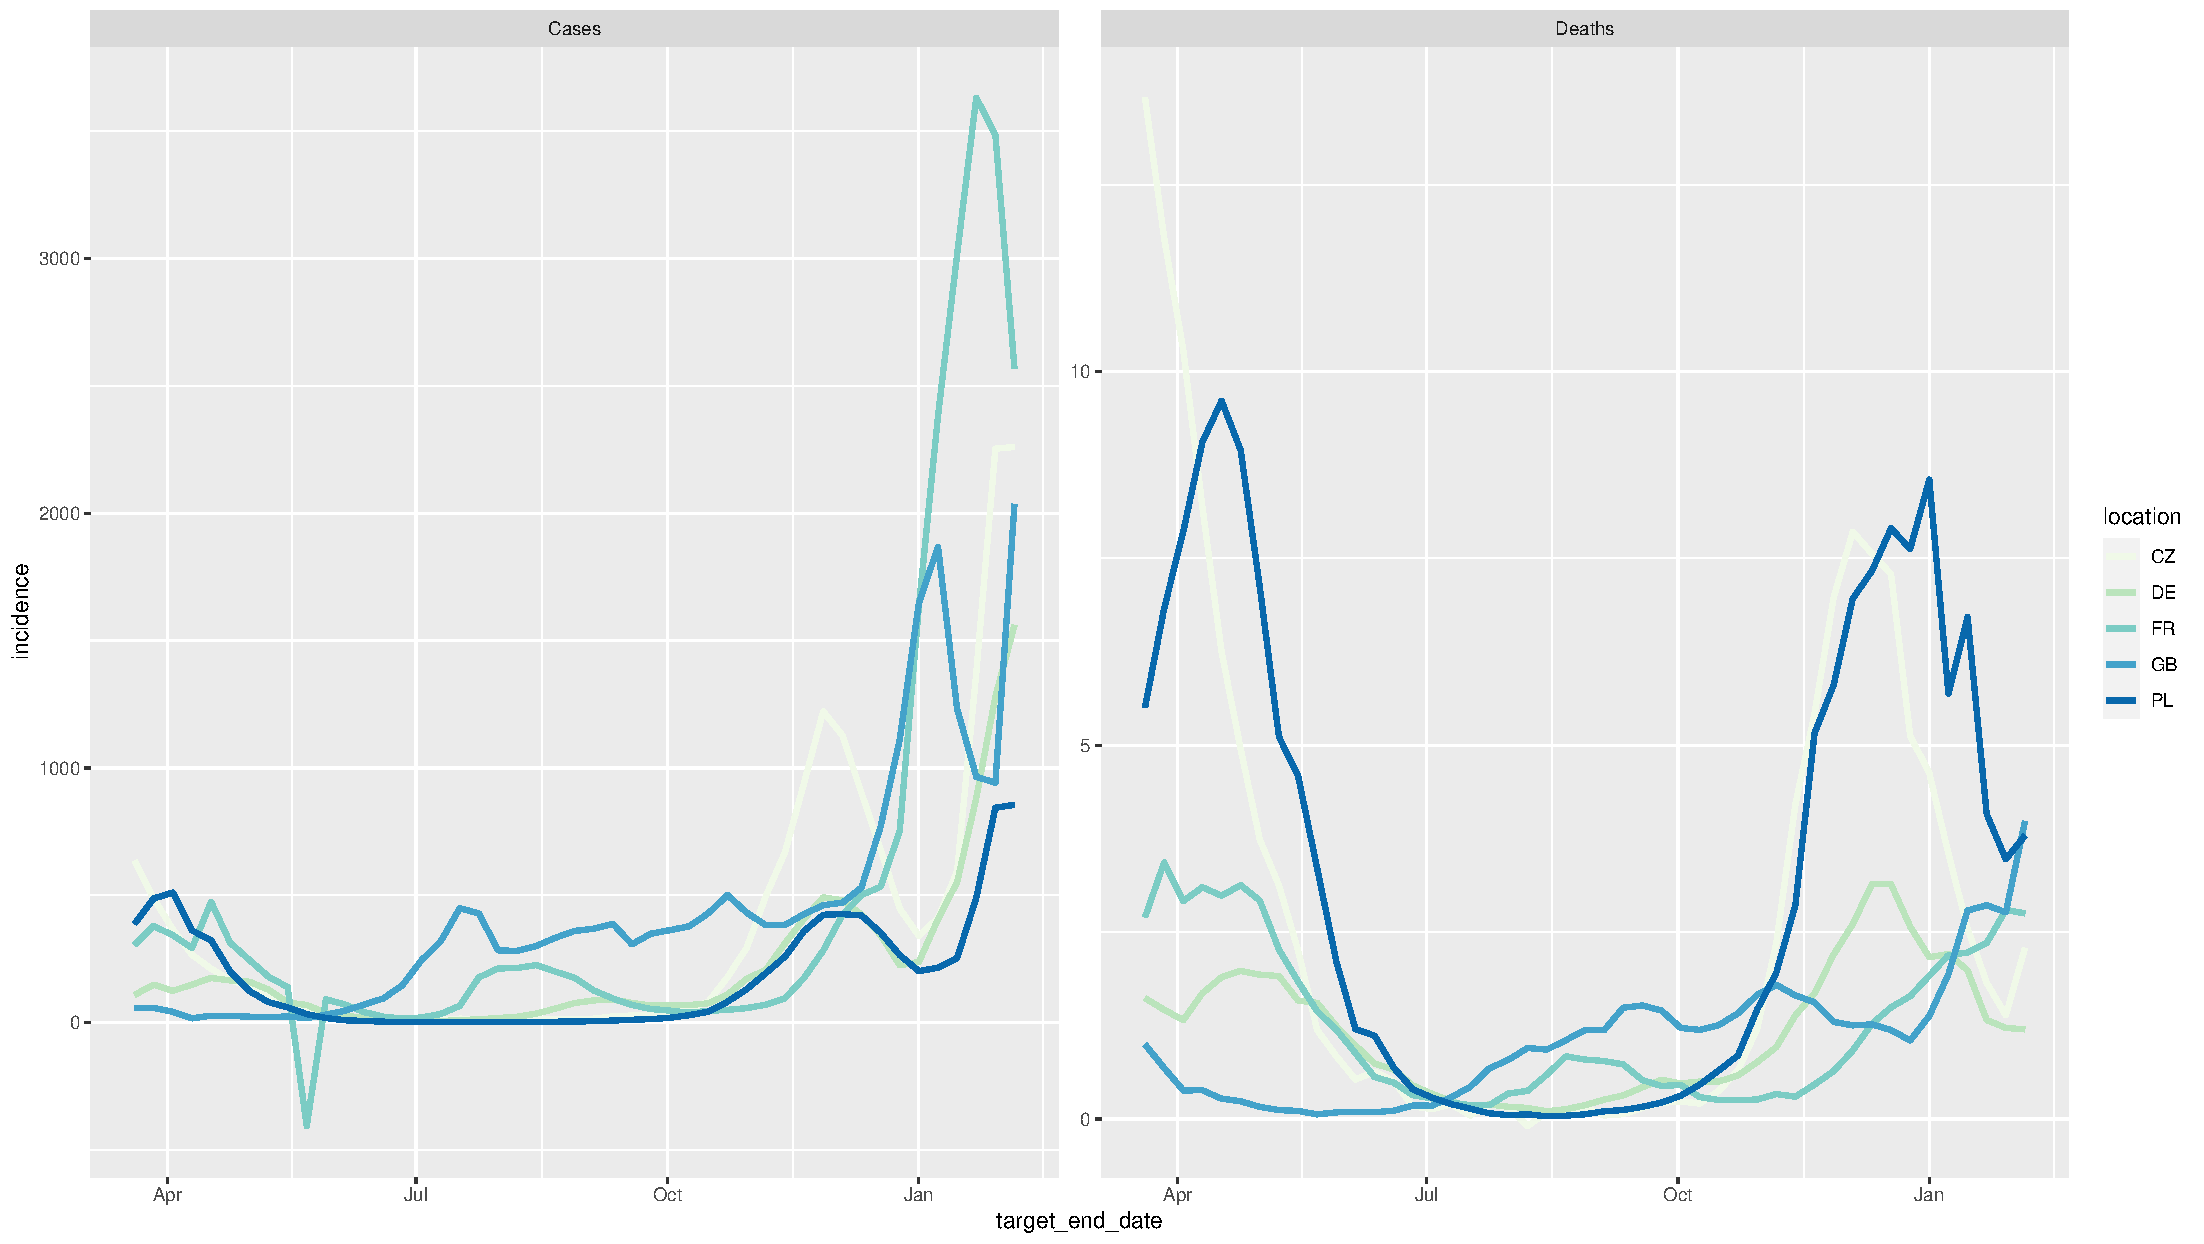
\includegraphics[width = \textwidth]{../plots/trajectories.pdf}
\caption{Trajectories of the cases and deaths series for the locations from the European COVID-19 Forecast Hub considered within this study. Note that the time series for cases were scaled by the respective location's population for readability. The time series for deaths are direct incidence counts.  A period categorization is highlighted . The equality of the y-axes is a coincidence.}
\label{fig:trajectories}
\end{figure}
\begin{figure}
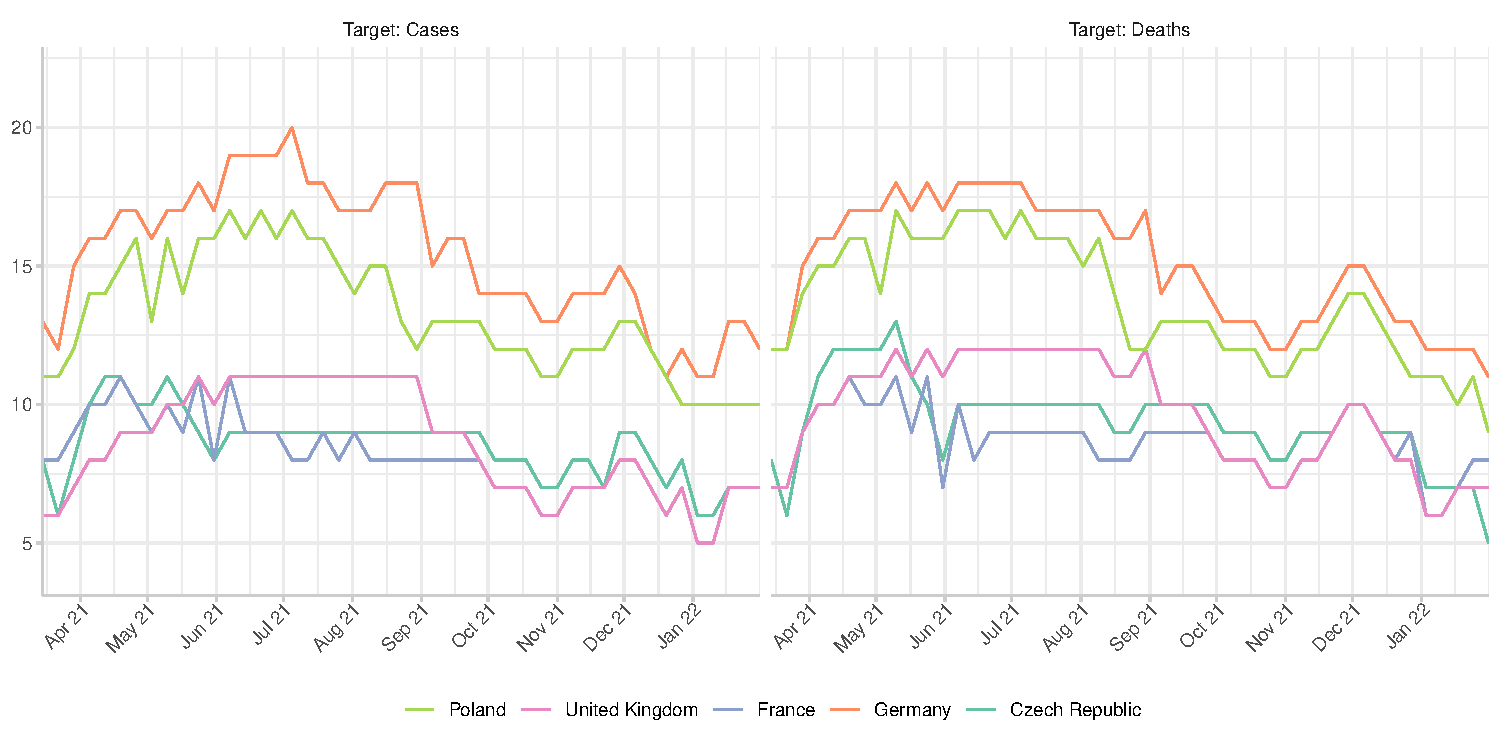
\includegraphics[width = \textwidth]{../plots/availability_overall.pdf}
\caption{Overall availability of component forecasts submitted to the European COVID-19 Forecast Hub for the five locations and two target series considered in this study, visualized over time and separately for the two target series (incidence cases and incidence deaths). Note that wherever the line plot for France or the Czech Republic isn't visible, it is overlain by that of the United Kingdom, as the locations have the same number of models during these times. As these plots show the availability of component forecasts, the European Hub baseline and ensemble model are excluded from the total number.}
\label{fig:avail_ovrl}
\end{figure}
\begin{figure}
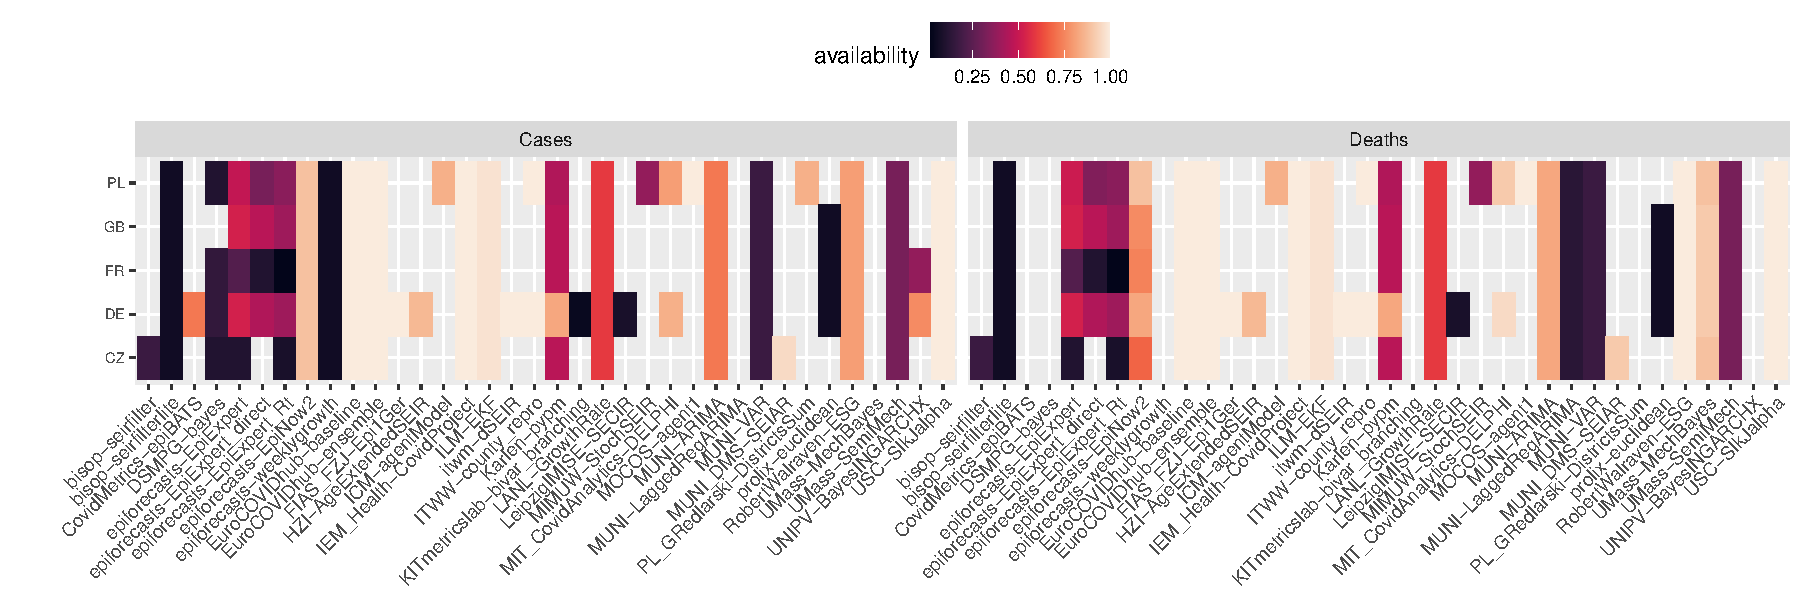
\includegraphics[width = \textwidth]{../plots/availability_indiv.pdf}
\caption{Availability of each model submitted to the European COVID-19 Forecast Hub for the five locations and two target series considered in this study. Availability was calculated as the proportion of the study period for which a model was available, for the given combination of location and target series. Missing panels refer to the case where a model never issued forecasts for a combination. Individual model availability generally varies, with only a small number of models participating for the entire period under study. Note that the European Hub baseline and official ensemble model are not shown, but do have perfect availability.}
\label{fig:avail_indiv}
\end{figure}
The subset of the European COVID-19 Forecast Hub that we base our analysis on comprises data from five European countries, with forecasts issued for both target series (cases and deahts) between March of 2021 and the end of January of 2022. \\
We restricted ourselves to the countries that had the largest base of models within the Hub - specifically, these are the Czech Republic, France, Germany, Poland and the United Kingdom. This is due to the fact that most of the analyses we aimed to perform required a sufficient model base as support. We decided to only use data up until the end of January of 2022 (and thereby targets that realized up until the end of February 2022), since heading into the spring months of 2022, various regulations and in particular testing criteria changed. We thought that this could make the time periods less comparable.\\
In Figure \ref{fig:trajectories}, we visualize the observed time series for the countries, separately for the two target series cases and deaths. We generally observe that while absolute values are often substantially different across countries and ``waves'' are not perfectly aligned, there nevertheless exist some common characteristics, such as generally lower incidence counts during the summer months as well as rising incidence towards the winter months, for both target series. As we will sometimes be interested in comparing forecast performance over time, but found that individual forecast dates provided too high of a resolution, we followed \cite{taylor_combining_2021} in dividing our study period into 10-week periods\footnote{since we have 47 weeks in our studied sample, we actually divide into 2 10-week and 3 9-week periods}. This categorization is also helpful, as scores are often dominated by higher levels of the underlying target series. These are indicated in the plot by the alternating grey background. While trends across locations naturally are not perfectly aligned, some common behavior can be observed: for cases, incidence numbers are declining at the beginning of the study period, followed by mostly (expect for the U.K.) lower levels in subsequent periods, which are however also characterized by intermittent rising levels. The series also show rising trends approaching the winter months, followed by the overall highest levels during the last period. For deaths, we similarly observe overall declining levels at the start of the study period and rising levels towards the end, although differences in absolute levels are not as high. The U.K., which also has higher case numbers during the summer months, also experiences higher mortality during the summer months.\\
We visualize total as well as individual model availability in Figures \ref{fig:avail_ovrl} and \ref{fig:avail_indiv}, respectively. Regarding the total number of available models by location, we observe that, after an initial period of uptake and recruiting, the modeling base is largest during the summer months and into the fall of 2021, after which it generally drops, with an intermittent slightly higher participation in December of 2021. Across countries, we observe that Poland and in particular Germany generally see higher participation, while the Czech Republic, France and the United Kingdom have a lower number of forecasters participating.\\
At the level of individual model availability, we also observe considerable fluctuations. Only a small number of models is available for the entire study period and across all locations, such as \texttt{IEM\_Health-CovidProject}, while others, such as \texttt{ITWW-country\_repro}, submit forecasts for the entire study period, but only for a subset of locations. Usually, we however see ``non-perfect'' availability for one or most locations, which can result from different base behavior: usually, this is due to modelers either starting participation at a later date and/or dropping out of the Hub entirely (such as e.g. \texttt{Karlen-pypm}), while others might only miss forecasting some weeks before subsequently participating again (such as e.g. \texttt{epiforecasts-EpiNow2}).
In general, this varying model base can be an issue. One can deal with these issues by e.g. only taking a full forecast set. However, we deliberately wanted to deal with the data as-is and develop and conceive strategies that work with and around this artefact of the data, as we felt that this was the most realistic and helpful for the situation at hand. \\
Recall our mention of the theoretically possible negative incidence counts in the previous section. In our subset of the data, this occured twice, once for the cases series in France and once for the deaths series in the Czech Republic - we excluded these observations and thus the forecasts that predicted for these particular targets.\\
We restricted ourselves to models that submitted the full set of 23 quantiles for each of the four horizons.\\
%For the US forecast hub, some things have worked well, most notably best performers or weighting. The question is whether we can also come to similar conclusions here. 
%Some differences to U.S. Hub: most notably, the model base. We thus always stratify by location, which they don't. Baseline model is the same. Furthermore, they require 7 predictive quantiles for cases, which however does not seem like a relevant difference.
\subsection{A short note on the nature of this study}
The analyses within this work will largely be devoid of rigorous statistical testing. Most of the works cited in this thesis that perform similarly perform retrospective forecast evaluations similarly are. There do exist methods to test the significance of differences in forecast scores/skill between models, the most common being the Diebold-Mariano test \citep{diebold_comparing_1995}, which however lacks an extension that accounts for correlations between forecasts issued for different target series and/or locations \citep{bracher_evaluating_2021}. \\
One could also conceive of a regression analysis with scores as the dependent variable, which could account for idiosyncrasies arising at certain locations or time points via e.g. the inclusion of random effects, but these also fundamentally suffer from the issue that scores are correlated across time and component forecasts, and that scores generally have large outliers which can heavily influence results and thus weaken the trust in reported p-values. Log-transforming the scores to bring them more in line with a normal distribution and reduce the effect is also not a viable alternative, as the log-transformation does not preserve the propriety of the scores, which is a vital feature, as it upholds the ordering of the models with respect to their closeness to the ``true'' distribution.\\ 
While we also find the resulting method of evaluation to a certain degree unsatisfactory, we feel that this approach is to a certain degree more honest than simply performing tests while being aware of these issues, the results of which could consequently not be trusted due to the aforementioned issues. We thereby follow the advice of \cite{bosse_evaluating_2022}, who due to these reasons generally advise against formal statistical testing ``in applied settings''.\\ 
We still think there is tremendous value in the analysis, but we are aware of and want to highlight the possible limitations. We argue that some of the knowledge distilled in this thesis should be checked against another year's results, to increase trust in the results. \\ 
We try to counteract this by carefully not masking trends in the aggregate, as well as also reporting results that did not show any striking conclusions.\footnote{aka all of our ``results''}. %Most of our analysis leads were furthermore defined from the start, and we refrained from \todos{(take this out, as it's not entirely true?)}.\\
%The nature of the European Hub data is such that...\\
%Furthermore, our methods are to a certain degree entirely descriptive. While for the ensemble experiments we try to imitate the real-time situation as much as possible, we are aware of the fact retrospective knowledge can creep in.\\
%%%%%%%%%%%%%%%%%%%%%%%%%%%%%%%%%%%%%%%%%%%%%%%%%%%%%%%%%%%%%%%%%%%%%%%%%%%%%%%%%%%%%%%%%%%%%%%%%%
%%%%%%%%%%%%%%%%%%%%%%%%%%%%%%%%%%%%%%%%%%%%%%%%%%%%%%%%%%%%%%%%%%%%%%%%%%%%%%%%%%%%%%%%%%%%%%%%%%
%%%%%%%%%%%%%%%%%%%%%%%%%%%%%%%%%%%%%%%%%%%%%%%%%%%%%%%%%%%%%%%%%%%%%%%%%%%%%%%%%%%%%%%%%%%%%%%%%%
%%%%%%%%%%%%%%%%%%%%%%%%%%%%%%%%%%%%%%%%%%%%%%%%%%%%%%%%%%%%%%%%%%%%%%%%%%%%%%%%%%%%%%%%%%%%%%%%%%
%%%%%%%%%%%%%%%%%%%%%%%%%%%%%%%%%%%%%%%%%%%%%%%%%%%%%%%%%%%%%%%%%%%%%%%%%%%%%%%%%%%%%%%%%%%%%%%%%%
%%%%%%%%%%%%%%%%%%%%%%%%%%%%%%%%%%%%%%%%%%%%%%%%%%%%%%%%%%%%%%%%%%%%%%%%%%%%%%%%%%%%%%%%%%%%%%%%%%
%%%%%%%%%%%%%%%%%%%%%%%%%%%%%%%%%%%%%%%%%%%%%%%%%%%%%%%%%%%%%%%%%%%%%%%%%%%%%%%%%%%%%%%%%%%%%%%%%%
%%%%%%%%%%%%%%%%%%%%%%%%%%%%%%%%%%%%%%%%%%%%%%%%%%%%%%%%%%%%%%%%%%%%%%%%%%%%%%%%%%%%%%%%%%%%%%%%%%
%%%%%%%%%%%%%%%%%%%%%%%%%%%%%%%%%%%%%%%%%%%%%%%%%%%%%%%%%%%%%%%%%%%%%%%%%%%%%%%%%%%%%%%%%%%%%%%%%%
\newpage
\section{Introspective Analyses}
In this section, we perform some more introspective analyses into model and ensemble performance within the European Forecast Hub. In the section following afterward, we consequently aim to explore whether some of the knowledge gained can be leveraged to establish methods that could in principle improve ensemble performance in real-time.\\
Specifically, we want to explore the performance of different modeling strategies, over the study period and the locations we consider in this study. Furthermore, we investigate the effect of adding a model to an existing ensemble, to better understand ensemble performance.
%%%%%%%%%%%%%%%%%%%%%%%%%%%%%%%%%%%%%%%%%%%%%%%%%%%%%%%%%%%%%%%%%%%%%%%%%%%%%
%%%%%%%%%%%%%%%%%%%%%%%%%%%%%%%%%%%%%%%%%%%%%%%%%%%%%%%%%%%%%%%%%%%%%%%%%%%%%
\subsection{Modeling Strategies} \label{sub:model_types_analysis}
%First and foremost, we had to categorize the models in the data in a meaningful manner. We decided on a categorization. To this end, we . Teams that mentioned an explicit compartmental structure of SIR or related (for instance SEIR, SECIR) type we categorized as "mechanistic".\\
As stated before, it remains an open inquiry of research which modeling strategy is best suited for epidemiological forecasting, specifically, whether it is necessary to explicitly include mechanistic assumptions to yield accurate predictions \citep{funk_short-term_nodate}.\\ %While for other diseases (such as influenza), statistical models have generally performed better.\\
In the case of forecasting COVID-19, \citep{bracher_evaluating_2021} state that they did not find any ``striking patterns'' between model strategies in their analysis, but also acknowledge that this might be due to the relatively short study period they considered (12 weeks). We thus want to investigate whether patterns can be found, given a longer study period..\\
We thus investigate performance at the level of the different modeling strategies as defined in section \ref{sub:ep_forecasting}. Since we are fundamentally interested in the question of improving ensemble performance
\begin{figure}
\centering{}
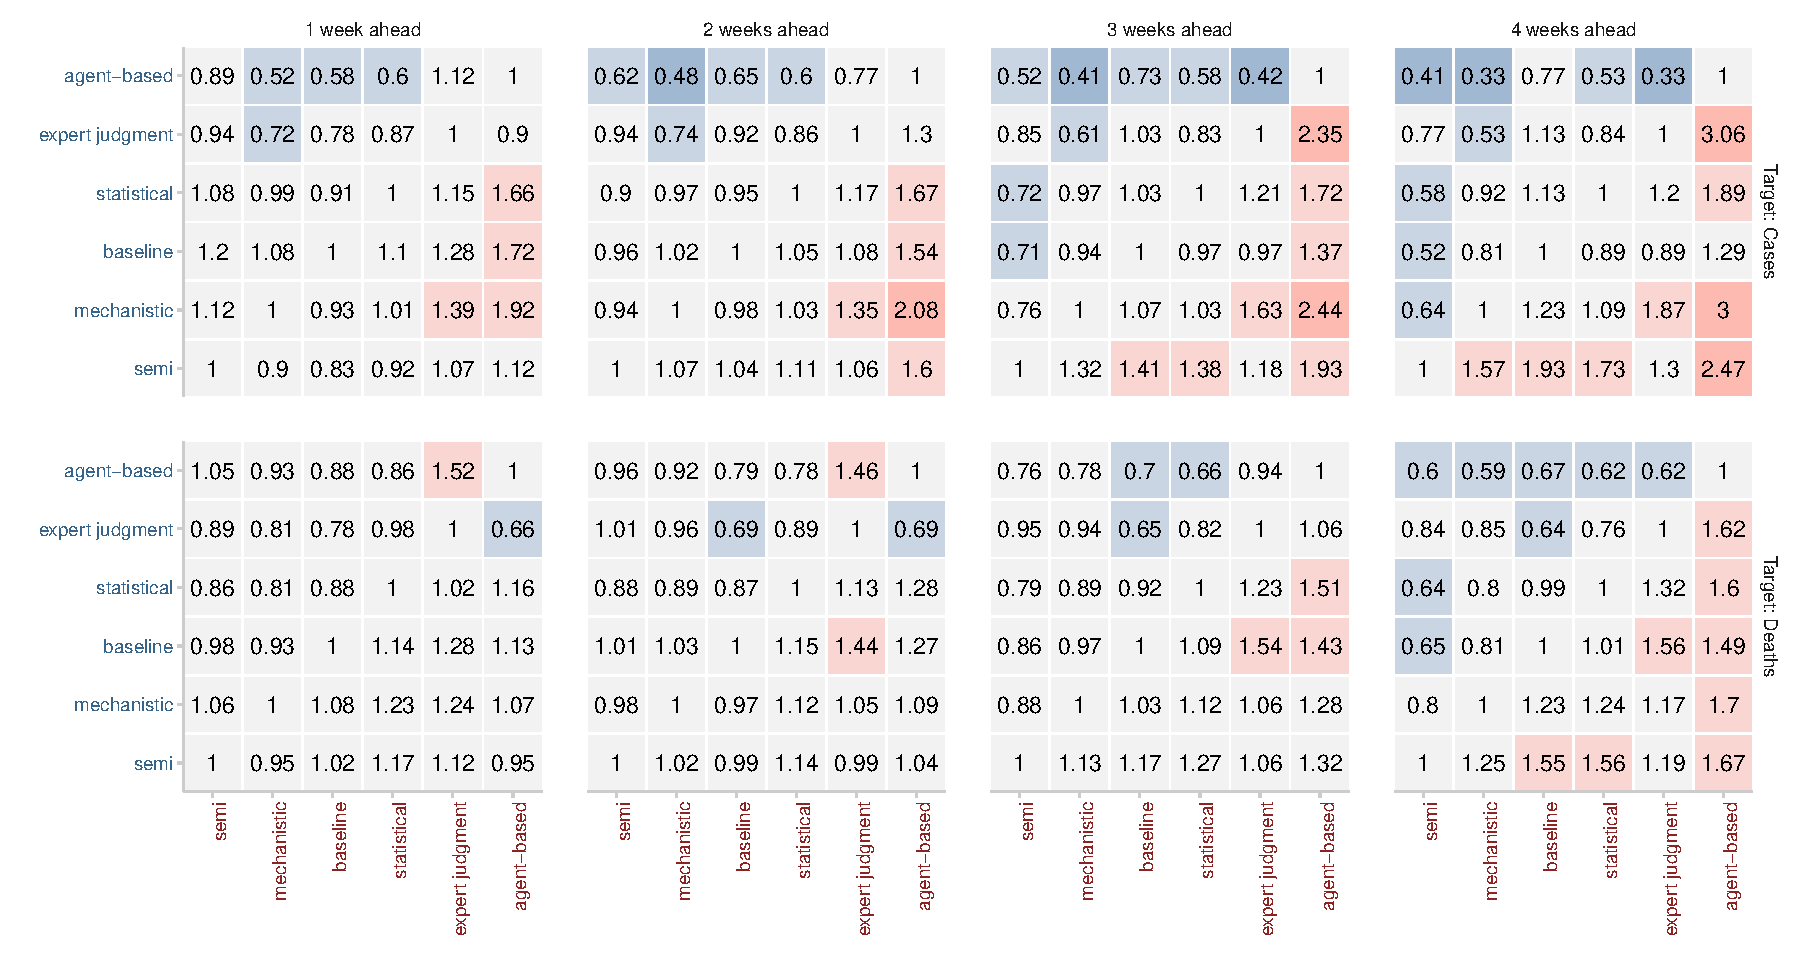
\includegraphics[width = \textwidth]{../plots/pw_comp_model_type_with_other_wide.pdf}
\caption{Pairwise comparison of model types. Plot was produced with package \texttt{scoringutils}}
\label{fig:pw_comp_modeltypes}
\end{figure}
%%%%%%%%%%%%%%%%%%%%%%%%%%%%%%%%%%%%%%%%%General intro to evaluation method/data base%%%%%%%%%%%%%%%%%%%%%%%%%%%%%%%%%%%
To investigate this question, we want to employ the methodology of pairwise comparisons as introduced in section \ref{sub:pairwise_comps} and apply them at the level of modeling strategies. Typically, the recommendation is to only compare models which are available for at least $50\% $ of the time period under study, to avoid comparison of forecasts that don't have any overlap \citep{bosse_epiforecastsscoringutils_2022}. Since we are comparing forecasts at the level of model types rather than single models and there does not exist a pair of model types without overlap in the relevant time period, this advice does not necessarily apply here. One could still make the argument that one should not exclude models that only contribute for a very small portion of the study period, so as not to have models that are perhaps more likely produce outlying forecasts\footnote{One could think that models that only have e.g. $10\%$ availability either dropped out due to not performing well and/or teams might have not been invested enough in the project to update and keep tuning their model, both of which might give low-quality predictions that as a result might not necessarily be representative of the respective model type.} influence the results too much - however, we found that the results were not at all sensitive to the exact choice of availability threshold chosen for the models, so we decided not to exclude any models here.\footnote{results from exclusions can be found in appendix} \\ 
Nevertheless, there remains the issue of the more obscure model types: as previously stated, the two agent-based models in the set only submitted forecasts for Poland, while the expert-judgment based models dropped out of the Hub during the late summer period of 2021. We report their results the highest level of aggregation (averaged results across all locations and forecast dates), but will mostly leave them out in the subsequent analyses, for conciseness and as we think that their performance is not as representative of a general modeling strategy. For a discussion of the relative performance of forecasts based on human judgment, we refer to \cite{bosse_comparing_2021}.\\ %Note that the value of the mean score ratio between two model types in the pairwise comparisons is independent of other models in the set, so the mean score ratios of the other pairs are unaffected by this choice \todos{WRONGGGGGG}.\\
%%%%%%%%%%%%%%%%%%%%%%%%%%%%%%%%%%%%%%%%%%%%Discuss pairwise comparisons%%%%%%%%%%%%%%%%%%%%%%%%%%%%%%%%%%%%%%%
The results of the pairwise comparison, where for each model type, weighted interval scores are stratified by horizon and target type, but averaged across the entire study period and all locations, can be found in Figure \ref{fig:pw_comp_modeltypes}. These plots show that the only modeling strategy that tends to show increased performance improvement over all other model types are agent-based models. It seems that, compared to other model types, they perform particularly well for forecasting case numbers, even more so at longer horizons. As previously mentioned, within our data set, these models only issue forecasts for Poland (for both the cases and deaths series), so the comparisons are purely based on data from that location. Thus, it is unclear whether their superior performance would transfer to other locations or settings. In particular, the other model types generally contain several models that issue forecasts for multiple locations, and one could argue that designing and tuning a model for a specific location lacks some of the potential complications that arise when aiming to establish a model with more universal application. We thus argue that comparability is somewhat limited.
\begin{figure}
\centering
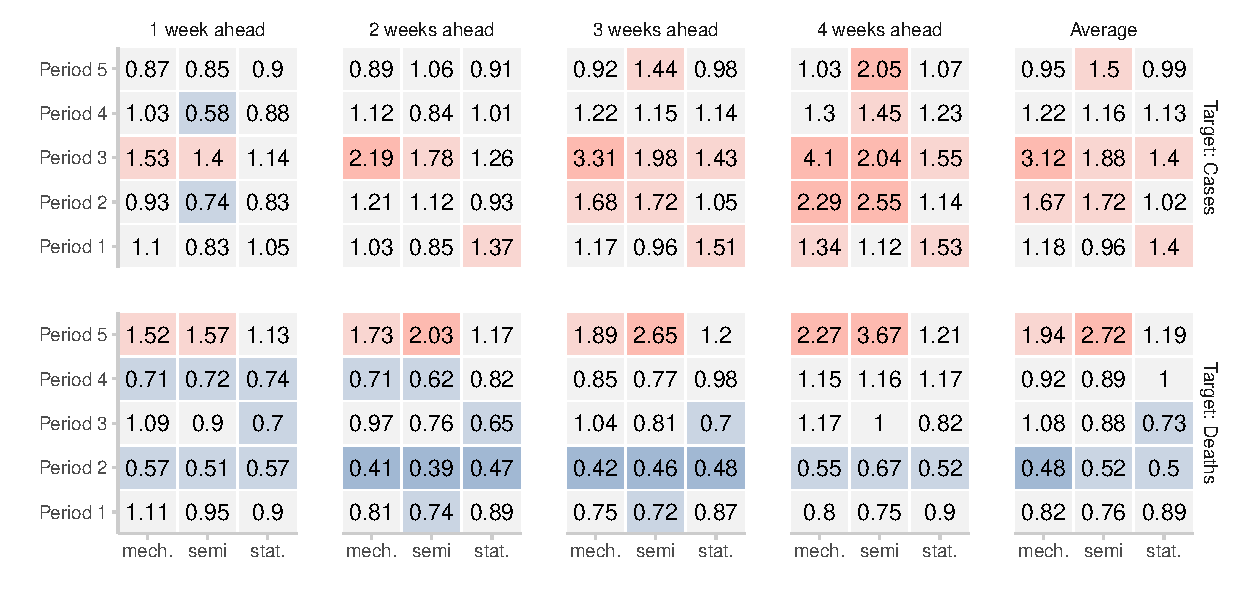
\includegraphics[width = 0.9\textwidth]{../plots/pw_comp_model_types_across_periods_wide.pdf}
\caption{Relative WIS resulting from pairwise comparisons of the dominant modeling strategies (mechanistic, semi-mechanistic, statistical) against the baseline model in the European Forecast Hub, for forecasting incidence cases and deaths during the time period March 2021 - January 2022. The time period under study is divided into two 10-week and three 9-week periods and comparisons are split up by the forecast horizon.  Results are averaged across the five locations considered in this study. Values above one mean that the respective modeling strategy on average performed worse than the baseline model for the given period, forecast horizon and target series. Correspondingly, values below one mean that it performed better than the baseline model. Lower relative scores of one model strategy compared to another similarly correspond to better performance. The code to produce this plot was adapted from the package \texttt{scoringutils} \citep{bosse_evaluating_2022}.}
\label{fig:pw_comp_modeltypes_byperiod}
\end{figure}
%Apart from this, we see some substantial differences in skill between expert judgment forecasts and mechanistic models for case forecasts. Upon investigation, \todos{(investigate where this comes from)} \\
Apart from this, mean score ratios mostly stay close to one, with some slight variations. In particular, statistical models, as well as the approaches based on expert judgment, perform similarly to or even slightly better than semi-mechanistic or mechanistic models. At least in the aggregate, we thus cannot confirm that explicitly modeling the epidemiological process gives an advantage in predictive performance. % This suggests that for issuing short-term forecasts for COVID-19, it might not be strictly necessary to explicitly account for and model epidemiological processes or transmission dynamics in order to achieve comparable/competitive forecast performance. 
In fact, at horizons three and four weeks ahead, semi-mechanistic models are outperformed by both mechanistic and statistical models for longer horizons, more so for forecasting cases than for forecasting deaths.\\ 
However, as previously stated, aggregate scores are generally vulnerable to be dominated by a small number of single targets that resulted in higher scores. It could thus be that this result only emerges from certain locations or time periods with higher incidence levels. Conversely, it could then be the case that while there are no consistent trends in the aggregate for either of the two series, there might be systematic differences in scores at lower resolutions. Put differently, it is perhaps overeager to assume that one model type could systematically outperform another over the entire study period, which, after all, comprises different countries with varying periods of infection dynamics, while patterns might exist at lower resolutions, that is, if comparisons are broken up by location or period. We investigate whether this is the case in the following. 
  %are , so they don't necessarily receive the same level of care and effort. As previosuly sta \\
%Of course, averaging across the entire study period and all locations has the issue of potentially masking some trends or effects, or worse, presenting trends in the aggregate that perhaps only spuriously result from diverging results at a lower resolution. Furthermore, as previously stated, average WIS scores are generally vulnerable to domination by periods and locations with high nominal incidence levels, thus making it possible that these results only stem from e.g. locations with larger populations. We thus want to consider results at lower resolutions (by horizon, individual locations and time periods).\\ %AS SCORES ARE HEAVILY INFLUENCED BY LARGER ABSOLUTE SCORES AND THUS DOMINATED BY LOCATIONS WITH HIGHER SCORES; AS WELL AS PERIODS WITH HIGHER SCORES AND LARGER HORIZONS; WE ALSO CONSIDER STRATIFICATION:\\ 
%First of all, we thus want to evaluate whether the results presented above describe a consistent trend across the entire time period, or whether these only stem from certain phases of the trajectories. We thereby follow \cite{taylor_combining_2021} in dividing our study period into 10-week periods\footnote{since we have 47 weeks in our studied sample, we actually divide into 2 10-week and 3 9-week periods}, to investigate differences emerge at lower resolutions. 
We thus perform the same pairwise comparisons, once stratified by period and horizon in Figure \ref{fig:pw_comp_modeltypes_byperiod}, and once stratified by period and location in Figure \ref{fig:pw_comp_modeltypes_byloc}. For conciseness, we refrain from showing all pairwise comparisons and only report performance against the baseline - as can easily be seen from equation \ref{eq:mean_score_ratio}, if a model type has a lower mean score ratio with respect to the baseline model than another model type, it will also outperform that model type in terms of their direct mean score ratio.
\begin{figure}
\centering
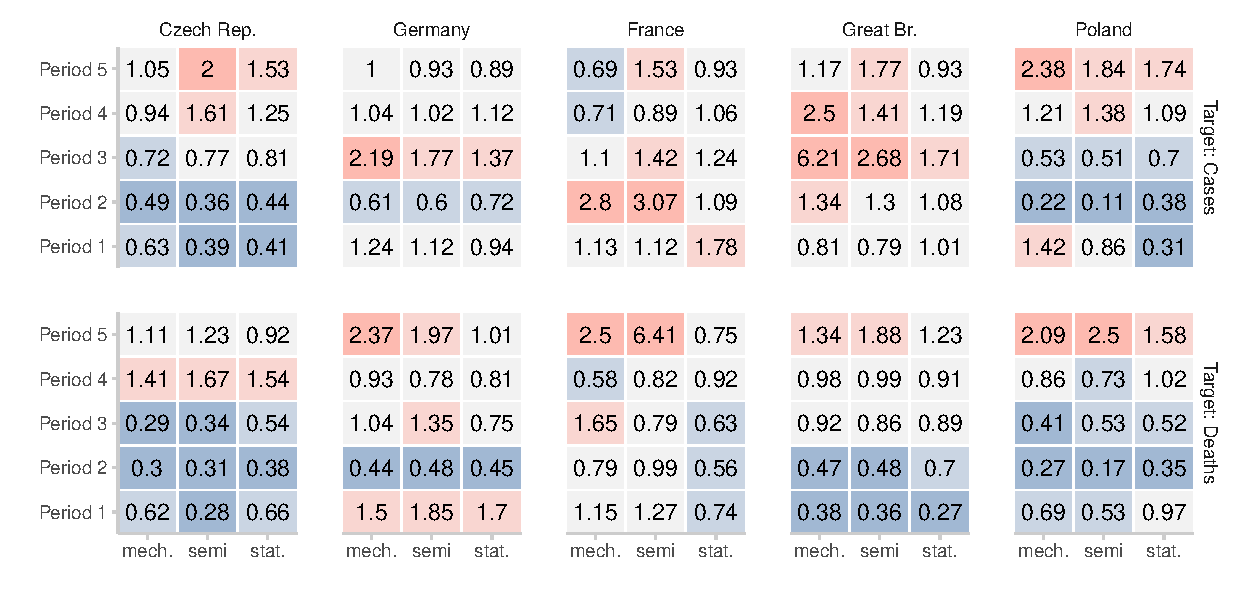
\includegraphics[width = 0.9\textwidth]{../plots/pw_comp_model_types_across_periods_and_loc_wide.pdf}
\caption{Relative WIS resulting from pairwise comparisons of the dominant modeling strategies (mechanistic, semi-mechanistic, statistical) against the baseline model in the European Forecast Hub, for forecasting incidence cases and deaths during the time period March 2021 - January 2022. The time period under study is divided into two 10-week and three 9-week periods and comparisons are split up by the locations considered in this study. Results are averaged across forecast horizons. Values above one mean that the respective modeling strategy on average performed worse than the baseline model for the given period, location and target series. Correspondingly, values below one mean that it performed better than the baseline model.  The code to produce this plot was adapted from the package \texttt{scoringutils} \citep{bosse_evaluating_2022}.}
\label{fig:pw_comp_modeltypes_byloc}
\end{figure}\medskip\\
First, consider Figure \ref{fig:pw_comp_modeltypes_byperiod}, which shows mean score ratios by period (and averaged across locations). While in the aggregate we observed that the different model types did not substantially outperform the baseline, breaking comparisons up by period reveals that the mean score ratio with respect to the baseline varies a bit more, showing both examples of under- and overperformance with respect to the baseline model. In fact, there is actually more variation in mean score rations between the different periods than between model types in a given period. That is, %it emerges that generally, 
the model types often collectively outperform the baseline model (e.g. for forecasting deaths in period 2) or collectively underperform/stay close in performance to the baseline model. Put more concretely, it appears that some periods are generally easier/harder to forecast in comparison to the baseline, and that performance differences between the model types are still not that pronounced. The same applies for many periods for the pairwise comparisons by location in Figure \ref{fig:pw_comp_modeltypes_byloc}. While examples of relative performance deterioration are evident for all groups, these seem to be less pronounced for statistical models - the worst mean score ratio received be the group of statistical models is 1.78, while the other two modeling strategies receive substantially higher values at times.\\
There are however some exceptions: notably, in most periods we observe that as forecast horizon increases for the cases series, relative performance of the semi-mechanistic models deteriorates. While this is to a certain degree also true of the other model types (especially in period 3), semi-mechanistic models critically receive high relative scores in period 5. As this is the period where incidence of cases is highest for all locations, this is likely the root cause of these models comparing unfavorably for longer horizons in the previously discussed aggregate.\\
Generally, the rankings that are induced by the mean score ratios for the model types mostly don't diverge between horizons. However, especially for forecasting cases, differences tend to get more pronounced, suggesting that differences in performance get exacerbated with rising forecast horizon.\\
At the level of individual locations, we again observe that semi-mechanistic models perform worse than other model types in period 5 for forecasting both cases and deaths, although differences are more or less pronounced for the different locations and series - for instance, performance is very similar in Germany for forecasting cases, whereas these models receive an especially high relative score in France for forecasting deaths. Apart from this, we do sometimes see differences in relative skill between the model types, although these often change by period and no striking pattern seems to emerge - although we did attempt to, it is difficult to determine the cause of these differences, especially as the individual groups of models are sometimes quite small for some of the locations and models drop in and out of the Hub.\\
However, while these differences might not be easily explainable, it is a fact that they nevertheless exist at certain times and it might be beneficial for ensemble performance if the ensemble more heavily relied on some model types during certain periods. For example, if we consider the cases series for France, it would have presumably been beneficial to, for instance, rely more on statistical models in period 2 and in all other periods, on the forecasts made by mechanistic models. Conversely, for forecasting deaths, statistical models seemed to issue the better predictions in all but period 4. We investigate this idea more in section \ref{sub:weighting_based_on_model_types}.
%First of all, these plots show that performance is heavily correlated across model types, that is, we generally observe more variations between the periods overall than between the model types in a given period. Hence, we can say that there are some periods which are generally harder to predict in comparison to the baseline for most model (types), while during other periods this is easier.\\ %Recall that models here are scored against a baseline model which predicts median levels to be the same in the future: this model is harder to beat in period 3, where Cases .
%%%%%%% Across horizons and locations
%First of all, these plots show that at these lower resolutions, we do observe differences\\
%These plots show that semi-mechanistic models generally underperform relative to the baseline at longer horizons during all periods. This is to a certain degree also true for the mechanistic models, but critically, semi-mechanistic models underperform during period 5, which is the period that leads to highest absolute scores.
%- we see that bad semi scores mostly seem to derive from period 5. while e.g. mechanistic models also underperform in some periods, these periods do not influence the aggregate too much.
%- scores are correlated\\
%%%%%%%%%%%%%%%%%%%%%%%%%%%%%%%%%%%%%%%%%%%%%%Discuss decomposition%%%%%%%%%%%%%%%%%%%%%%%%%%%%%%%%%%%%%%%%%%
\begin{figure}
\centering
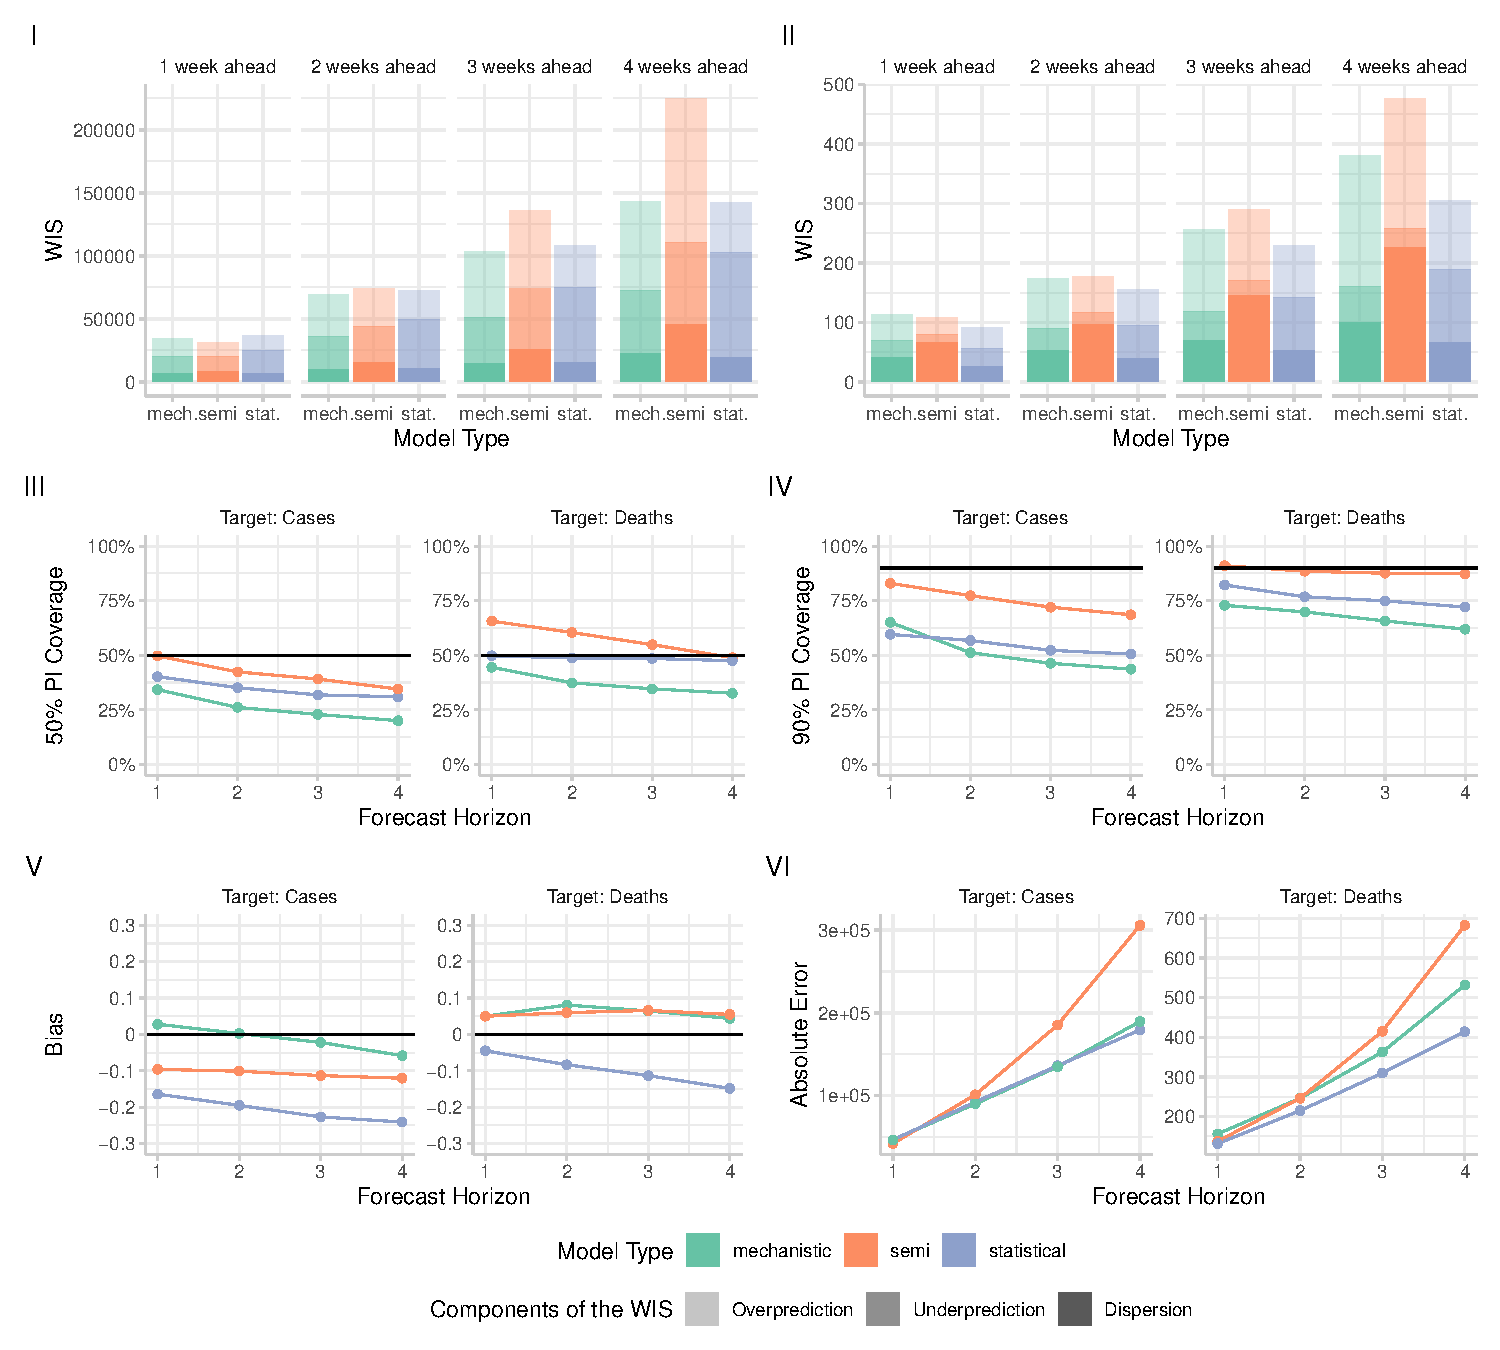
\includegraphics[width = \textwidth]{../plots/overall_assessment_model_types.pdf}
\caption{Performance with respect to several evaluation metrics of the three dominant model types (mechanistic, semi-mechanistic, statistical) in the European Forecast Hub, for two targets (case and death forecasts) and forecast horizons one to four weeks into the future. Results are averaged across five locations, for forecasts made during the time period March 2021 - January 2022. Respectively, the depicted scoring rules / evaluation metrics are: (I), (II) Decomposition of the weighted interval score into overprediction, underprediction, dispersion. (III) Empirical coverage of the $50\%$ prediction interval. (IV) Empirical coverage of the $90\%$ prediction interval. (V) Forecast bias, which ranges between -1 and 1. (VI) absolute error of the median forecasts. Wherever applicable, the desired target value of the score is shown as a black solid line - for all other scoring rules, a lower value of the score corresponds to better performance. Plot heavily inspired by \cite{bosse_comparing_2021-1}.}
\label{fig:decomp_model_types}
\end{figure}\medskip\\ 
\noindent As explained in subsection \ref{ssub:weighted_interval_score}, the weighted interval score can straightforwardly be decomposed into penalties accrued from overprediction, underprediction and dispersion. A question that thus naturally arises is whether the score differences discussed previously can be explained by model types performing particularly well or not with respect to a certain component. To this end, we show the decomposed average WIS obtained by each model type, as well as the absolute error and measures of central interval coverage and bias, in Figure \ref{fig:decomp_model_types}. Note that for the WIS and the absolute error, we report raw average scores rather than scores obtained relative to the baseline model. This is possible since forecasts from all model types are available for the entire time period under study and we first averaged by forecast date and then by model type.\\ 
For the levels of overall WIS in panels (I) and (II), at lower horizons scores in general seem to be varying more between the different forecast horizons than they do between model types, while we once more observe that semi-mechanistic models receive relatively high scores at larger forecast horizons. \\
For forecasting cases, panel (I) shows that this model group receives substantially higher scores from the overprediction component of the WIS at larger horizons, while absolute error (panel (VI)) is also very high. However, according to panel (V), they also show some slight downward bias. Recall that the bias measure, contrary to the WIS, does not scale with the absolute level of the target series and reflects an overall tendency of \textit{relative} under- or overprediction. This thus suggests that as a group, these models actually tend to slightly underpredict case numbers, but then accrue especially high overprediction scores during times of high incidence. Combined with what we discussed previously, that is, the high WIS received during the period with generally highest incidence, this suggests that these models overshot the target during this period, while generally underpredicting during other times. This trend of overshooting during peaks is a behavior that was also described by \cite{bracher_evaluating_2021} for models based on growth rate approaches. A possible reason for this could be that these models are more vulnerable to overprediction at longer horizons, as (slight) overprediction of the growth rate, through the multiplicative nature of the underlying epidemiological process, can lead to large absolute overpredictions of the target.\\
In other cases, the tendency for over- or underprediction as induced by the WIS decomposition and the bias metric are more in agreement. For forecasting deaths, both mechanistic and semi-mechanistic models receive higher scores from the overprediction component than the underprediction component, while also showing very slight upward bias. Conversely, statistical models overall receive higher scores for the underprediction component, while also showing negative bias overall, especially for forecasting cases. \\
%The fact that bias is negative but overprediction component is high, together with their relatively bad performance in period 5, again suggests that these models showed critical overshooting behavior during times of high incidence.\\
%- Lastly, we also see a general result from previous studies: cases get increasingly harder to forecast than deaths at higher forecast horizons.\\
%Furthermore, for both target series, forecasts from semi-mechanistic models receive higher penalties for overdispersion than the other model types.\\
%- consulting overprediction and bias: here we see the ``problem'' with relying on only the overprediction component of the WIS: while semi-mechanistic models get very large scores for overpredicting at longer horizons, the bias metric reveals, suggesting, together with Figure \ref{fig:pw_comp_modeltypes_byperiod}, that the large overprediction score is mostly accrued due to overshooting 
%Interestingly, statistical models more commonly receive penalties for underprediction. It's interesting here to mention that through the multiplicative nature of the underlying epidemiological process, it is often "safer" to score models in terms of underprediction than overprediction in terms of absolute WIS scores.\footnote{We want to pull attention to forthcoming work by Nikos Bosse, who investigates scoring forecasts in terms of relative rather than absolute errors.} \\
Furthermore, Figure \ref{fig:decomp_model_types} shows that semi-mechanistic models tend to be better calibrated, that is, show closer to nominal coverage rates than other model types - this is especially true at the $90\%$ level for both targets, and at the $50\%$ level for case forecasts, while these models are slightly under-confident for death forecasts at the $50\%$ level, where the group of statistical models is almost perfectly calibrated. This shows a common trade-off: as shown by the decomposition of the WIS in panels (I) and (II), semi-mechanistic models lack sharpness for forecasting both target series, but this likely also allows them better coverage, while other model groups issue sharper forecasts at the expense of not containing as many of the observations as they are meant to. As stated in \cite{sherratt_european_2022}, the ensemble in the European Hub suffers from increased overconfidence for Cases with rising forecast horizon on top of general sub-nominal coverage levels, which suggests that these models still might enter favorably into the ensemble by helping to counteract that over-confidence. \cite{bracher_evaluating_2021} made a similar argument for a single component forecast with large dispersion.\\ % Whether this actually holds true, we will investigate further in section XX. 
Generally, we however see a trend of over-confidence for all model types for both targets and furthermore we see a bit of a downward trend in the coverage ratio with rising horizon, especially for case forecasts. This is in line with the general results for component models in the European Hub, as described by \cite{sherratt_european_2022}.
%This is again likely due to the case that ``this group on average'' overpredicts in large absolute terms, particularly in period 5, but in general seems to be somewhat well calibrated (?)...\\
%The only exception seems to be period 3, mostly driven by Great Britain.\\ 
%%%%%%%
\begin{figure}
\centering
\includegraphics[width = \textwidth]{../plots/bl_spread_plot.pdf}
\caption{Two week-ahead forecasts for incidence Deaths in the Czech Republic (I) and incidence cases in Poland (II), for the baseline model as well as four (randomly chosen) component forecasts, during a subset of the period under study that was marked by decline and overall low levels for the respective series. The black line and points show the realized true value of the respective series, while colored lines and points show the forecasts's median prediction, as well as the central $50\%$ and $90\%$ prediction intervals. These plots show that the baseline model, whose confidence bands are based on past differences of the observed series', issues very wide predictive distributions during this period.}
\label{fig:blspread}
\end{figure}\medskip\\ 
We shortly discuss two more general observations that are not directly related to the issue of comparing modeling strategies, but that we nevertheless want to mention. Recall what we previously stated about some periods being easier to forecast in comparison to the baseline: this is especially obvious in period 2 for forecasting deaths, where the series is mostly marked by decline and low levels overall (see Figure \ref{fig:trajectories}) and we observe that all model types markedly outperform the baseline model at virtually all horizons and locations. The consistency of this result across the locations (as well as for some locations for the cases series) led us to investigate the decomposition of the baseline model's WIS during this period. We found that its dispersion component alone sat between 0.96 (at horizon 1) and 1.46 (at horizon 2) of the \textit{overall} average WIS of all other model types, suggesting that the baseline model issued severely under-confident forecasts during this time. Two examples of this behavior are shown in Figure \ref{fig:blspread}, for the deaths series in the Czech Republic in panel (I) and the cases series in Poland in panel (II), where it is evident that the baseline model's predictive distributions are far wider than those of other (randomly chosen) component models.  %\footnote{Does this mean that the baseline model was badly calibrated? Also, find out if this was especially the case during the beginning of a period. Argument could be: baseline not so well adapted to falling numbers, where other models manage to be more confident.} 
Since the baseline model's uncertainty bands are based on past differences, this suggests that these might not update quick enough in such a situation, while all other modeling strategies are generally more capable of issuing more confident forecasts. This marks the point that the choice of baseline is not entirely trivial and that both individual models as well as the more general modeling strategies considered here might appear more capable if only compared to baseline performance during this period. \medskip \\
To see that scores can be heavily dominated by periods and locations with high incidence numbers, consider the results from case forecasts in period 2 in Figure \ref{fig:pw_comp_modeltypes_byloc} and the average in Figure \ref{fig:pw_comp_modeltypes_byperiod}: the semi-mechanistic and mechanistic model type underperforms with respect to the baseline in the aggregate, but they actually markedly outperform the baseline for Poland, Germany and the Czech Republic. Since these countries however have relatively low incidence numbers compared with other countries (France and the U.K.) in the evaluation set during this period (see Figure \ref{fig:trajectories}), they don't influence the average score very much. Put more concretely, the relatively high scores for mechanistic and semi-mechanistic models mostly seem to be driven by their large absolute scores in France. Whether or not this is a desirable feature of the evaluation method is an ongoing debate and can depend on the forecasters' as well as decision makers' preferences. For instance, \cite{bracher_evaluating_2021} argue that scoring forecasts in this manner is meaningful, as a fixed relative deviation from the observed quantity can be regarded as more problematic at high incidence levels rather than at very low incidence levels, which would not be accounted for if only considering the relative deviation. \medskip\\  
Overall, we would conclude from this section that we can't reliably establish a consistent ranking between the three modeling strategies considered here, as all showed periods where they both over- or underperformed with respect to the other strategies (as well as the baseline model), and moreover no clear pattern emerged across the dimensions of the locations or different periods. Furthermore, upon investigation, we often found that variability within these categories was often sizable. Thus, while the modeling strategies are distinct in their approaches and employed toolkits to base short-term forecasts on, it does not seem that one approach is fundamentally better suited than another in our application. On the flip side, this also means that% while there might not exist a dominant overall model type, 
explicit assumptions about the epidemiological process as well as modeling of transmission dynamics don't strictly seem to be necessary for short-term forecasting of COVID-19. In fact, there are many examples of statistical models performing slightly better, for example for forecasting deaths during high-incidence times.\\ 
One somewhat consistent result across the locations considered here (and that was identified previously in \cite{bracher_evaluating_2021}) is the relatively poor performance of the group of semi-mechanistic models during the period with highest incidence, especially at longer horizons. At least for case forecasts, we however must also note here that while this behavior is of course in principle undesirable, forecast performance has generally been found to deteriorate after one or two weeks into the future (both in terms of the WIS and coverage, see e.g. \cite{sherratt_european_2022}), so it might not do well to dwell too much on these differences occurring at longer horizons.\\
An initial goal we had in mind for this analysis was the potential to find patterns across modeling strategies that could be leveraged for ensemble composition - this idea was inspired by an approach by \cite{taylor_combining_2021}, who found that for locations that showed relatively low incidence death numbers, ensembles that purely consisted of mechanistic models outperformed an ensemble that indiscriminately included all component models. While we did not succeed in finding any patterns that are neatly aligned with certain locations or periods of the study, we did observe that substantial differences in performance still occurred at times. In section \ref{sub:weighting_based_on_model_types}, we thus want to investigate whether automatic weighting schemes that are implemented at the level of modeling strategies can provide a boost in performance for the ensemble.
%While we attempted to identify drivers of these scores, we didn't really succeed. Upon further investigation, we generally found that there was considerable variation within the groups and don't feel comfortable making general statements. We however got the idea that, given some of the performance differences over periods in the different locations, it might be possible to devise an ensemble that Thus, we decided to instead do weighting by model types as shown later.\\
%Of course, all of this comes with a caveat. Not really a consistent pattern. Sample size not huge. However, we think that this showed that we can't say that one model type is particularly dominating over another and that in particular, it does not seem that one necessarily needs mechanistic assumptions to model COVID-19.\\
%Limitations: groups are quite small, results somewhat diverge. We are doing this since we are interesting in whether or not one can use this to leverage for the ensemble. As we don't observe any striking patterns, we decide to try automatic weighting by model types-\\
%TO CONCLUDE: NO SYSTEMATIC DIFFERENCES; AND EVEN IF; IT WOULD NOT BE CLEAR WHETHER THIS COULD BE LEVERAGED FOR ENSEMBLE PERFORMANCE: EG BOSSE SHOWS THAT EVEN BAD MODELS CAN BE A GOOD ADDITION TO AN ENSEMBLE: ONE COULD NOW GO AHEAD AND EXCESSIVELY TUNE ENSEMBLE TO SEE IF E:G: SEMI-MECHANISTIC MODELS  WE FELT THAT THE MOST HONEST WAY TO ANALYZE THIS WOULD BE BY AUTOMATIC WEIGHTING: Furthermore, it would be unclear what this would entail in terms of ensemble \\
%IN PARTICULAR; IT IS NOT CLEAR WHETHER PERFORMANCE DIFFERENCES WOULD EVEN MEAN THAT THESE MODELS ENTER UNFAVOURABLY INTO AN ENSEMBLE:
%\subsection{Model Similarity}
%We now turn to the issue of model similarity in ensembles. As expanded upon in Section \todos{XX}, ensemble models are widely regarded to be successful due to the fact that they counteract/mitigate individual model biases and furthermore reduce variance by aggregating a number of models. Regarding the first point of mitigating bias, it is thus conceivable that ensembling approaches could be less successful if some of the included models are too similar. To illustrate this, recall the , thereby skewing 
%include plot of scaled model similarity
%plot of model performance with respect to number of models kicked out
%analyze which models are actually similar 
%This notion has some mention (\todos{find better word}) in the literature. For example, in \cite{bosse_comparing_2021-1}, the authors mention that they purposefully did not submit one of their models for inclusion in the forecast hub's ensemble, as there was concern that it could be too similar to another model they already submitted. However, this decision based on the two models' similarity in modeling setup (shortly explain), rather than on an actual judgment of how close their predictions were. Nevertheless, they did find that both models improved the ensemble if included \todos{(find out if this was actually true)}. We now want to do a more systematic review of this concept - since we will consider more models across more countries, we hope to get a more accurate picture.\\
%\begin{figure}
%\centering
%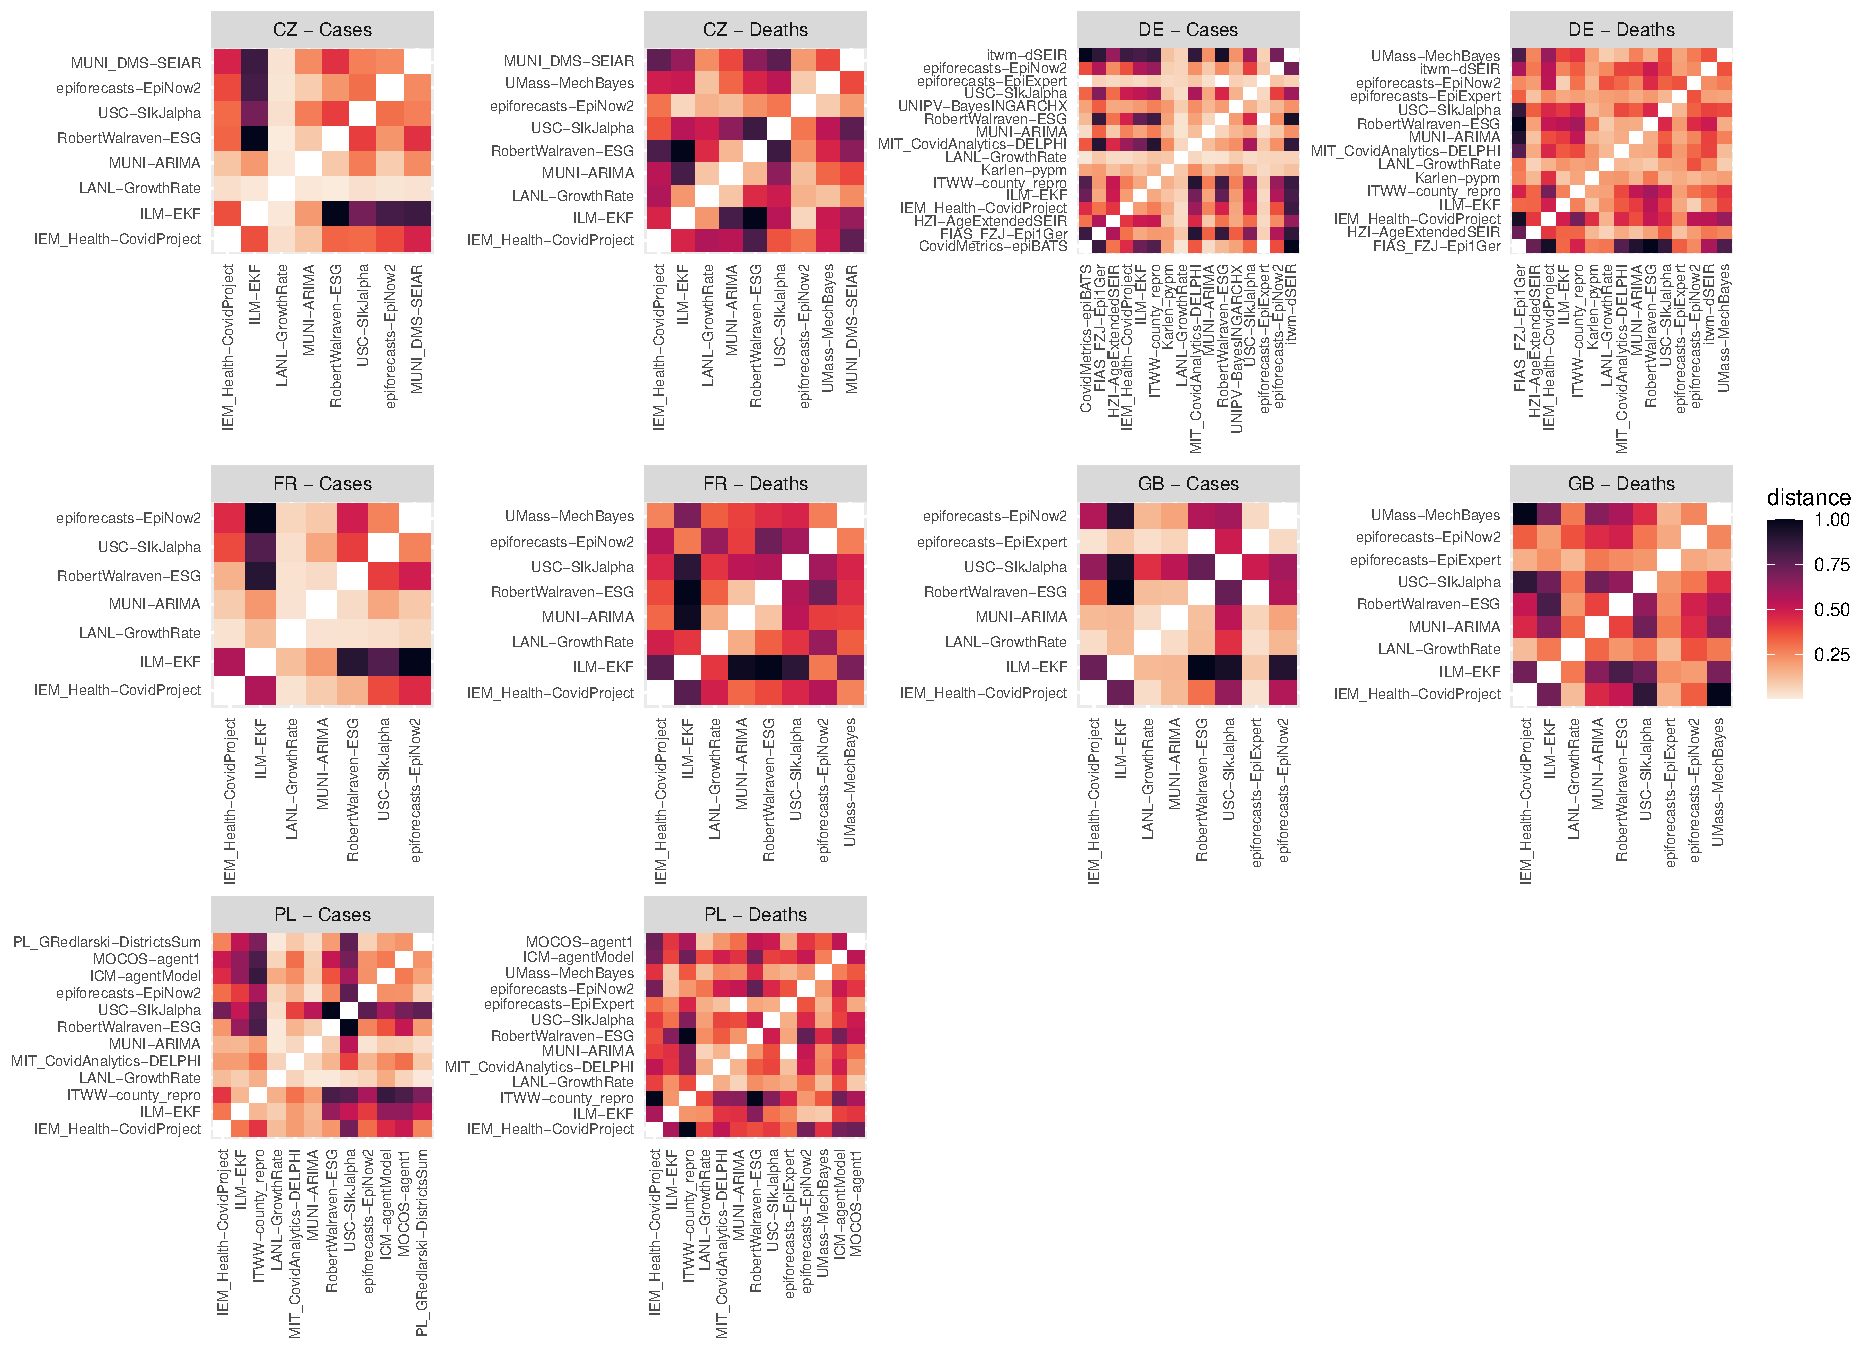
\includegraphics[width = 0.95\textwidth]{../plots/model_similarity.pdf}
%\end{figure}
\subsection{Adding a new model} \label{sub:adding_a_new_model}
%We thus designed the following experiment: for each forecast date, we first built every possible ensemble of size $k$ from the available models at that date. The problem with investigating ensemble size as it relates to performance in the dataset is that, as amply mentioned beforehand, the actual realized ensemble size is not constant as models drop in and out of the Hub, while we also have no universal measure of absolute forecast skill, and one would need to disentangle ensemble size from the inherent level of difficulty present at a given forecast date. In a regression, one could of course control for these idiosyncrasies, but as also mentioned beforehand, scores are not suited as the dependent outcome in a regression and we are furthermore left with the problem of not having a lot of data. But, if we have data on the average score of an ensemble of size $k$, we can study the (expected) added benefit of adding another model to the ensemble. This has some interesting dimensions that we want to explore:\\
While it is a universal result that ensemble models generally exhibit more robust performance than single models, little is known about how individual models can affect an ensemble's performance. This can however be a relevant question: consider the situation where, given an already established ensemble, one is proposed a new model and is consequently confronted with the decision of whether to add it to the base ensemble. The current practice within the Hubs is to include all models that pass a series of data format validity checks - although \cite{ray_challenges_2021} state that forecasters that appeared to be outliers used to be manually removed before the U.S. Hub switched from the mean ensemble to using a median ensemble. However, we believe that this decision of inclusion could presumably be more crucial for smaller base ensembles as they exist in the European Hub, even when using the more robust median ensemble: at larger ensemble sizes, the aggregation function of the ensemble is naturally more robust to single models.\\ 
This question is somewhat inspired by the analysis in \cite{bosse_comparing_2021-1}: they investigated the effect of adding three specific models to the Hub ensemble in Poland and Germany, and found that adding or removing a model induced performance changes that were ``of a similar order of magnitude'' between the mean and median ensemble. Moreover, adding \\ 
  %found that performance changes from adding or removing a model from the ensemble were ``of a similar order of magnitude, suggesting that at least in this instance, with a relatively small ensemble size, the median ensemble was not necessarily more ``robust'' to changes than the mean ensemble''.
There are several different lines of inquiry that thus arise with respect to this question. First of all, it is interesting to consider whether it is more ``safe'' to add a model during certain periods more than others, especially for periods with higher incidence levels. Furthermore, effects might be different based on the type of model added to the ensemble, with regard to models being better or worse performers or more or less distant to the base ensemble. Lastly, all of these effects might be different for the mean and median ensemble. \\
%We investigate these questions via two characterizations of the proposed model: its recent performance as well as its distance to the base ensemble, as measured by the Cramer distance. The latter is always in the information set at the forecast origin, as it is simply a measure of distance between the issued predictive distributions. To assess the former, one needs at least a small historical record of the proposed model's performance.\\
Concretely, we decided that the most systematic path to investigate this question was via first building counterfactual ensembles - that is, at each of the available forecast dates, we recombined the set of available models into all possible sets of size $k$, which we subsequently combined into an equally weighted mean and an equally weighted median ensemble. We believe these ``alternative ensembles'' and their corresponding performance to be valid counterfactuals, as we generally believe that participation of one model at a given forecast date is independent of that of another. We thus obtain a large sample of alternative ensembles with constant size over time, thus allowing us to keep ensemble size constant while investigating other effects.\\ 
Based on these data, we then designed the following experiment: we took a random sample of size 100 from all possible ensembles with $k$ member models at each forecast date, location and for each of the target series. For $k$, we decided to investigate a relatively small base ensemble size of $k = 4$ as well as a more moderate size of $k = 8$. Due to the differences in model availability, the latter setting was only viable for Germany an Poland.
\begin{figure}
\centering
\includegraphics[width = 0.82\textwidth]{../plots/add_model_boxplot}
\caption{Distribution of scaled WIS after adding different types of models from a proposed set of four models to base ensembles with four (I) and eight (II) member models. Models were added based on the characteristics: best/worst performer, minimum/maximum distance to the base ensemble and a reference (randomly chosen) model. The WIS after adding the respective model was scaled by the WIS of the base ensemble beforehand, as a measure of change in performance resulting from adding the respective model. Outlying values $>$ 2 are excluded from the plots, and the mean values of the scaled WIS (indicated in black) are included to account for this.}
\label{fig:spread_gamma}
\end{figure}\\
For each of these base ensembles, we proposed four of the remaining component forecasts as new members for the ensemble. We deliberately kept the number of proposed models constant as we did not want to skew results by fluctuations in model availability over time.\footnote{Although we still had to exclude a few forecast dates for some locations where model availability was too low.} From this set of proposed models, we added both the best and worst recent performer (as judged by the relative WIS obtained on the as of the particular forecast date resolved forecasts of the past four weeks), as well as the model with the largest as well as smallest distance to the current ensemble. Finally, we also added a random model from the set, as a reference to compare the resulting effects against. All of the resulting ensembles were subsequently scored via the WIS and scaled by the base ensemble's score. We thereby get a direct measure of the change in performance as a consequence of adding the respective model.\\
%Since the median is the aggregation method used in most applications for forecasting COVID-19, this suggests
%We want to make a first step in this direction by studying the effect that \textit{adding} another model will have on an ensemble.  In particular, we want to study whether any model is indiscriminitaly a good addition to an ensemble, or whether we can identify differences across 
%- are there times (high vs. low incidence is what most easily comes to mind) where adding a model is more beneficial?\\
%- is adding a model more beneficial for the mean or the median ensemble? \cite{bosse_comparing_2021-1} found that performance changes from adding or removing a model from the ensemble were ``of a similar order of magnitude, suggesting that at least in this instance, with a relatively small ensemble size, the median ensemble was not necessarily more ``robust'' to changes than the mean ensemble''. They find also that adding a 
%- are there differences between adding a model that is more vs less distant to the current ensemble?
%- how much does individual model performance matter? How "safe" is it to add any model, even if it might be a bad performer?  
%- are there models that if added provide a particularly good benefit?\\
%We see that adding a very close model has almost no impact on the mean ensemble, while it does move the median ensemble. Since the median is a more discrete measure, its predictions are more skewed by adding another model. \\
%One can of course argue that one is usually more interested in the median effect of adding another model. The following can thus be regarded as an analysis on how ``safe'' it is to add a certain model and in certain situations.\\ 
%Of course, this has the downside of limiting the maximum ensemble size that can be studied. This can better enhance understanding of ensemble behavior. To our knowledge, such an experiment is novel in the literature. 
We did this separately for the two ensemble types - note thus that the model added based on distance to the base ensemble was not necessarily the same for the mean and median ensemble, although we found that it was in most cases (e.g. for $k = 4$, there was an agreement of $76.5\%$ for the minimum and $88.3\%$ for the maximum distance model and for $k = 8$, an agreement of $72.2\%$ for the minimum and $83.5\%$ for the maximum distance model). We regard this as more of a sanity check of our implementation, as we would expect the mean and median model to generally be closer to one another than to any component forecast and hence be closest to and (in particular) most distant to the same model. Conversely, the identity of the best or worst recent performer only depends on the set of proposed models, hence the model added based on the performance measure was always the same, regardless of ensemble type.\\
% latex table generated in R 4.2.0 by xtable 1.8-4 package
% Wed Sep  7 13:03:20 2022
Figure \ref{fig:spread_gamma} shows the distribution of relative scores, separately for the two target series, the different types of models added and the type of base ensemble. For both sizes of the base ensemble, the median relative scores for all added models tend to be closely below one, meaning that it was beneficial to add another model in most cases, irrespective of that model's nature, the target series or the type of base ensemble. Furthermore, differences in the spread of relative scores between the two target series are overall not apparent. \\
Median and average relative scores for the best model are usually a bit lower than those of the worst and the random model, suggesting that there may be some benefit in selecting for better recent performers.\\
Considering overall differences in variation between models for the mean ensemble, these are somewhat more pronounced: especially for $k = 4$, the maximum distance model is associated with a larger spread in scores, compared to the minimum distance model, which overall has little effect on performance. Furthermore, the median and average scores diverge substantially for the maximum distance model, suggesting that adding a model with large distance to a mean ensemble is simultaneously quite beneficial in most cases and can have large detrimental effects in others. Conversely, spreads in scores are overall more similar for the median ensemble, with only a slightly larger variation in scores for the maximum distance model.\\
Pertaining to differences with respect to the size of the base ensemble, spread in relative scores is consistently reduced for the larger setting, supporting our previous point that the performance of ensembles that already contain a larger number of component models becomes more robust to newly added ones of any nature. \medskip\\
While the median relative scores thus mostly stay close below one, mean relative scores are often substantially higher. One could argue that these mean effects are also of considerable interest, as they give a more accurate picture of how ``safe'' it is to add a model to an ensemble. With the relative scores generated here, single outliers are less of an issue, measurements are not systematically correlated and the data set is considerably larger than in the original data set with direct absolute scores. We thus felt it was viable to fit a generalized linear model - as we observed the conditional distributions of the outcome to be positively skewed and as relative scores are restricted to the positive real line, the natural choice was to model scores via 
%Due to the fact that we are thus dealing with relative rather than absolute scores, which are not as affected by large outliers, and the large size of the data we generated, we felt it reasonable to run a regression analysis. \todos{write something about independence of measurements: resampling, not the same model all the time, equally hard to score relatively well.} 
%As we noticed the conditional distribution of the relative scores to still be right skewed and since relative scores are restricted to the positive real line, we decided to model the scores via 
the two parameter gamma distribution as it is implemented in the \texttt{gamlss} package \citep{rigby_generalized_2005}. This particular implementation models the distribution via two parameters, $\mu$ and $\sigma$, with $\mu$ the mean of the response and $\sigma^2$ the dispersion\footnote{Not to be confused with the dispersion component of the WIS.} parameter. The distribution's standard deviation linearly scales with the $\sigma$-parameter (which is modeled via a log-link function), meaning that a negative sign of an estimate for the $\sigma$-parameter corresponds to a ceteris paribus decrease of the standard deviation of the response. While it is not straightforward to interpret the size of the resulting coefficients, we can analyze whether the effects are of similar orders of magnitude for the different models and ensemble types.\\
Hence, we fit a regression of the relative score on the type of model that was added to the ensemble (best/worst recent performer; minimum/maximum distance), with the randomly added model as a reference category, separately for the two ensemble types. We additionally included the forecast horizon as a predictor, as well as random effect terms for the interaction of location, target series and the periods as defined in section \ref{sub:hub_data}, to control for idiosyncrasies that might have arisen at certain location - time combinations of the respective target series.
\input{tables/gamma_results_nmod4.tex}\\
The resulting coefficients, as well as their standard errors, for $k = 4$ are reported in Table \ref{tab:gamma_results_nmod4}.\footnote{We refrain from explicitly marking the significance, as all estimates are highly significant. Due to the large sample we created (n = 535980) through the recombination experiment, we would argue that the concept of significance is not that meaningful here.} Pertaining to the recent performance of the added model, it can be observed for both ensemble types that this does have an effect on the average relative performance: adding a model that has shown good relative performance in the near future leading up to the forecast date on average improves performance more than a random choice of model, while adding a model that has performed relatively poorly also leads on average to a worse performance of the ensemble. In regards to the differences between the two ensemble types, we note that the effects for the mean are larger - moreover, the effects on the dispersion (and thus the variance) of the relative scores are substantially larger for the mean ensemble. This is likely due to the fact that the mean ensemble is more vulnerable to outliers - it thus seems to be the fact that it is particularly ``safe'' to select an additional model based on recent performance for the mean ensemble, compared to adding a random model. \\%The performance characteristic thus seems to be a more important selector for the mean ensemble, while for the median ensemble it overall does not matter as much what model is added.\\
For both ensemble types, variance of the relative scores is reduced when adding a model that is particularly similar to the established ensemble, compared to adding a random model. This is likely also exacerbated by the relatively small ensemble size we are considering here - at only four component models in the ensemble, adding another model can in principle greatly move the ensemble's predictions (and thus impact its performance). Adding a model that is more in agreement with the established ensemble thus leads to less of a spread in relative scores, while adding one that ``disagrees'' with will have larger impact. In theory, this could also mean that there is more potential for improvement. However, especially for the mean ensemble, adding a model with larger distance is also associated with an expected increase in scores, compared to simply adding a random model. When interest thus lies in stability, care should be taken when considering an additional model that is in disagreement with the current ensemble.\\
Furthermore, across the board, we observe that effects are larger for the mean ensemble, for both the mean and the dispersion parameter. This again supports the statement that the mean ensemble is moved more easily by an additional model and is in particular more vulnerable to outlying forecasts. \\
For the horizon effect, we generally see that 
\input{tables/gamma_results_nmod4_plde.tex}\\
We expected that the size of these effects would be bigger if we had more models to choose from, as the choice of a model based on both performance and distance measures becomes more meaningful if the set of models it is chosen from is larger. To check this, we reran the analysis for only Poland and Germany and consequently were able to propose two more models at each forecast date. The results are reported in Table \ref{tab:gamma_results_nmod4_plde}, where we see that most effects are larger in the absolute, for both the mean and the dispersion parameter. In particular, the effects for the maximum distance model are increased. This suggests that the further a proposed model is from the base ensemble, the greater the risk for large deterioration in performance, compared to adding a random reference model. Effects on the mean and dispersion of the relative scores also increase in the absolute for the performance based models, suggesting that the better (or worse) a forecast model has performed in recent times, the safer (or riskier) it is to add to an ensemble.\\
Lastly, we report the regression results for the larger base ensembles ($k = 8$) in Table \ref{tab:gamma_results_nmod8}. In congruence with the reduction of variation in the aggregate relative scores that we discussed earlier, effect sizes are reduced for these larger ensembles. Nevertheless, the addition of the worst and maximum distance model still impact the average relative score, particularly for the mean ensemble. This suggests that at such an ensemble size, which is not uncommon for some countries in our set as well as other countries in the European Hub, ensembles can still be somewhat vulnerable to such additions. Note also that the intercepts for the mean parameter are reduced, reflecting the fact that adding any model becomes safer for a larger ensemble.
%An interesting observation that arises in all regression specifications is that the intercept is smaller in absolute terms , meaning that the dispersion of the relative score distributions is generally larger for the median ensemble. We think this might be due to the fact that the median is a more discrete measure and is thus more easily moved by any addition. Put differently, at smaller ensemble sizes, the median ensemble is more easily moved by any addition, but is simply more robust to the type of model that is added.
\input{tables/gamma_results_nmod8}
\begin{figure}
\centering
\includegraphics[width = \textwidth]{../plots/gamma_reg_random_effects_nmod4
}
\caption{Fitted random effects for the mean parameter from a generalized regression with gamma distributed response. The response variable is the relative score that results after adding a model to a base ensemble with four member models, using the median (I) or mean (II) as the aggregation function. The base ensembles were recombined from the set of available forecast models in the data at each forecast date, separately for the different target series and locations.}
\label{fig:replots}
\end{figure}\\
Considering the question of whether it is in general safer/riskier to add models to an ensemble depending on the phase of the epidemic, we additionally show the fitted random effects from the model in Table \ref{tab:gamma_results_nmod4}, in Figure \ref{fig:replots}. The effects were contrast-coded, and thus represent deviations from the overall intercept. While variation between locations for a given period is somewhat pronounced for both target series, effects for the median ensemble (panel (I)) are overall more similar. For the mean ensemble (panel (II)) effects vary more and tend to be larger during the period with highest incidence, especially for the cases series. This could be due to the fact that models in general issue more varying predictions during these periods of higher incidence, especially for the cases series. This effect can also be observed for the median ensemble, albeit to a lesser degree, once more supporting the point that the median ensemble is more resistant to additions. For the setting with the larger base ensemble, variation in random effect sizes was substantially less pronounced, again supporting the point that larger ensembles become more robust (Appendix, Figure \ref{fig:replot_nmod8}).\medskip\\ 
Finally, while it emerged that adding another model will improve an ensemble's scores in most cases, our analysis also suggests that due to potentially large deteriorations in the relative score, care should be taken when adding a new model to an existing ensemble, especially when that model has shown poor performance in recent weeks or it is in disagreement with the current ensemble. When confronted with such a decision, it might be wise to manually check such a forecast model for plausibility - that is, whether e.g. its distance from the current ensemble could result from a data error. It could also be beneficial to assess the performance of the current ensemble in recent weeks and appraise whether the proposed model could somehow ``correct'' undesirable characteristics of the ensemble - for instance, \cite{bosse_comparing_2021} identified a case where a poorly performing model nevertheless improved the overall ensemble, as it was more ``directionally correct'' relative to it. However, as the overall decrease in effect sizes for the larger base ensemble suggests, we would expect that at yet larger ensemble sizes (which we could not feasibly consider given our limited model base), ensembles are likely sufficiently robust to single models, such that manual screening of models might not be that beneficial.\\
Lastly, our results once more suggest that the median is the more robust choice as an aggregation function for the ensemble, especially at the rather low to moderate number of member models we have considered here.\\
Admittedly, the analysis performed in this section was to a degree stylized. Nevertheless, this experiment allowed us to support some previously held intuitions, namely that both the recent performance of a model as well as its disagreement with the current ensemble can impact the performance of the ensemble it is a member of. However, while differences were noticeable both between the types of added models and the type of base ensemble, it is difficult to judge how meaningful the differences in effect sizes are. In the next section, we thus want to investigate whether ``reverse-engineering'' these results by consistently selecting for better performers is a reasonable strategy.\\
%Lastly, we acknowledge that this analysis has a certain stylized character. During the next section, we especially 
%These ``hypothetical ensembles'' we believe to be valid counterfactuals, as it could have easily been the case that e.g. one forecaster dropped out due to e.g. technical issues.\\
%To conclude, we would again argue that 
%%%%%%%%%%%%%%%%%%%%%%%%%%%%%%%%%%%%%%%%%%%%%%%%%%%%%%%%%%%%%%%%%%%%%%%%%%%%%%%%%%%%%%%%%%%%%%%%%%
%%%%%%%%%%%%%%%%%%%%%%%%%%%%%%%%%%%%%%%%%%%%%%%%%%%%%%%%%%%%%%%%%%%%%%%%%%%%%%%%%%%%%%%%%%%%%%%%%%
%%%%%%%%%%%%%%%%%%%%%%%%%%%%%%%%%%%%%%%%%%%%%%%%%%%%%%%%%%%%%%%%%%%%%%%%%%%%%%%%%%%%%%%%%%%%%%%%%%
%%%%%%%%%%%%%%%%%%%%%%%%%%%%%%%%%%%%%%%%%%%%%%%%%%%%%%%%%%%%%%%%%%%%%%%%%%%%%%%%%%%%%%%%%%%%%%%%%%e
%%%%%%%%%%%%%%%%%%%%%%%%%%%%%%%%%%%%%%%%%%%%%%%%%%%%%%%%%%%%%%%%%%%%%%%%%%%%%%%%%%%%%%%%%%%%%%%%%%
%%%%%%%%%%%%%%%%%%%%%%%%%%%%%%%%%%%%%%%%%%%%%%%%%%%%%%%%%%%%%%%%%%%%%%%%%%%%%%%%%%%%%%%%%%%%%%%%%%
%%%%%%%%%%%%%%%%%%%%%%%%%%%%%%%%%%%%%%%%%%%%%%%%%%%%%%%%%%%%%%%%%%%%%%%%%%%%%%%%%%%%%%%%%%%%%%%%%%
%%%%%%%%%%%%%%%%%%%%%%%%%%%%%%%%%%%%%%%%%%%%%%%%%%%%%%%%%%%%%%%%%%%%%%%%%%%%%%%%%%%%%%%%%%%%%%%%%%
\newpage
\section{Ensemble Experiments}
Some of these techniques came up . We thus retroactively analyze other ensembling methods. In light of the fact that . One could in theory denote a holdout set, but given the fast changes in disease characteristics, the periods are not really comparable.\\ 
While this is a retroactive analysis, it is generally important that it, to the extent that it is possible, simulates the real-time. That is, only information that is available up to that point in time may be used for building the ensemble. This is because we want to trial (and if successful, suggest) methods that in theory could be deployed in real-time. Otherwise, it would be too easy to retroactively devise strategies that outperform the ensemble.\\
Generally, for all "ensemble experiments", the sets of models that would enter the ensemble were automatically stratified by target type, location and of course the forecast date. Theoretically, one could also stratify by horizon.\footnote{Or even quantile? As done by US hub in ensemble experiments.} The reasoning for this is clear: some models or model types might be better at forecasting certain horizons than others. However, this could lead to things going entirely haywire \\
Note that we refrained from excessively tuning hyperparameters in the study.
We wanted to derive methods that accounted for the fact that weight estimation does not work well in low signal-to-noise ratio settings \cite{claeskens_forecast_2016}.\\
%We decided to implement an ensemble that is based on the results from 1, i.e. that namely excludes semi-mechanistic models at longer horizons. Of course, we also saw that mechanistic models had rather poor performance at longer horizons, but we decided to exclude only semi-mechanistic as we otherwise wouldn't have much of an ensemble left at all. Furthermore, while the trend isn't $100\%$ clear, we mostly see that semi-mechanistic models perform either second-worst or worst. Also, while we identified a general tendency for larger dispersion (which might actually aid the generally overconfident ensemble), we additionally at larger horizons saw a much more problematic tendency to overpredict the target. We will do this analysis for both cases and deaths, but of course expect larger benefits for case forecasts. Compared with both the relative scores of the other model types, we see that semi-mechanistic models are rarely a good performer when compared to the other model types.  We of course expect this to improve performance in-sample, but further we want to investigate whether this introduces any unwanted effects, i.e. discontinuities. Namely, there are a few desirable properties of forecasts that could be in jeopardy if the set of models in the ensemble varies with the forecast horizon. It is thus conceivable that these models increase the cone of uncertainty for lower horizons, making it drop afterwards if they are then excluded. Furthermore, we also monitor the resultant coverage of the ensemble before and after, to see if anything worsened in this regard - wis might drop (not a surprise, as this is how it was selected), but that makes monitoring other scoring rules even more important. \\
For evaluation, we use a more direct relative WIS, since there are no missing forecasts in this part of the analysis.\\
Our analyses in the previous sections showed some (if slight) performance differences of  \\
Lastly, we chose to compare our methods to an ensemble that employed the unweighted median over the entire study period rather than the actualized Hub ensemble. This is due to the aforementioned fact that the Hub changed their aggregation method from mean to median in July(?) of 2021. We noticed that in the aggregate (that is, over the entire study period), some of our methods, most notably those based on the weighted median, compared favorably to the actualized Hub ensemble, which however mostly stemmed from the early months of 2021. We felt that this was somehow misleading, so instead opted to use the median ensemble as a benchmark throughout the study period. We checked that our ensembling method gave similar predictions to the hub ensemble. Whenever we refer to the ``benchmark'' model during this section, we are thus referring to the equally weighted median ensemble that indiscriminately includes all models. Whenever we refer to aggregate performance, we refer to .... \\
%\subsection{Model Types}
%These compartmental models, via a set of differential equations, explicitly model how members of the population transition through the states of being susceptible, (exposed), infected, and recovered/removed \cite{taylor_combining_2021}.
\subsection{Best performers} \label{sub:best_performers}
In this section, we investigate whether changing the model base such that only the recent best performers are included in the ensemble, potentially in conjunction with additionally weighting component forecasts based on past performance, can improve performance relative to the equally weighted median ensemble that indiscriminately includes all models. We have several reasons why we believe this approach could prove fruitful. \medskip\\
%%%%%%
First of all, this approach has some precedence in the U.S. Hub: \cite{ray_comparing_2022} find that a combination method that simultaneously reduces the model set to the ten recent best performers and subsequently weights these by their past performance (in terms of the relative WIS) performs consistently better than an equally weighted median for forecasting deaths, while it does not work better for forecasting cases. As a consequence, the relative WIS weighted median ensemble superseded the equally weighted median ensemble as the U.S. Hub's official method for forecasting deaths in November 2021.\\ 
In fact, they state that they also applied this method to the European Hub, where the method however showed worse performance relative to the equally weighted median including all component forecasts, for both deaths and cases. This could however be due to the substantial differences in model availability between the two Hubs - as previously stated, most models participating in the U.S. effort submit forecast for all locations (that is, states), while this is only the case for less than half the models in the European Hub. Since their method only selects the best ten models measured by relative WIS across the entire European set, we surmise that it could fail due to two reasons.\\
First of all, the approach in effect substantially reduces the model set for most locations, as it will likely select some models which only submit forecasts for a small number of locations or even just a single location - recall our finding in section \ref{sub:model_types_analysis} that found that Poland's agent-based models had substantially lower relative WIS than other model types, at least for forecasting cases. This way of selecting models presumably already leads to worse performance due to the sheer effect of greatly reducing ensemble size at some locations, and potential benefits of the method would thus not get a chance to properly unfold.\\
Second of all, we noticed during our investigations of the data that a model that is a good performer for one location at a given time isn't necessarily one for all other locations. Moreover, when using the WIS to judge component forecasts, we could have the case that locations with nominally high levels of incidence could, in a sense, dictate the model set for all locations. We thus believe that it's better to allow stratification by location, even though it could also make the approach more vulnerable to variations in single models' performance. \\
Hence, we will investigate whether an approach of treating each location's model set separately can improve performance, as it ensures that each location is given a full set of best $k$ performers unique to that location. Nevertheless, we are still dealing with the aforementioned issue that the model base is not large to begin with, so even when attempting to draw from the available resources as much as possible, reducing ensemble size further could counteract any potential benefits from choosing better performers, as the ensemble in theory becomes more vulnerable to failure or erratic behavior of single component forecasts if the number of models is small. \medskip\\%Fundamentally, the better we are  This is due to the fact that individual performance can be erratic and past performance is not a perfect predictor to recent performance. \\
Second of all, \cite{sherratt_european_2022} showed that for the European Hub, employing a weighting scheme where all models are weighted based on their past performance did not provide a benefit over the equally weighted median, neither when subsequently using a weighted mean or weighted median. The question thus remains whether either pure model selection or combining weighting with prior selection of recent good performers could provide a benefit. In the case where it is possible to identify models that truly have an edge over others, it might be beneficial to reduce the model set to these models, whether or not they are subsequently weighted, as estimating weights for all models could be too noisy.\\ %We however don't expect good results from weighting, as we believe that estimating weights in a reduced model set could actually be detrimental in a situation where noise is high (model performance generally varies a lot). We rather expect a strict reduction of the model set, which effectively amounts to setting all other weights to zero, to perform better. The rationale behind this approach is that it is to a certain degree less flexible than choosing true weights, i.e. a sort of shrinkage method (similar to LASSO). However, this could only work if consistent performers exist and they can reliably be identified. \todos{maybe better: just give arguments for both approaches without saying which one is better}. Considering just selection or selection with weighting: in case there is signal and not just noise it might be good to weight.\\
Lastly, our results in section \ref{sub:adding_a_new_model} showed that adding a relatively good performer on average has a better effect on the ensemble, compared with the addition of a ``random'' model. We thus want to study whether this can, somehow, be ``reverse-engineered'' and whether it can be beneficial to purposefully tune the set of models such that ``random'' models are kicked out and only the relatively good performers remain. Note that here the procedure is different to what we did in section \ref{sub:adding_a_new_model}: we are actively removing models from the set, while before we investigated the effect of adding a model to the ensemble. While these are to a certain degree just two sides of the same coin, in practice - due to the expected gains in ensemble performance when adding any model - an ensemble builder is more realistically faced with the decision of removing a model from the existing model base rather than adding an extra model to it. \medskip \\ %However, since we did observe some differences in adding models based on, we want to investigate whether this can also be applied to the practice retroactively selecting models.  \medskip \\
We thus proceeded as follows. At each forecast date, via a rolling window of the respective past four weeks, we select the number of $k$ models with lowest relative WIS within that window. If one of the selected models did not participate at the current date, the next best model takes its place - put differently, we only select from the set of models that are actually available at the current date, to ensure that ensemble size is always constant. Forecasts that have not resolved yet by the respective forecast date are excluded from scoring, since the resolution of, for instance, the most recent 3-week forecast would not be in the information set of the ensemble forecaster in a real-time setting, which we want to mimic as closely as possible. The set of scored targets thus includes one 4-week ahead forecast, two 3-week ahead forecasts, three 2-week ahead forecasts and four 1-week ahead forecasts.\\
In principle, the window size is of course a tuning parameter that can affect the results. Given that our analysis is entirely retrospective, we refrained from excessively tuning this parameter to the point where it would give the most favorable in-sample results. We therefore chose a similar value to the one used by \cite{bracher_pre-registered_2021} in a related analysis - they used a window size of three weeks to estimate weights, which we slightly increased to four weeks as we wanted to include at least one forecast from all horizons. In theory, this parameter can be seen as a dial between the bias and variance of estimating model weights: in so far as average model performance is not stationary, bias decreases if we use less recent observations, while variance increases (due to random fluctuations in model performance having more effect on the weights). We believe that four weeks strikes a good balance between the two. \\%We however also mention that in practice, \cite{ray_comparing_2022}, who use a window of 12 weeks, state that they did not observe substantial differences when varying this parameter.\\
%For this approach, we scored models based on their performance in the past four weeks. To assess this performance, we only scored forecasts that had resolved by the current forecast date, in order to better mimic the real-time situation. This means that we excluded forecasts if they were made before the current date, but for a horizon that as yet lay in the future relative to the current date. \\ 
To mitigate the recently mentioned issue of varying model base, we score models and thus construct the best performers set separately for each location, as well as separately for the two series. Within the window of four weeks, we allowed models at most one missing forecast, otherwise they were not considered for selection. This is the reason we chose to use the relative WIS rather than the average score obtained by each model, since, as amply mentioned beforehand, the average score can be heavily influenced by single targets that were particularly hard to forecast and thus induced large absolute scores. Models that missed forecasting this particular target could thus receive a relatively low average score and as a consequence undeservedly be included in the best performers set.\\
As an aggregation method for the thereby induced sets of best recent performers, we considered the equally weighted median, the equally weighted mean, as well as a weighted approach for both. For the weighted methods, we employed inverse score weighting as detailed in section \ref{sub:ensemble_techniques}. In the cases where component forecasts had missed one target within the current window used to estimate the weights, we proceeded as in \cite{bracher_pre-registered_2021} and imputed that past score with the worst score achieved by any model for that particular target.%equally weighted median ensemble constructed from the full available model base
\begin{figure}
\centering
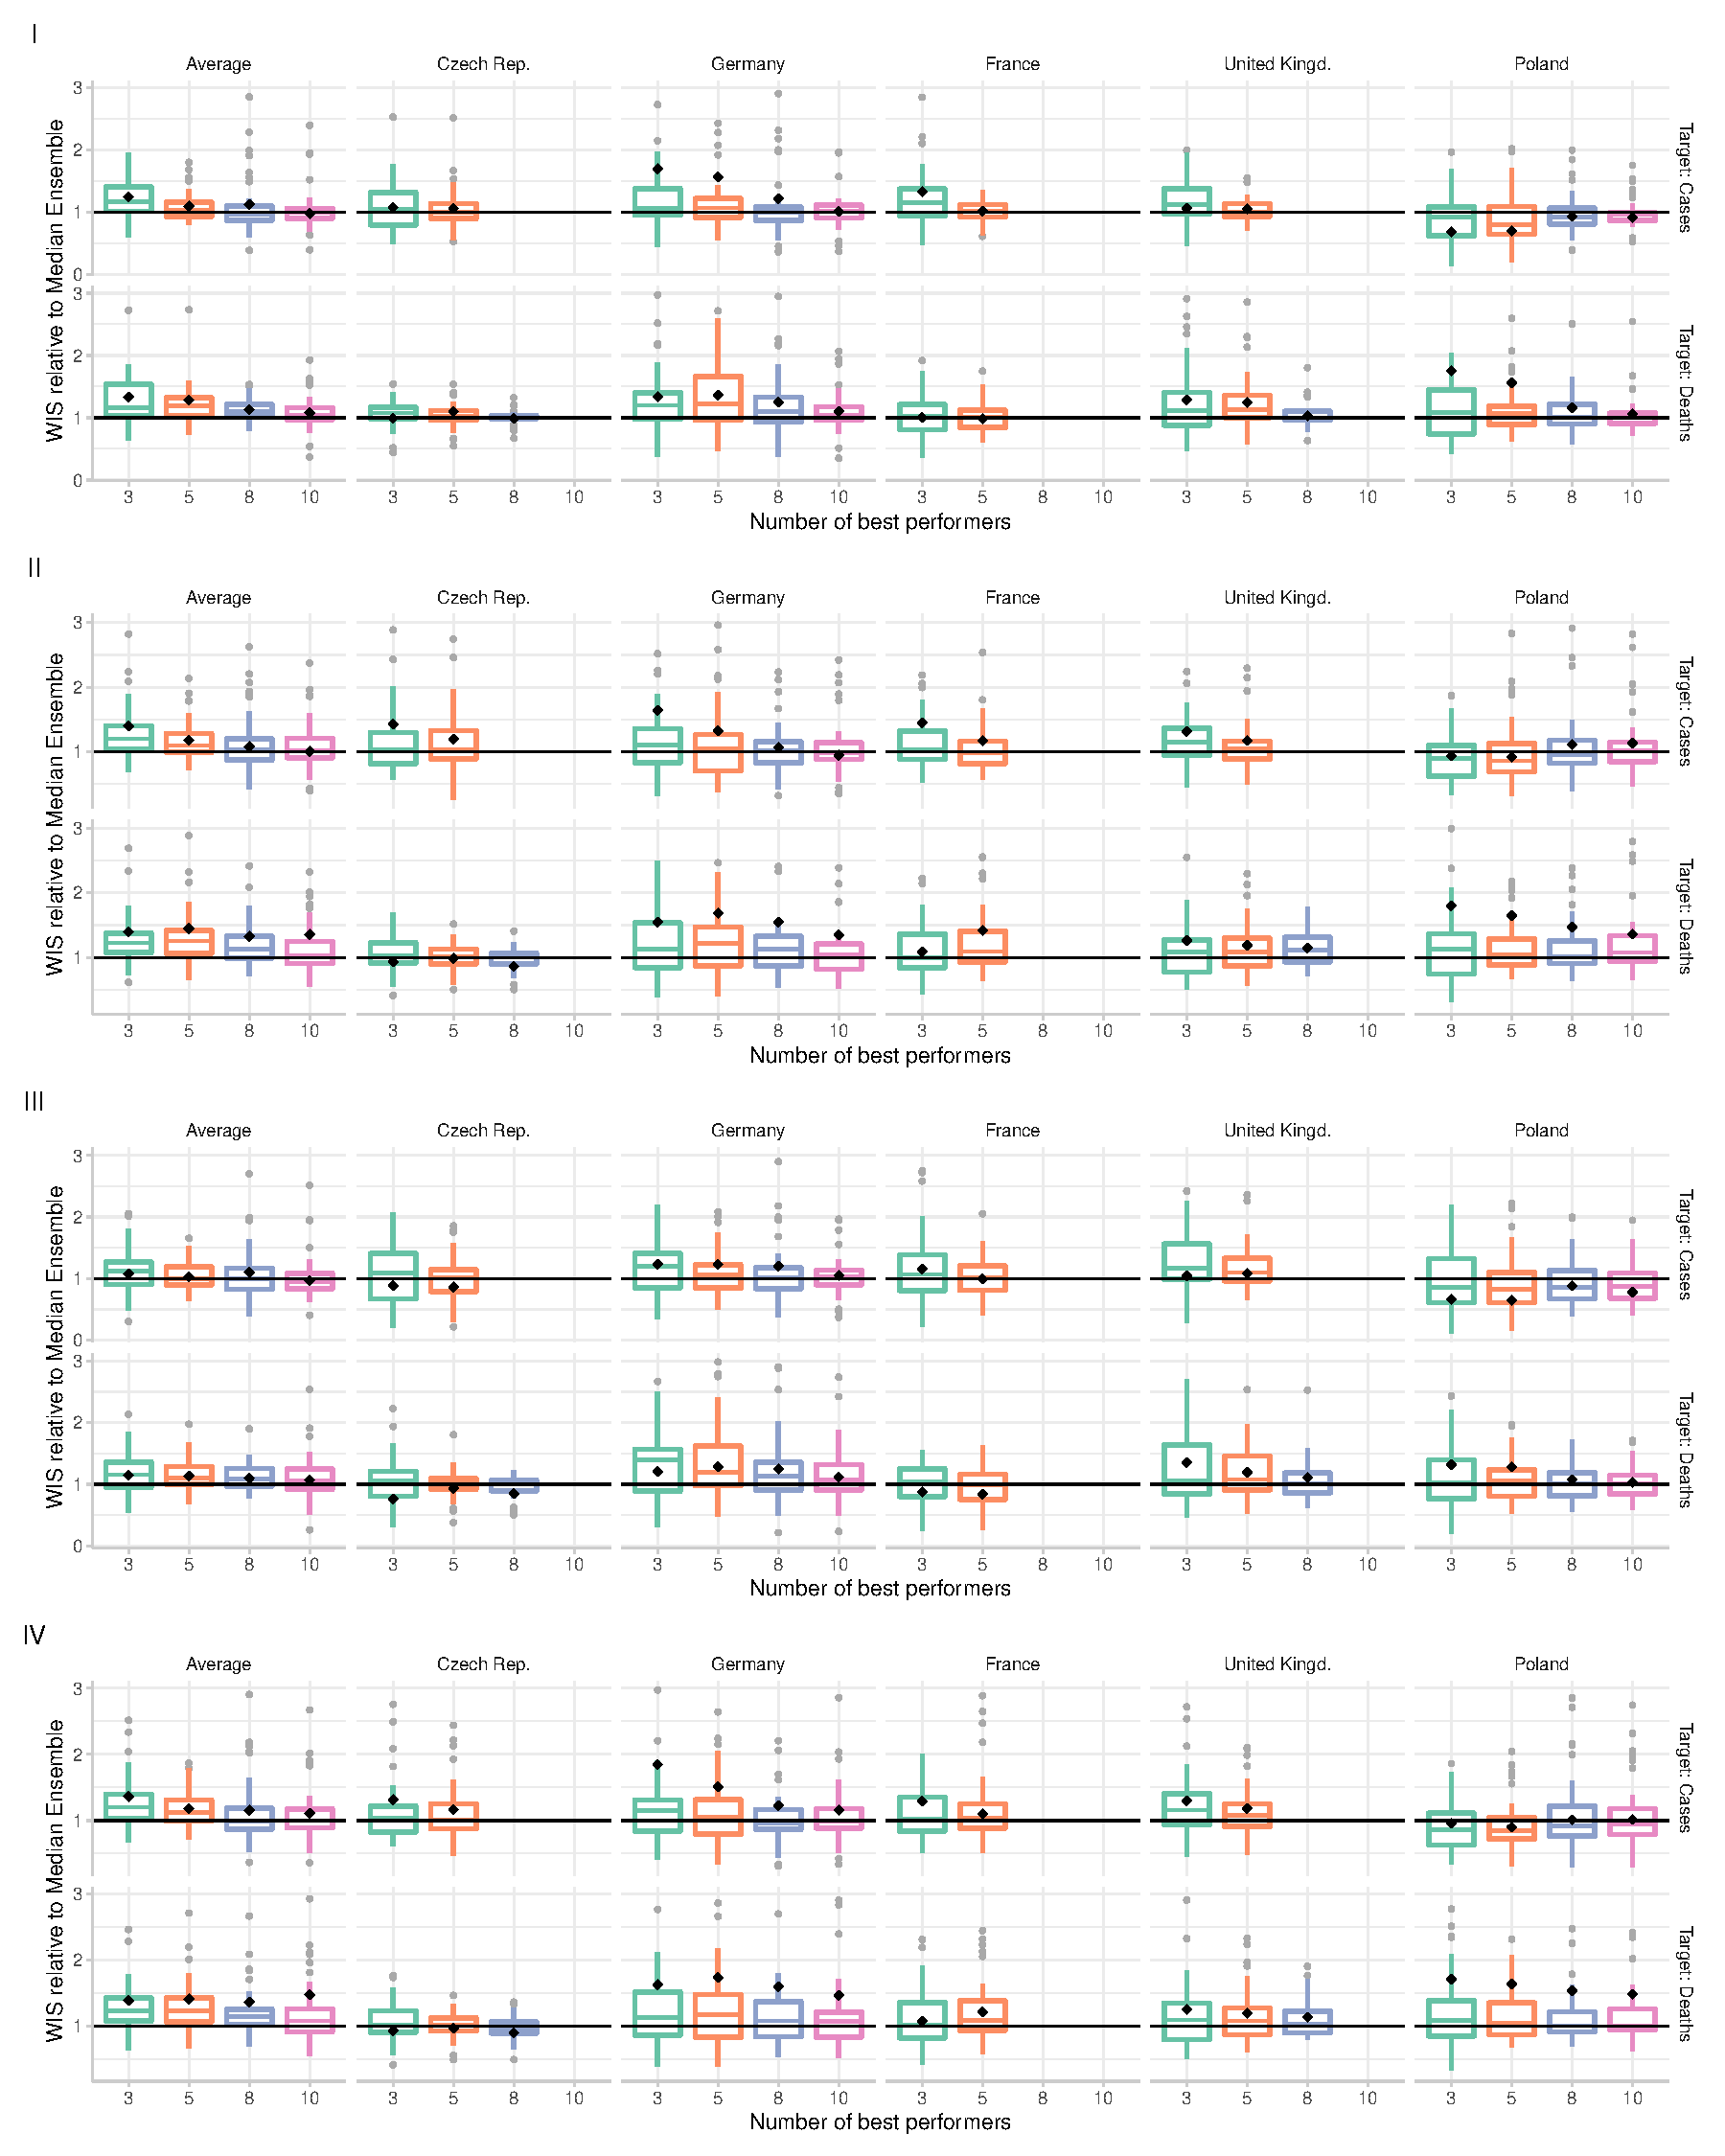
\includegraphics[width = 0.95\textwidth]{../plots/best_performers_boxplot}
\caption{\footnotesize{Boxplots showing the spread of the WIS of the selection ensemble methods (based on recent component forecast performance) relative to the benchmark (equally weighted median ensemble including all models), by location and number of best recent performers ($k$) included. The four panels show the resulting spreads when subsequently applying different ensemble methods to the selected component forecasts: The first panel (I) shows the results for the equally weighted median, the second panel (II) for the equally weighted mean, the third panel (III) for the inverse score weighted median and the fourth panel (IV) for the inverse score weighted mean. For all methods, selection of component forecasters and (if applicable) estimation of weights is based on performance in the past four weeks. Outliers with relative scores over 3 were excluded from the plots for legibility - to compensate for this, the diamond-shaped black points represent the mean relative score value. Values below one mean that the respective method outperforming the benchmark for the given target. Missing boxplots for a given $k$ correspond to the cases where the respective combination of location and target type did not have a sufficient model base to support the analysis.}}
\label{ref:best_perform_boxplot}
\end{figure}\\
We varied the number of component forecasts included, namely, we tried $k = 3,5,8,10$. For a given $k$, we excluded a location and target type combination if the size of its model base was smaller than $(k+2)$ for at least half of the study period, as as we believed that in these cases the analysis would conceptionally be too similar to an ensemble of all models (that is, there is no meaningful choice of ``best'' performers if almost all models are included over most of the study period) and could therefore portray the method more favorably than it is in actuality. Along the same lines, we considered accounting for the fact that the model base was generally smaller during the winter months, where the approach in principle was accordingly more similar to the benchmark. We however saw no meaningful differences in the results across different periods, so we report the results aggregated over the entire study period.\\
\begin{table}[t]
\centering
\begin{tabular}{lll}
\hline
location & target\_type & models\\
\hline
CZ & Cases & ILM-EKF (35), IEM\_Health-CovidProject (31), MUNI\_DMS-SEIAR (28)\\[0.1em]
DE & Cases & itwm-dSEIR (25), ILM-EKF (20), ITWW-county\_repro (16)\\[0.1em]
FR & Cases & ILM-EKF (34), USC-SIkJalpha (32), IEM\_Health-CovidProject (31)\\[0.1em]
GB & Cases & IEM\_Health-CovidProject (34), MUNI-ARIMA (27), ILM-EKF (23)\\[0.1em]
PL & Cases & MOCOS-agent1 (29), epiforecasts-EpiNow2 (23), ILM-EKF (21)\\[0.8em]
CZ & Deaths & UMass-MechBayes (36), ILM-EKF (28), epiforecasts-EpiNow2 (24)\\[0.1em]
DE & Deaths & HZI-AgeExtendedSEIR (28), RobertWalraven-ESG (18), USC-SIkJalpha (18)\\[0.1em]
FR & Deaths & RobertWalraven-ESG (32), UMass-MechBayes (32),\\
& & IEM\_Health-CovidProject (31), ILM-EKF (31)\\[0.1em]
GB & Deaths & IEM\_Health-CovidProject (26), USC-SIkJalpha (26), LANL-GrowthRate (21), \\
& & RobertWalraven-ESG (21), UMass-MechBayes (21)\\[0.1em]
PL & Deaths & MOCOS-agent1 (37), UMass-MechBayes (29), ILM-EKF (27)\\
\hline
\end{tabular}
\caption{Table showing models chosen}
\label{tab:bp_chosenmods}
\end{table}
Before we turn to the results in performance, we want to shortly pull attention to Table \ref{tab:bp_chosenmods}, which, for $k = 5$, displays each location's top three chosen models using the method, separately for Cases and Deaths. We do observe that there are some models (most prominently \texttt{ILM-EKF} for Cases and \texttt{UMass-MechBayes} for Deaths) that are chosen across most or all locations. However, we also both see models (such as \texttt{epiforecasts-EpiNow2} or \texttt{MUNI-ARIMA}) that in principle submit forecasts for all locations, but are more often chosen at some locations than others, as well as some models, such as \texttt{ITWW-county-repro} or \texttt{MOCOS-agent1} that forecast for only one or two locations. Recall that we argued that the U.S. approach could be fundamentally flawed for an application in the European Hub as it does not account for the fact that models could have considerable variations in performance across locations. While it does seem to prove true that there are considerable performance differences across locations and a more flexible method will accordingly choose different models, as we will shortly see, accounting for this is not enough to gain competitive performance in the European Hub.\medskip\\
% As we will shortly see, but we thereby argue that we have ruled out the lack in flexibility in model choosing induced by the aforementioned U.S. approach as the sole cause of the fact that the method does not work all too well in the European Hub. Thus, even though we, contrary to the U.S. Hub approach, addressed both the lack in flexibility and the number of models , thereby ruling these out as the sole causes of the issue.\\
%- this is just to demonstrate that the reason for bad performance is not only due to the inflexibility in model selection.\\
%a. we see that e.g. mocosagent would have reduced the ensemble size.
%b. \\
\begin{table}[t]
\centering
\begin{tabular}{lrlrrrrrr}
\hline
model & nmod & target\_type & Average & CZ & DE & FR & GB & PL\\
\hline
unw. median & 5 & Cases & 1.10 & 1.06 & 1.57 & 1.02 & 1.05 & 0.70\\
weighted median & 5 & Cases & 1.03 & 0.87 & 1.23 & 0.99 & 1.09 & 0.65\\[0.4em]
unw. mean & 5 & Cases & 1.18 & 1.20 & 1.33 & 1.17 & 1.18 & 0.92\\
weighted mean & 5 & Cases & 1.18 & 1.17 & 1.51 & 1.10 & 1.18 & 0.90\\[0.4em]
unw. median & 10 & Cases & 0.98 & - & 1.01 & - & - & 0.91\\
weighted median & 10 & Cases & 0.97 & - & 1.05 & - & - & 0.78\\[0.4em]
unw. mean & 10 & Cases & 1.01 & - & 0.95 & - & - & 1.14\\
weighted mean & 10 & Cases & 1.11 & - & 1.16 & - & - & 1.02\\[0.4em]
unw. median & 5 & Deaths & 1.29 & 1.10 & 1.36 & 0.98 & 1.24 & 1.56\\
weighted median & 5 & Deaths & 1.13 & 0.93 & 1.29 & 0.84 & 1.19 & 1.28\\[0.4em]
unw. mean & 5 & Deaths & 1.45 & 0.99 & 1.68 & 1.42 & 1.19 & 1.65\\
weighted mean & 5 & Deaths & 1.41 & 0.97 & 1.73 & 1.21 & 1.19 & 1.63\\[0.4em]
unw. median & 10 & Deaths & 1.08 & - & 1.10 & - & - & 1.06\\
weighted median & 10 & Deaths & 1.07 & - & 1.12 & - & - & 1.03\\[0.4em]
unw. mean & 10 & Deaths & 1.36 & - & 1.35 & - & - & 1.36\\
weighted mean & 10 & Deaths & 1.47 & - & 1.46 & - & - & 1.48\\
\hline
\end{tabular}
\caption{Blabla}
\label{tab:rel_wis_best_performers}
\end{table}
We now turn to an actual discussion of the results. The aggregated results can be seen in Table \ref{tab:rel_wis_best_performers}, which shows the ratio of the average WIS obtained by the respective method and that of the equally weighted median ensemble including all available models. We furthermore show the variation of relative WIS obtained at each target, separately by location and the two series, in the boxplots in Figure \ref{ref:best_perform_boxplot}. For both, we additionally included the relative scores that result from averaging across all locations.\\
For the ``average location'', we can directly see that for all numbers of component forecasters included in the best performers set, scores are consistently either similar to or worse than for the equally weighted median ensemble including all models. Choosing a subset of best performers thus does not seem to be a viable alternative to the benchmark, whether or not the models are subsequently weighted. Nevertheless, we want to discuss some interesting trends and results, as well as attempt to establish reasons/heuristics for why the approach might fail.\\
As a general trend, all approaches tend to work better the more models are included: Figure \ref{ref:best_perform_boxplot} shows that variability in performance mostly decreases and the median and average relative scores move closer to one with increasing $k$. This suggests that the positive effect of ensemble size outweighs that of selecting models - the big exception here is the cases series for Poland, which we will discuss separately further down. In other words, the closer the setting is to an ensemble that indiscriminately includes all component models, the better, whether or not the models are subsequently weighted. However, we again make not of the fact that our model base is very small. It could be the case that there exists a critical threshold of number of models, after which the added marginal benefit of adding another model is smaller and benefits from model selection can actually be realized. If this were the case, we could simply still be sitting firmly in the region of ``more models are always better''.\\
%We thus expect that it is likely the case that one either needs  there exists a critical threshold for ensemble size that one needs to clear before selection makes sense, as this will give a larger pool of models to choose from. \\ in lieu of the existence of some actual top performers. It could thus be that for the locations (with the exception of some actual top performers) are still in a range of "more models are always better"\\
Furthermore, we see that the mean approaches, whether weighted or not, generally see a higher average relative score, again highlighting the general vulnerability of the mean ensemble to outlying forecasts and thereby the benefit of using the more robust median ensemble, especially when working with a small number of component forecasts. 
%furthermore supporting the claim that the mean ensemble can undesirably produce outlying forecasts and is not as robust, especially when model base is small
Moreover, while additional weighting seems to either not impact or improve the median ensemble, it sometimes has large negative effect on the average score of the mean ensemble, for instance for the Case series in Germany for $k = 5$ - from the boxplots, it becomes clear that this mostly stems from large outlying relative scores. This is likely due to the fact that the mean ensemble is already more vulnerable to deteriorations in performance from one of its member forecasts, especially in small model sets - if such a forecast is additionally given a higher weight due to previous good performance, we can expect performance to further decline in such a situation.\\
Thus, since both the weighted and unweighted mean compared unfavorably, we generally focus our remaining discussion on the respective median approaches. \medskip\\
The only case where we see a slight improvement of scores for the average location relative to the benchmark is for forecasting Cases and $k = 10$ - the individual results however show that this is only due to the results from Poland, where performance is actually improved across all $k$, especially for the weighted median ensemble. We now want to investigate why this is the case, exemplary for $k = 10$ and in contrast to the Cases series from Germany. Afterwards, we also turn to a short discussion about forecasting Deaths.\\
Thus, consider Figures \ref{fig:bpweights_de} and \ref{fig:bpweights_pl}, where we display the weights given over time to the five models chosen most often, as well as those models' relative WIS, their 2-week ahead predictions and the WIS of the weighted median relative to the benchmark, for Poland and Germany, respectively.
\begin{figure}
\centering
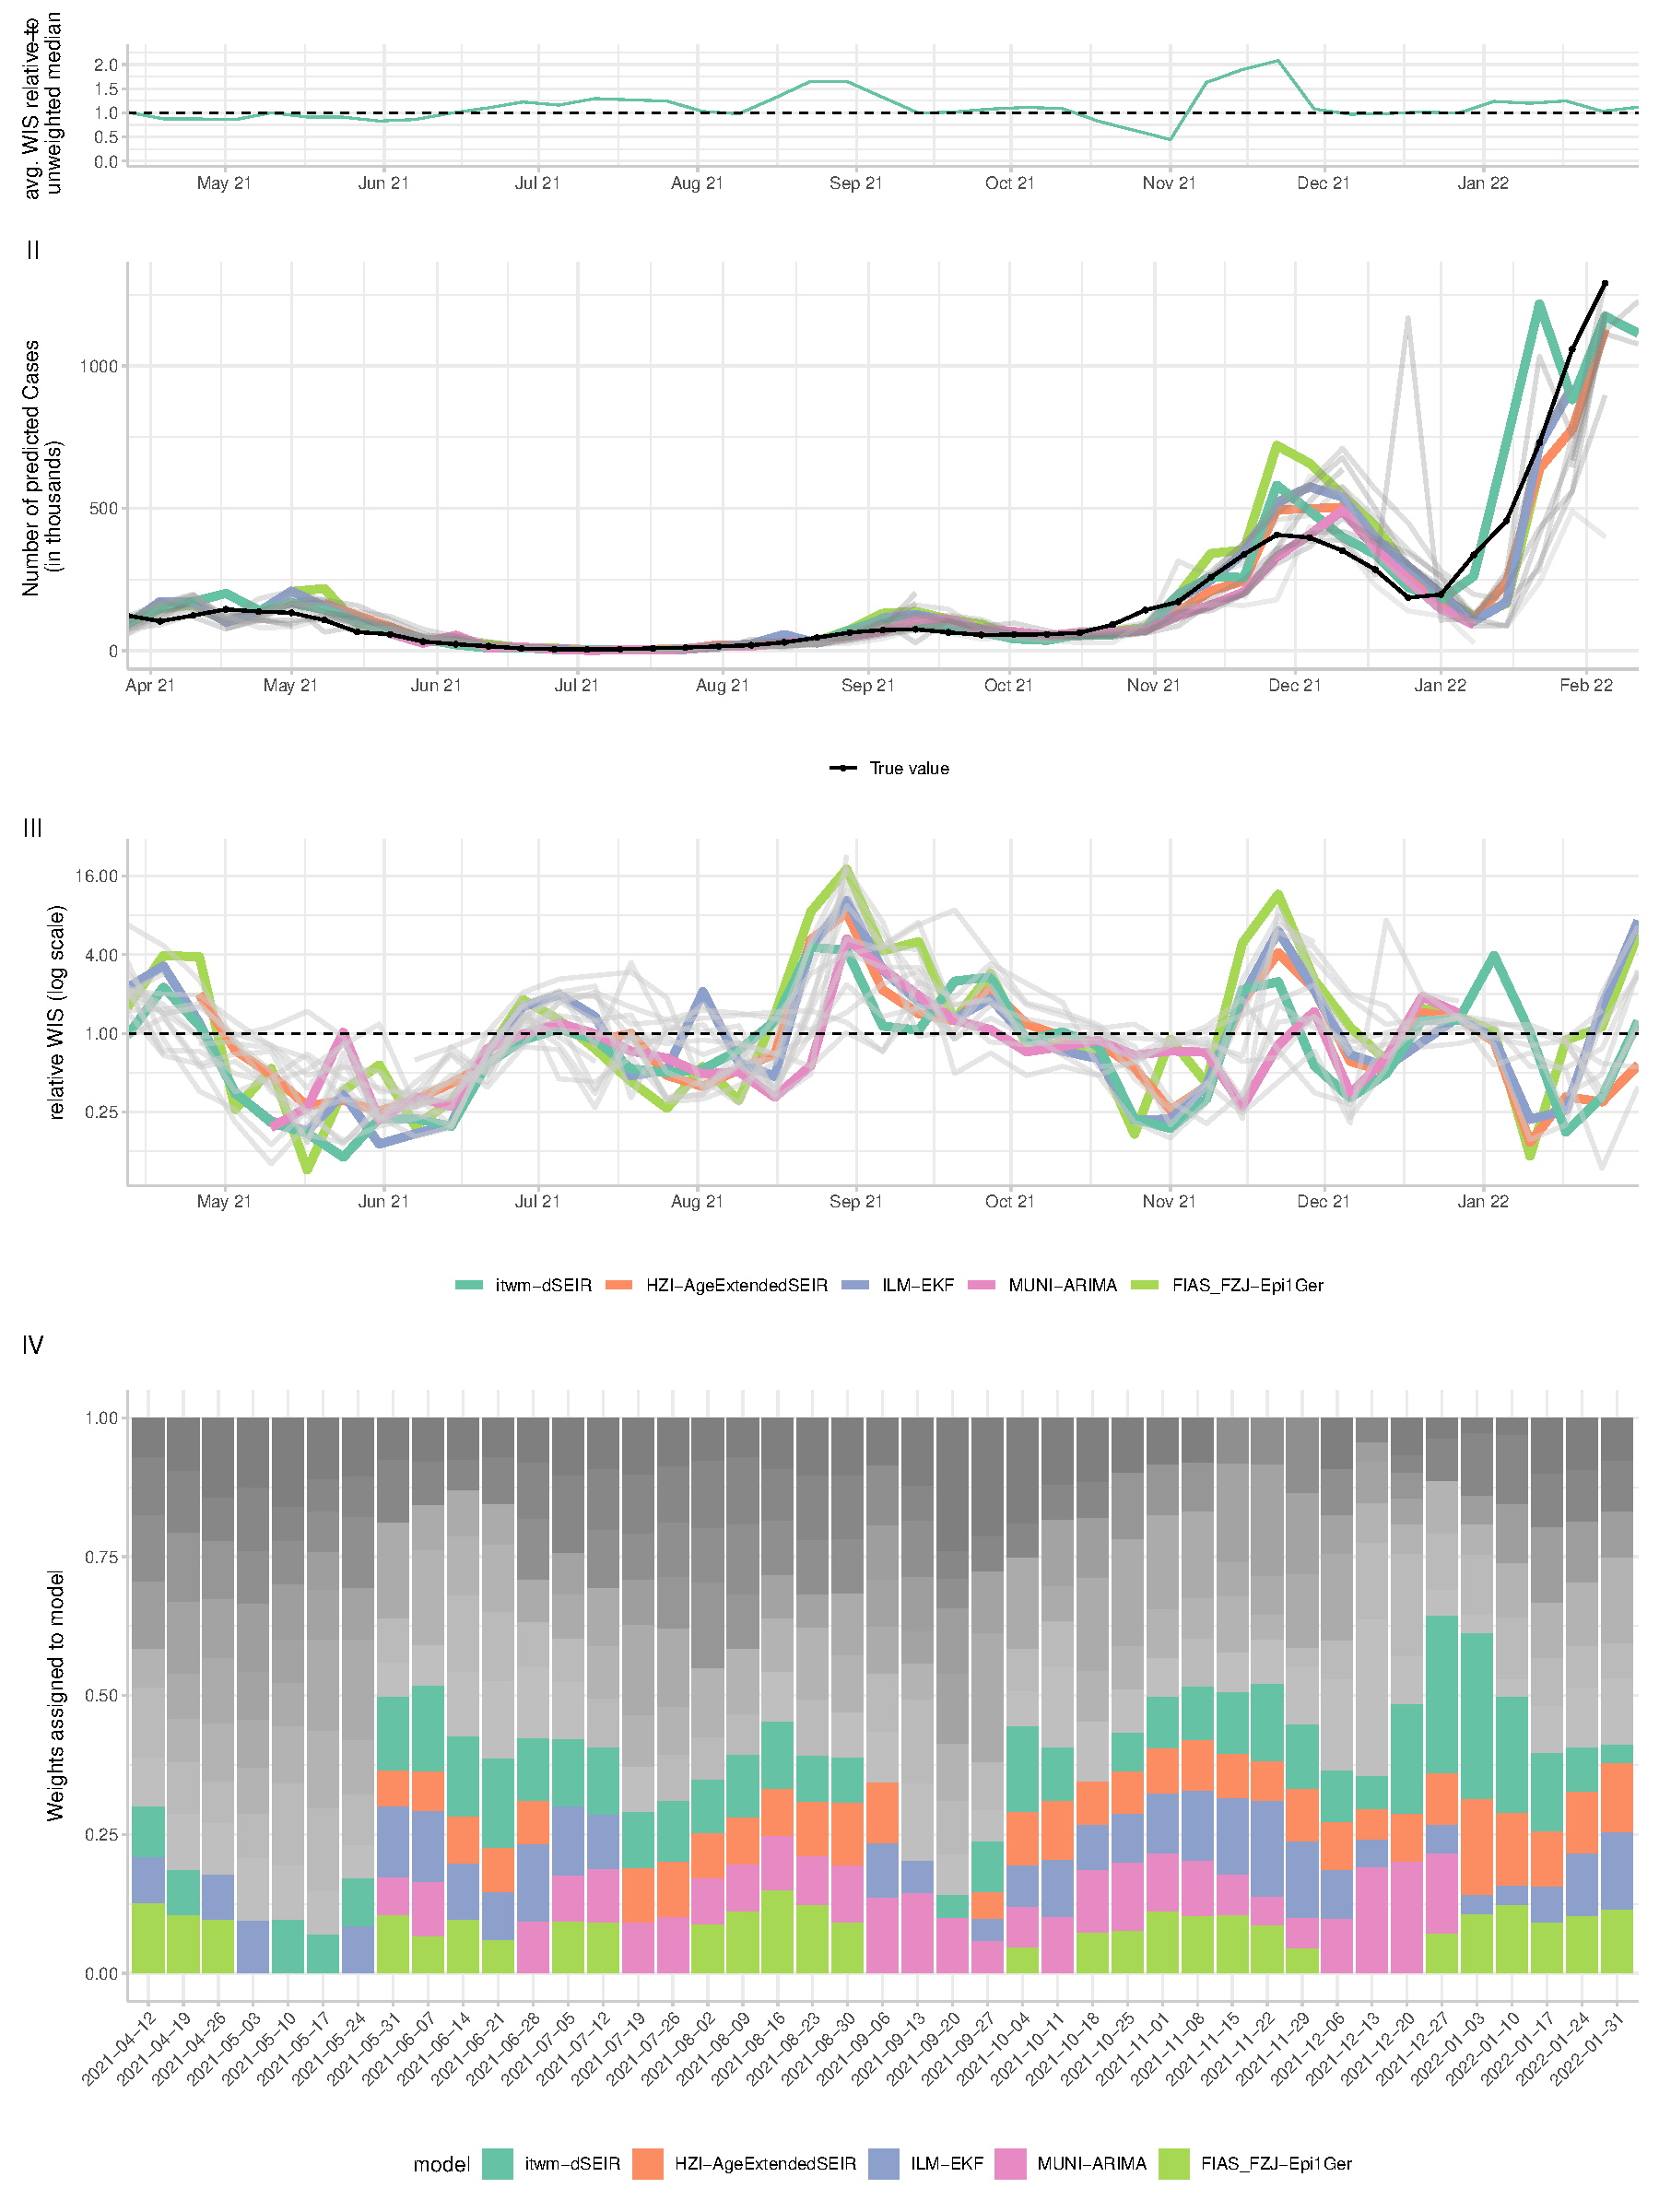
\includegraphics[width = 0.9\textwidth]{../plots/best_performers_weights_de}
\caption{\footnotesize{Performance of weekly case forecasts for Germany, for the weighted median selection ensemble based on the ten component forecast with best performance, and its component forecasts. Component forecasts are selected and weighted based on their performance in the most recent four weeks. Across all plots, the five models chosen most often for the selection ensemble are highlighted. Panel (I) shows the relative performance of the weighted median selection ensemble based on recent component forecast performance, relative to the benchmark (unweighted median ensemble including all models). Panel (II) shows two week ahead predictions of all component forecasts, as well as the observed values of the series. Panel (III) shows performance of component forecasts over time, in terms of relative WIS. Panel (IV) shows the weekly distribution of weights given to component forecasts. Note that as forecasts are scored by the forecast date, performance measure series lead ahead of the observed incidence series. Plot inspired by \cite{ray_comparing_2022}.}}
\label{fig:bpweights_de}
\end{figure}\\
Figure \ref{fig:bpweights_de} for Germany shows the fundamental issue of selecting and/or weighting models based on recent performance, which is the potential non-stationarity of model's relative performance and the thereby induced unreliability of using past performance as a predictor for current performance. We will now walk the reader through these plots to illustrate that issue.\footnote{At this point, we want to again explicitly mention an important characteristic of the way forecasts are scored here, to clarify the way these plots need to be interpreted. We score models by the forecast date, not by the target date. That is, if a model issues a 3-week forecast on May 3 that severely overshoots the target as it realized on May 22, this will be reflected on its score on May 3. Thus, if models for instance overshoot at longer horizons, this is reflected in the scores \textit{before} the target date.} Throughout the summer months of 2021, the weighted method performed comparatively to the benchmark, as it could identify component forecasts that - to a certain extent - had consistent good performance relative to other forecasters. As autumn approaches, it has placed close to half of its weight on four of these component forecasts. It is at this time that cases start rising and (especially at longer horizons), these models overshoot the target. Critically, they overshoot the target more than alternative models: while other models mostly exhibit similar behavior and thus also compare unfavorably to the baseline model of ``no change'', they still stay closer to the target and the ensemble would thus have fared better if it had drawn from its entire model base and not placed undue weight on a small number of component forecasts - as a consequence, the benchmark (which includes all models) performs better than the weighted method during this time.\\ 
Thereafter, during the month of September, these models are sequentially dropped from the set of best performers and hence given zero weight, but only after they have influenced and thus worsened the performance of the ensemble. Moreover, we can see the same behavior again during December of 2021, where models that have received higher weight subsequently overshoot the target and hence undermine the ensemble's performance - the most notable example in this regard is perhaps \texttt{FIAS\_FZJ-Epi1Ger}, which receives especially high relative WIS during these moments of ``collective overshooting'' and is consequentially most often dropped altogether from the selected ensemble.\\ 
Thus, while the method stays somewhat close to benchmark performance when averaging over all forecast dates (at a relative score of 1.05), we can see that it undesirably fails in critical times, making it altogether an unattractive alternative to the benchmark.\medskip\\
%Consider, for instance, the model \texttt{FIASFZJ-Epi1Ger} - throughout the summer months of 2021, it performs relatively well and is awarded positive weight in the ensemble.  during the late fall period of 2021 it issues fjust as its performance recovers during the fall and it is again given positive weight, its performance deteriorates again.\\
\begin{figure}
\centering
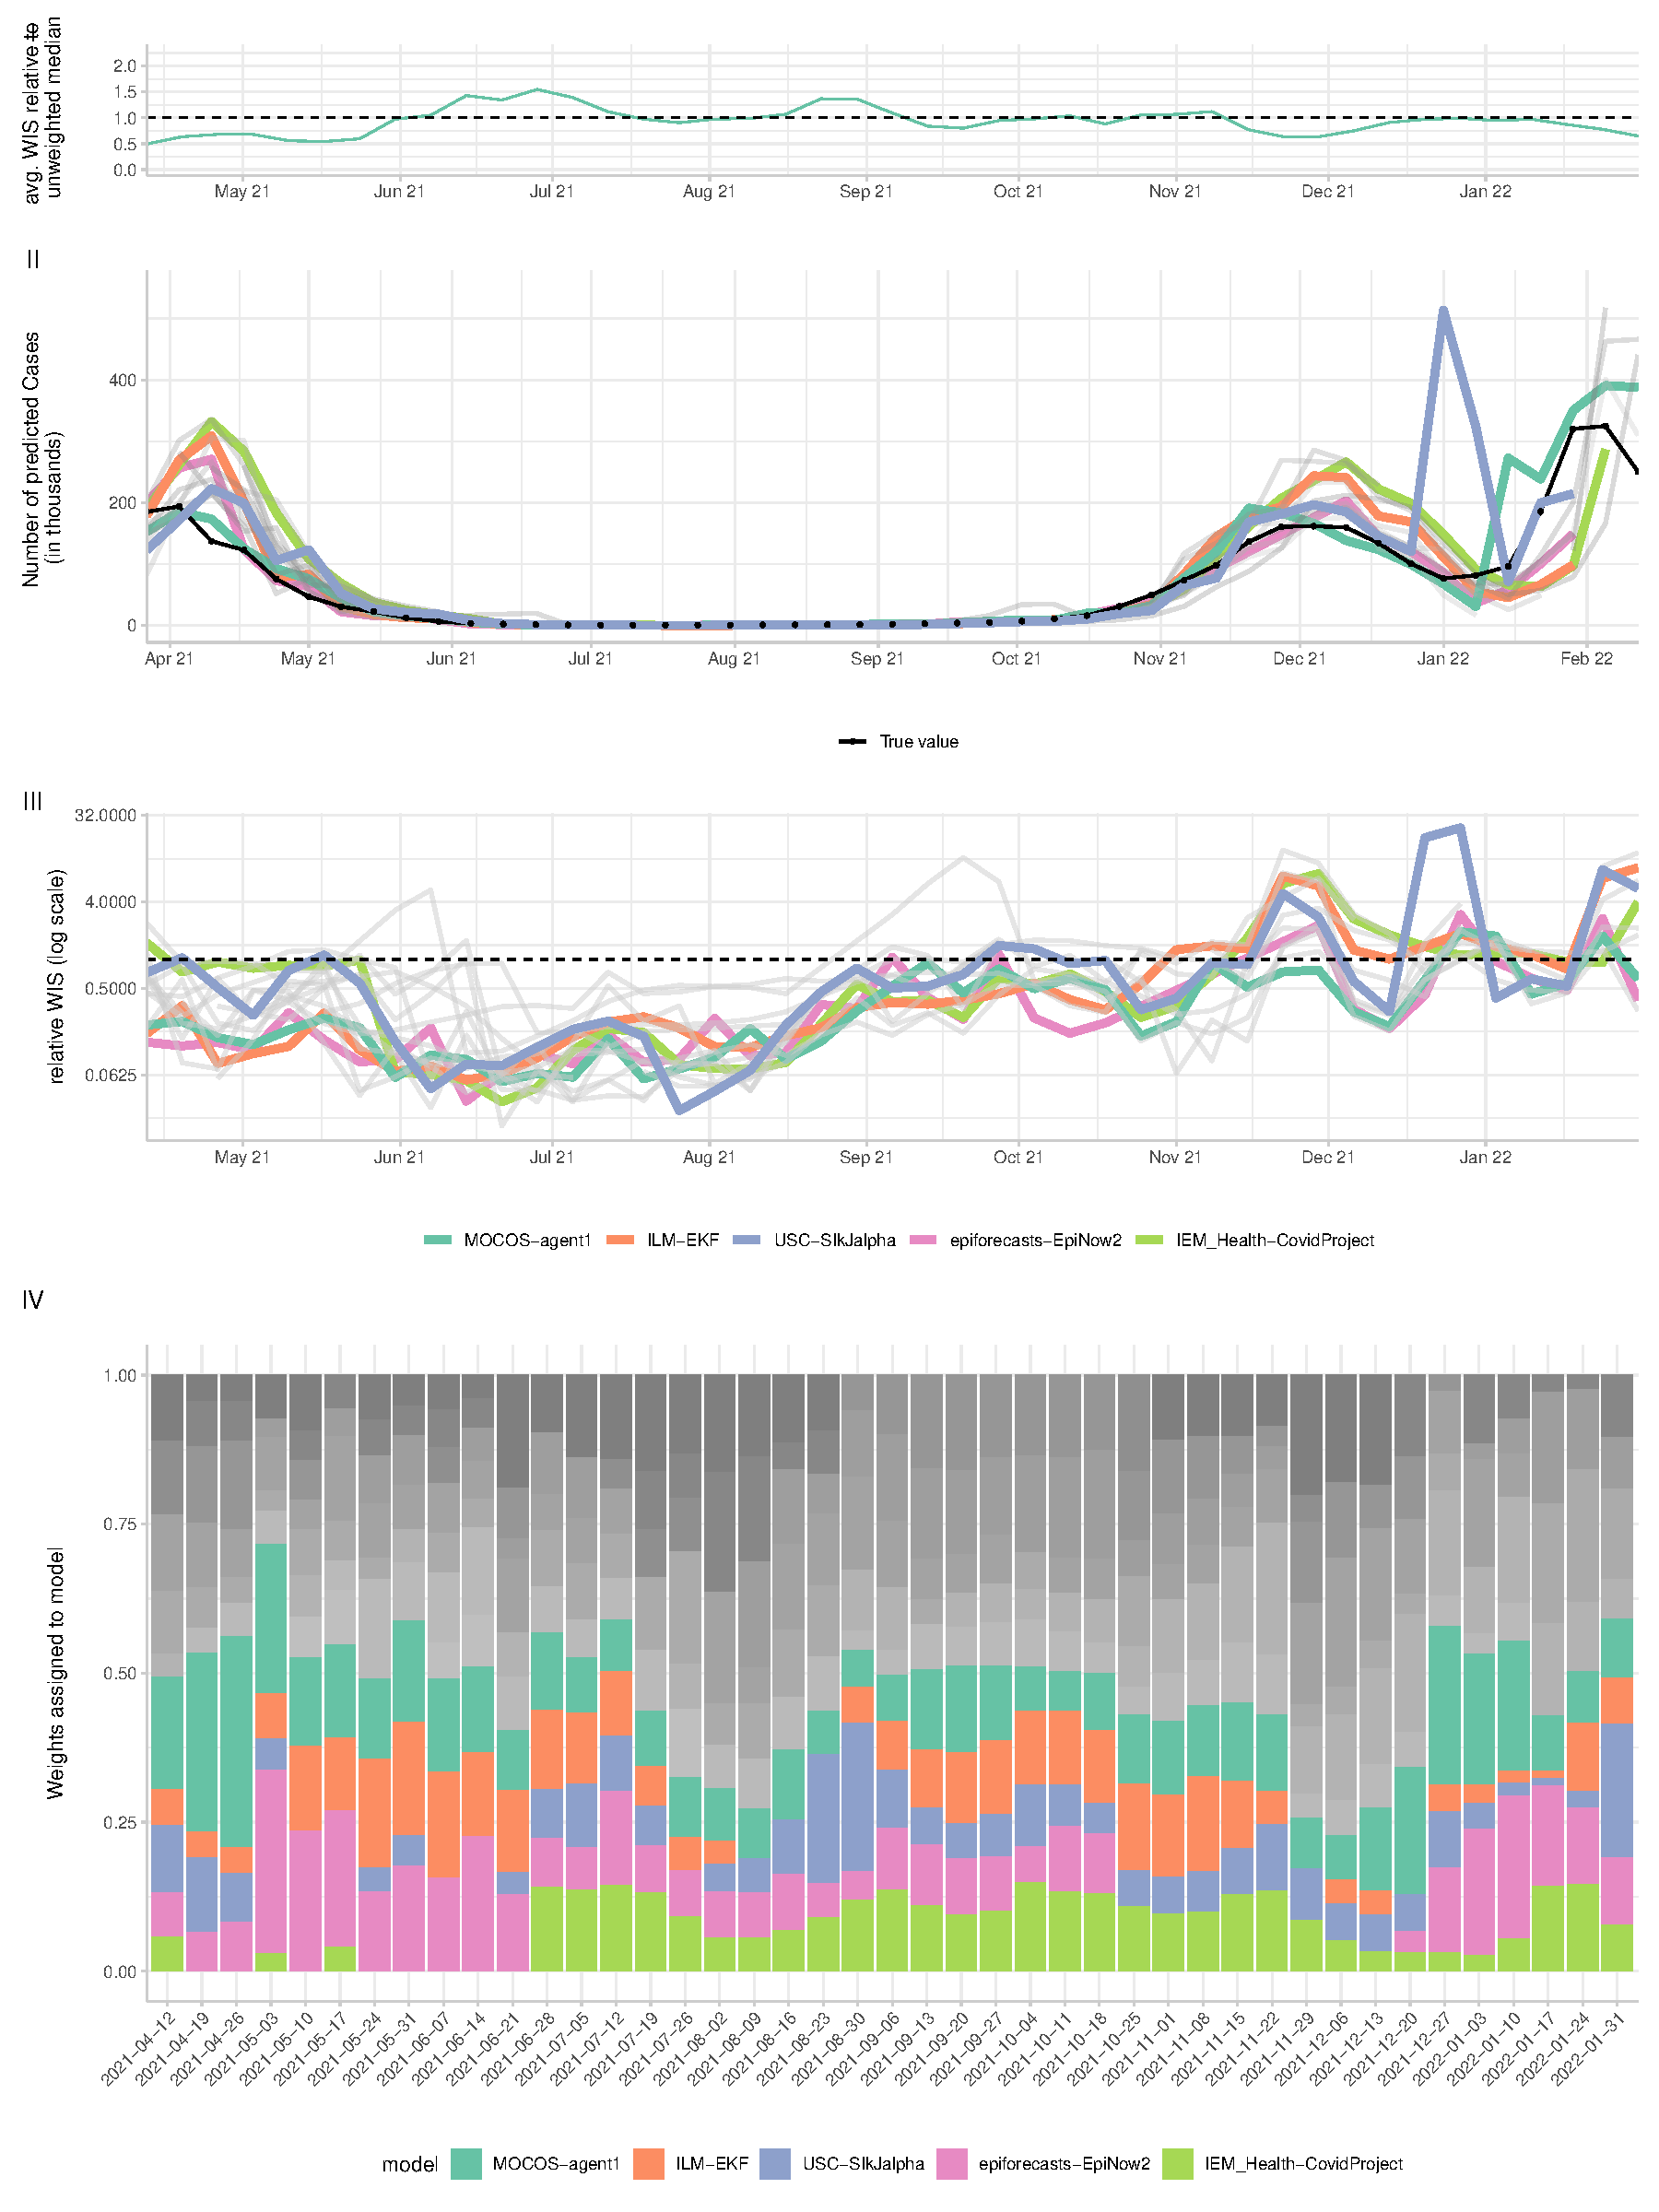
\includegraphics[width = 0.9\textwidth]{../plots/best_performers_weights_pl}
\caption{\footnotesize{Performance of weekly case forecasts for Poland, for the weighted median selection ensemble based on the ten component forecast with best performance, and its component forecasts. Component forecasts are selected and weighted based on their performance in the most recent four weeks. Across all plots, the five models chosen most often for the selection ensemble are highlighted. Panel (I) shows the relative performance of the weighted median selection ensemble based on recent component forecast performance, relative to the benchmark (unweighted median ensemble including all models). Panel (II) shows two week ahead predictions of all component forecasts, as well as the observed values of the series. Panel (III) shows performance of component forecasts over time, in terms of relative WIS. Panel (IV) shows the weekly distribution of weights given to component forecasts. Note that as forecasts are scored by the forecast date, performance measure series lead ahead of the observed incidence series. Furthermore, note that the y-axis of panel (I) was deliberately stretched for compatibility with panel (I) in Figure \ref{fig:bpweights_de}. Plot inspired by \cite{ray_comparing_2022}.}}
\label{fig:bpweights_pl}
\end{figure}
In contrast to this, we now discuss the Case series for Poland, where, as mentioned, the weighted selection ensemble performs substantially better in the aggregate. At the beginning of the study period, the selection ensemble places a large proportion of its total weight on three performers (\texttt{MOCOS-agent1}, \texttt{ILM-EKF} and \texttt{epiforecasts-EpiNow2}) that perform relatively well at predicting the decline in case numbers. As a consequence, the weighted selection ensemble compares quite favorably to the benchmark. Subsequently, during the summer and fall months, model performance is overall more similar and relative performance stays mostly close to one - \todos{find out why it performs a little worse at times }% we would argue that the selection method mostly performs a little worse here compared to the benchmark due to the fact that it effectively excludes a large number of models. 
But perhaps most importantly, heading into the winter months of 2021, where Poland (similar to Germany and some other countries in the set) experiences a sharp rise in cases followed by a decline and subsequently another sharp rise, it manages to more heavily weight some models that exhibit relatively less overshooting behavior, thereby overall performing better than the benchmark. \\We would also argue that the behavior near these critical times is actually more meaningful than that during the summer months which overall have very low incidence rates and are thus not of the same level of interest to decision makers. To conclude the discussion for Poland, we would thus argue that Poland contains models (most notably the agent-based \texttt{MOCOS-agent1}, which only predicts in Poland) that seem to exhibit particular foresight when forecasting cases - it thus makes sense to more heavily rely on these models. \\%In lieu of the existence of these models, it doesn't really make sense.\\ 
However, there is of course no guarantee that this behavior could be replicated for the same series during other critical times. Furthermore, for the other countries in the set, we on the one hand also obtain a higher relative skill score in the aggregate compared to the benchmark and can observe similar trends to that exhibited by Germany. Thus, we argue that a central problem with the selection methods is that, as a model might exhibit good performance over a given time period and is thus given nonzero or higher weight in the ensemble, the selection ensemble increasingly makes itself vulnerable to performance fluctuations of such a model.\\ 
Specifically for the Cases series in the U.S. Hub, \cite{ray_comparing_2022} also state that they have observed similar behavior: they give the explanation that the best performing component models for forecasting Cases were generally those that were observed to extrapolate recent trends. This would mean that, as trends change from mostly level to increasing, these models would actually cease to be the ``best'' models, as extrapolating recent trends is fundamentally also associated with overshooting peaks. This is in and of itself an undesirable behavior, but in addition (due to the innately higher level of the series during a peak) also gives higher absolute scores to those forecasts as a consequence.\\
%the ``best'' forecasting models for Cases would also change from those . 
However, precisely as these changes in trends happens, the weighted selection ensemble has already selected for and placed more weight on models that performed well in recent weeks, thereby making itself more vulnerable to their behavior and excluding models which would have mitigated the trend-extrapolating (i.e., overshooting) behavior. By the time it has adapted to this and accordingly downweighted the overshooting models, the peak will have usually already passed. While we can't claim without fail that this is the sole and root cause of the issue, this explanation is most in line with what we have discussed and similar trends we observed for the other countries in the set.\medskip\\
Pertaining to the Deaths series, our results somewhat diverge from those in the U.S. Hub, where the series sees consistently improved performance from weighted selection. In our case, in the aggregate, weighted selection actually performs slightly worse for forecasting deaths than for forecasting cases, although we again must note that the somewhat diverging results across locations and therefore would hesitate to call the aggregate difference meaningful. Nevertheless, we can definitely not claim a consistent improvement as in the U.S. Hub.\\
As an exemplary illustration for the Deaths series, we now perform the same analysis for the United Kingdom and $k = 5$ in Figure \ref{fig:bpweights_gbdeaths}. In panel (III), we see that overall, most models seem to be similarly good at forecasting deaths - in fact, over- and under-prediction of the target (and thereby fluctuations in performance) seem to be happening at random (i.e., non-predictable) times, which leaves the ensemble usually starting to put weight on a component forecast right as its performance starts to deteriorate again. This is also reflected in the assigned weights, with models usually not staying in the set for prolonged periods. While we thus don't observe performance that is ever as detrimental as that which we described for Germany near peak times, the lack of consistent performance in any component forecasts and the thereby induced failure of the selection method to pick out forecasters at the precise times where they are actually performing well means that the weighted selection method accrues continually slightly higher scores over the entire study period. Thus, the weighted selection ensemble receives a bad score compared to the benchmark averaged over the entire period.\\
\begin{figure}
\centering
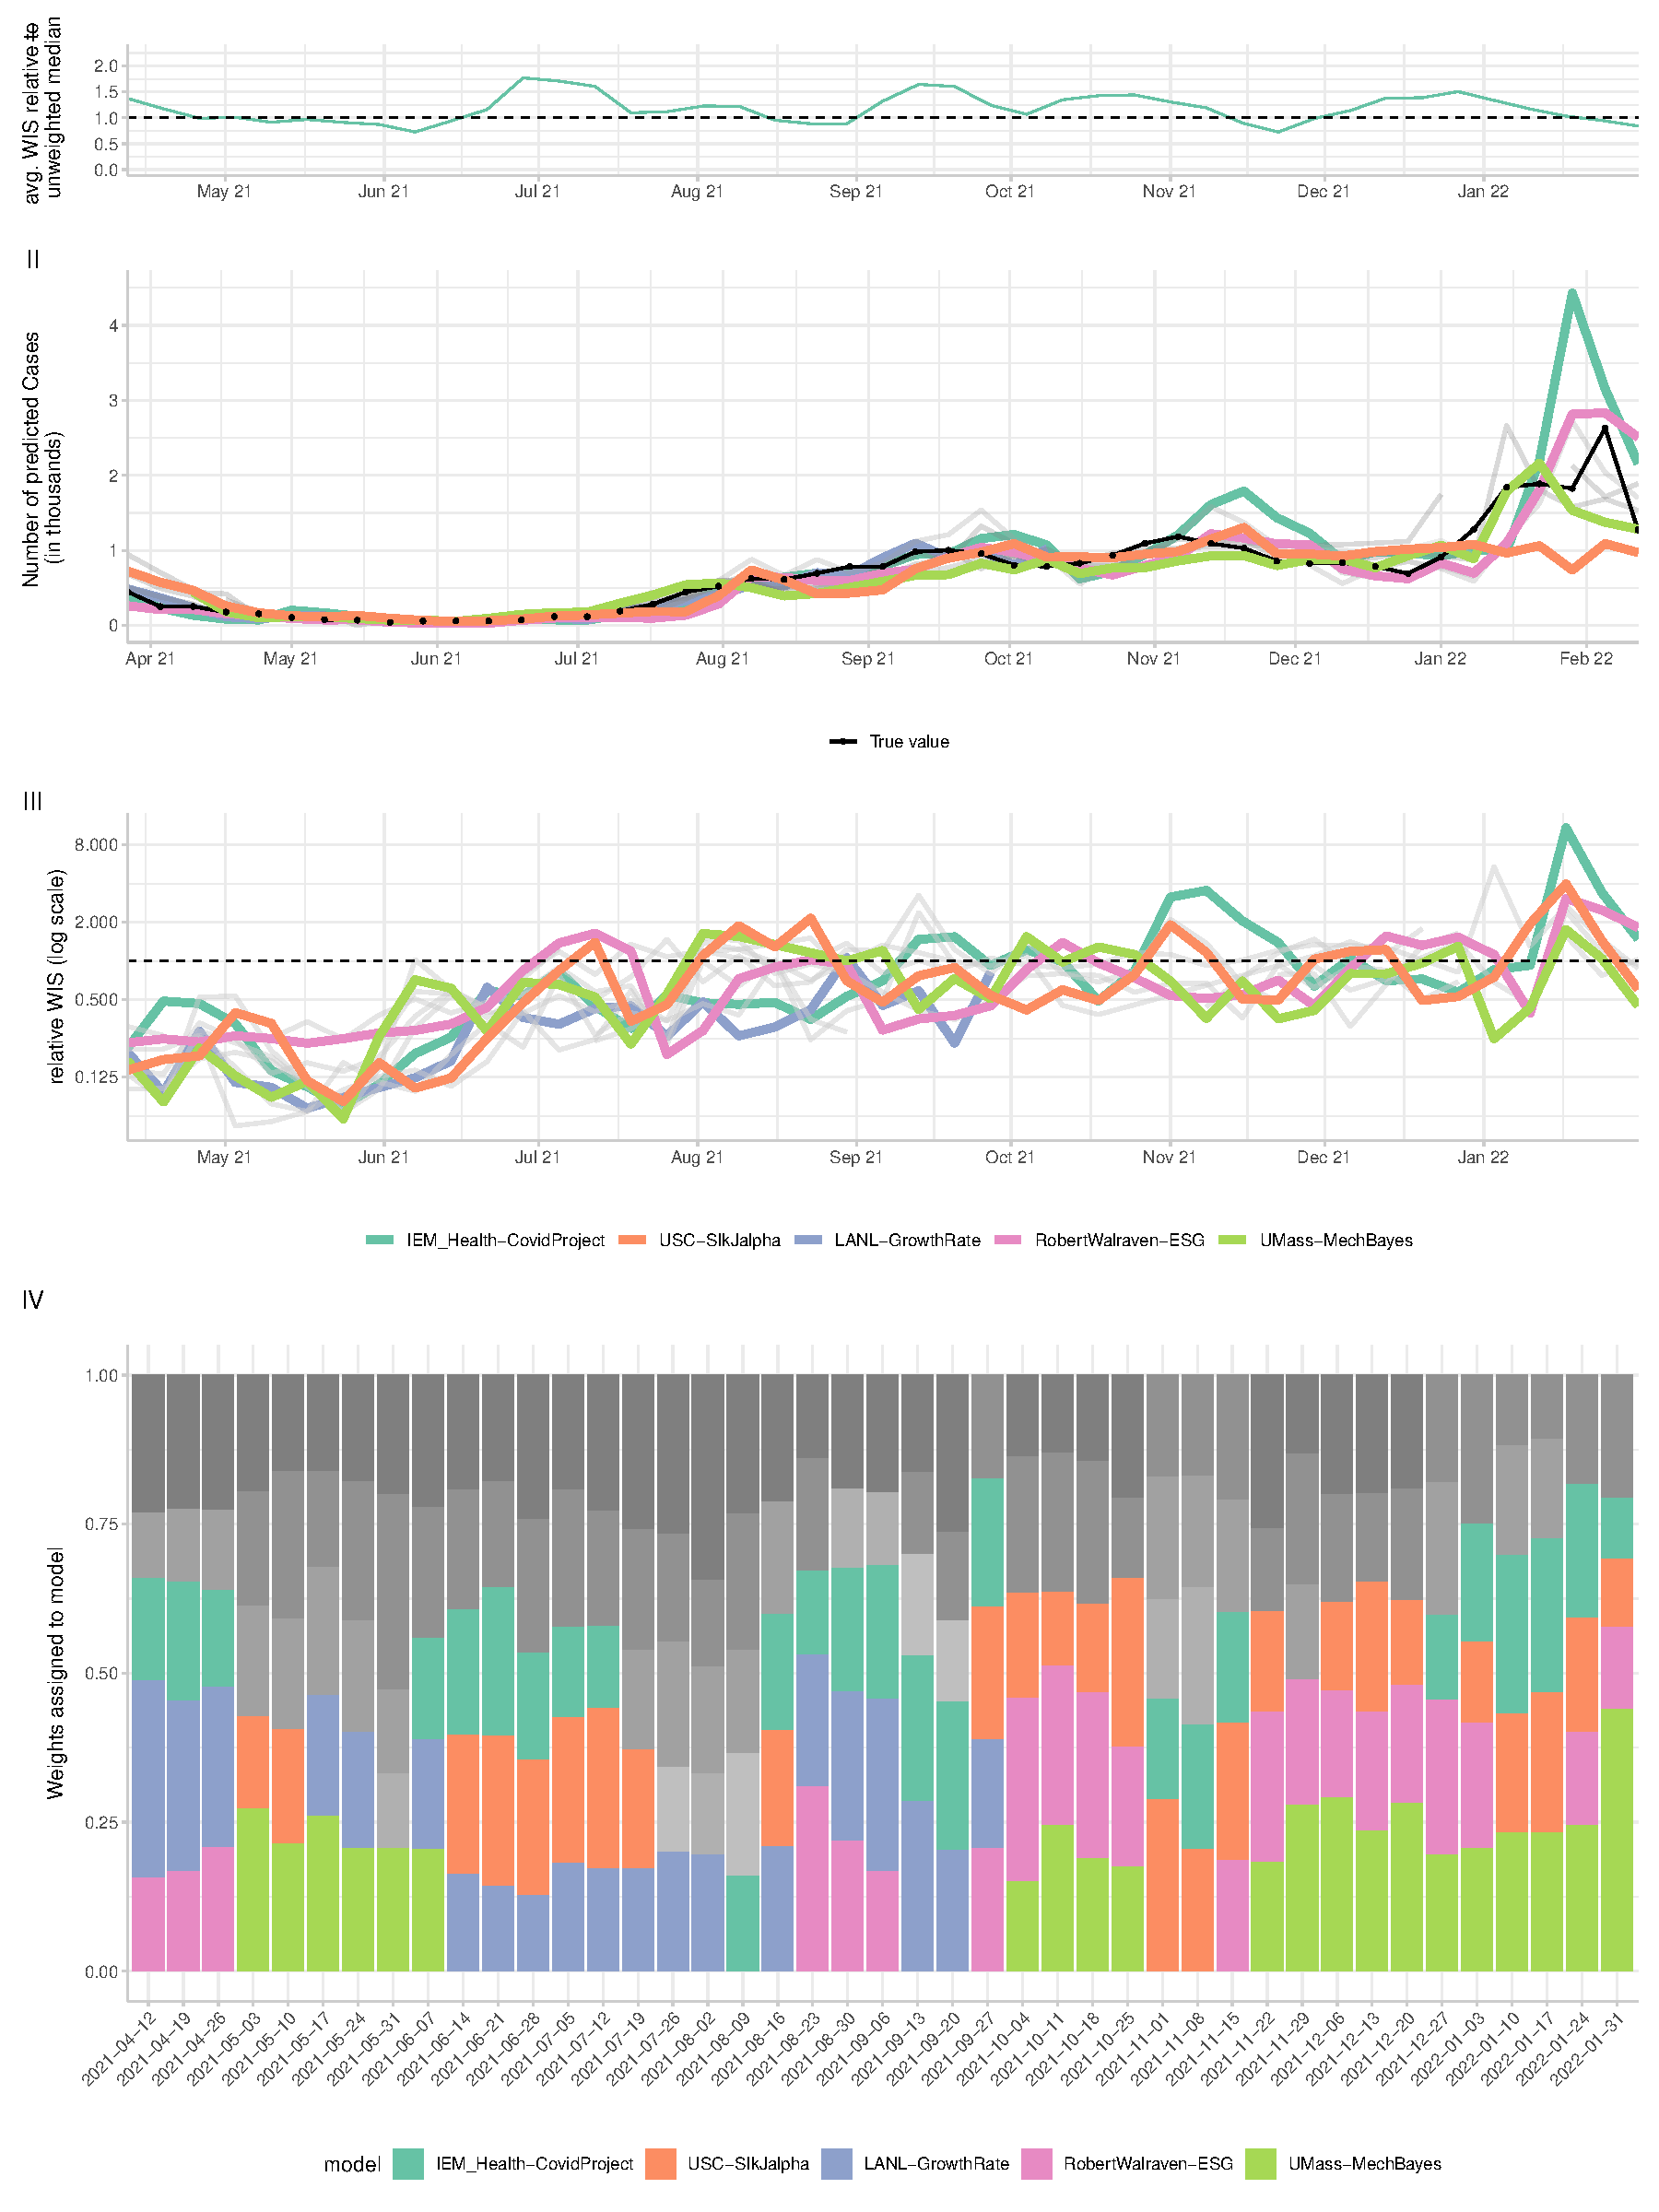
\includegraphics[width = 0.9\textwidth]{../plots/best_performers_weights_gbdeaths}
\caption{\footnotesize{Performance of weekly case forecasts for United Kingdom, for the weighted median selection ensemble based on the five component forecast with best performance, and its component forecasts. Component forecasts are selected and weighted based on their performance in the most recent four weeks. Across all plots, the five models chosen most often for the selection ensemble are highlighted. Panel (I) shows the relative performance of the weighted median selection ensemble based on recent component forecast performance, relative to the benchmark (unweighted median ensemble including all models). Panel (II) shows two week ahead predictions of all component forecasts, as well as the observed values of the series. Panel (III) shows performance of component forecasts over time, in terms of relative WIS. Panel (IV) shows the weekly distribution of weights given to component forecasts. Note that as forecasts are scored by the forecast date, performance measure series lead ahead of the observed incidence series. Furthermore, note that the y-axis of panel (I) was deliberately stretched for compatibility with panel (I) in Figure \ref{fig:bpweights_de}. Plot inspired by \cite{ray_comparing_2022}.}}
\label{fig:bpweights_gbdeaths}
\end{figure}
As we discussed in section \ref{sub:hub_data} and as \cite{ray_comparing_2022} also remark in their discussion of the weighted selection ensemble, Deaths are widely considered the easier target to forecast - one reason for this is that the number of deaths most notably depend on the number of past cases, which is an observable quantity \todos{(cite, e.g. Cramer (2022)?}. On the flip side, if all models show about the same level of skill at predicting future death counts, this also means that it is harder for any model to perform relatively well to another, and therefore harder for the selection method to pick out meaningful better performers. \\
%In fact, when we regard the differences in performance with respect to the two series,  for both the mean and median ensemble, we can see that relative scores for cases are slightly lower than for deaths, which is somewhat contradictory to the aforementioned results in the U.S. Hub. 
%Hence, we would argue  this is likely not due to an inherent difference between the two series: 
As \cite{ray_comparing_2022} argue, the trained method likely works well for forecasting deaths in the U.S. Hub simply because there exist forecasters that have a reliable and consistent track record for forecasting that series, while forecast performance for cases tends to be less stationary for all models. Thus, it is most likely the case that such forecast models simply don't exist for the European Hub and we would argue that, contrary to forecasting cases, the approach seems to fail for forecasting deaths due to overall similar model performance rather than due to failure at critical times. \medskip \\
%In general, we also see that cumulative amount of weights given are never that high.\\
%karlen-pypm not pciked that often Again supporting the point that a model that works well in some locations might not work well in others. (however, availability was also low)\\
%make the argument that and that following structural breaks in the series ()
%During both periods, it would often be beneficial for the ensemble to draw on its entire model base, as there are several other models that receive lower scores E
%%%%%%%%%
%"Trained ensembles that estimated weights based on past performance suffered,as they started to upweight those component forecasters just as their performance dropped. This recurring pattern highlights the challenge that nonstationary component forecaster performance presents for trained ensembles".\\
\begin{figure}
\centering
\includegraphics[width = 0.55\textwidth]{../plots/best_performers_coverage.pdf}
\caption{Assessment of probabilistic calibration of the selection ensemble methods based on recent component forecast performance, relative to the benchmark (equally weighted median ensemble including all models). The upper panel (I) shows central interval coverage of the methods, that is, the proportion of observations falling into the predictive distributions' central prediction intervals. The lower panel (II) shows the difference between the empirical and nominal coverage of the predictive quantiles. Negative (positive) values indicate that less (more) observations fell below a predictive distribution's respective quantile than required. For both panels, the black dashed line corresponds to optimal calibration. For the selection methods, results are based on selecting five best performers for locations with comparatively small model base (Czech Republic, France, United Kingdom) and ten best performers for locations with comparatively large model base (Poland, Germany).}
\label{fig:bpcoverage}
\end{figure}
To assess the methods' probabilistic calibration, we depict coverage of the central prediction intervals as well as one-sided quantile coverage, separately for the different methods, in Figure \ref{fig:bpcoverage}. For coverage of the central prediction intervals, we see in the upper panel that for forecasting cases, all methods are generally overconfident, that is, the predictive distributions' central intervals overall do not cover as many observations as they should, given the respective nominal coverage level. %The difference between the desired coverage level and the empirical coverage level generally increases with the nominal coverage level, which is to be expected. 
The lower panel suggests that this is more of an issue of the upper rather than the lower quantiles, which indicates that the predictive distributions have some downward bias - this is however more the case for the median-based approaches than the mean-based ones, with the weighted median showing most downward bias out of the methods considered. These results are mostly in line with the results of \cite{ray_comparing_2022} for the European Hub, but in contrast to them, we observe that the weighted mean's quantile coverage is more in the line with that of the unweighted mean than that of the weighted median.\\ 
For forecasting deaths, empirical coverage of the central prediction intervals is in general closer to nominal coverage, with only slight under-confidence for the benchmark and the mean-based ensembles. According to panel (II), the weighted selection median is slightly downward biased, with consistently less observations falling below the respective quantiles than required - this is also reflected in its bias measure (which sits at -0.123). In contrast to this, the mean-based approaches show some slighter upward bias,  while the remaining median-based approaches' empirical quantile coverage is more in line with nominal coverage. These results slightly deviate from those of \cite{ray_comparing_2022} for the European Hub - in particular, they find that the weighted median is over-confident, but not biased. \\ %Furthermore, ensembles based on the median as a summary function in general tend to have lower one-sided rates of quantile coverage, with the weighted median being the worst offender. \\
Overall, the methods are thus mostly similar in terms of probabilistic calibration. However, we must note that while the weighted median tended to perform best out of the selection methods considered with respect to relative WIS, it compares less favorably to other methods when assessing calibration, mostly due to its downward bias. \medskip \\% making it a less  option.
For the cases series, we also considered the possibility to focus our analysis (both estimation of weights and the evaluation) on shorter horizons, namely for up to two weeks. This is due to the reason that (as mentioned in section XX) it is a recurrent result across the Hubs that case forecasts tend to be more unreliable for longer horizons and it thus might be desirable to optimize for the one and two week horizons. However, we observed no clear trend that suggested the (weighted) selection method as it was implemented performs better for shorter horizons - see Figure \ref{fig:best_performers_by_horizon} in the Appendix, which displays performance separately by horizon. We see that the selection method seems to work equally well (or rather, poorly) across all four weeks into the future, albeit with some variations. Moreover, considering the estimation of weights, we are already including seven shorter term forecasts vs. three longer term forecasts, so we would not expect any big changes in weights by further restricting this to only horizons one and two weeks ahead. We thus refrained from additionally implementing this strategy. \medskip \\
%Furthermore, one could also conceive of the idea that it might be possible to ``meta-learn'' about models weaknesses, e.g. downweight models that are known to overshoot following initial rises in incidence. However, this approach would need a lot more data as well as require teams to not update their models, which they presumably would want to do given that they know it has a particular issue...\\
%Or, we could use exponential smoothing to estimate scores
% For example, fpr the discussed case for Germany, we had the idea that maybe the method works better at shorter horizons, which would be good, as the interest is generally greater in shorter term horizons anyway. A boxplot that illustrates this can be found in the appendix. ACTUALLY THIS MIGHT BE HUGE!!!!! COULD ARGUE THAT IT'S NOT ONLY JUST LONG HORIZONS THAT ARE THE CULPRIT.\\
Lastly, we briefly mention an interesting lead that emerges when consulting Table \ref{tab:rel_wis_best_performers}. For the case of $k = 5$, we can see that the weighted median mostly performs better than the unweighted median, suggesting that in very small model sets, it could actually be of benefit to weight models by their recent performance, rather than a source of extra noise. Put differently, while it does not emerge as a dominant strategy to actively $reduce$ the set of models, weighting could be applied in situations where only a small number of models is available to begin with. This could be further investigated via other locations in the European Hub, some of which have very small model bases, in a future analysis. \medskip\\
%In theory, one could furthermore devise several different weighting strategies, such as restricting the maximum weights, . 
%Lastly, we want to mention an interesting, while this was not the direct goal of this analysis, we do observe that the weighted median seems to work better than the unweighted median for smaller set of models. This suggests that weighting could actually be used to mitigate against bad performance of a single forecaster in small model sets, rather than a source of extra noise. This could be applied in situations where only a small model base is available to begin with. \\
%Furthermore, the difference between the unweighted and weighted median for small $k$ suggests that in situations where there is only a very small model base available, (while it might not be beneficial to exclude models), it might be good to weight them. \medskip\\
%%%%%%%%%%%%%%%%%%%%%%%%%%%%%%%%%%%%%%%%%%%%%%%%%%%%%%%%%%%%%%%%%%%%%%%%%%%%%%%%%%%%%%
Overall, at least in the sample we are considering, a combination of forecast selection and a weighted median mostly performs okay for forecasting cases but sometimes fails in situations where its component models have drops in performance (mostly by those models overshooting the target), where the method only slowly updates both its component forecasts and their weights. On the one hand, these are the periods that will most drive aggregate scores, and they are also the periods that are of the most interest to decision makers. During these times, it would often be beneficial for the ensemble to draw on its entire model base, to mitigate the effects of those models that overshoot the target. We also note here that if the considered selection procedures actually performed \textit{better} at predicting changes in trends, one might forgive worse performance in other periods, as these moments of increasing case numbers are of particular interest to decision makers. But since the opposite is true and aggregate scores tend to be similar to or worse than the benchmark, with the weighted median additionally showing a tendency for downward bias, we see no reason whatsoever to actually promote its use. \\
An exception could be a case such as the cases series for Poland, where there do seem to exists some models that exhibit better foresight in predicting future case numbers for the method to successfully select and place weight on, but we would still be cautious in recommending such an approach without further investigation into peak behavior in following times. Ultimately, our advice would thus be that decision makers need to consider their respective model set and decide whether such forecasters with good consistent foresight exist.\\ 
Conversely, for forecasting deaths, it seems to be the case that in the European Hub, even when accounting for the fact that models might have higher skill at forecasting some locations more than others, we can't identify component forecasters that perform consistently better.\medskip\\ 
To conclude, we would thus argue that in lieu of the existence of component forecasts that actually perform reliably well, (weighted) selection does not seem to be a viable strategy. Usually, individual model performance is not as consistent as would be needed, again highlighting the benefits of simply using an equally weighted median ensemble that includes all models, which after all has the precise benefit of being able to better mitigate occasional deteriorations in performance from one or some of its member models and not being reliant on measures of past performance.\\
%To conclude, we would thus argue that, at least in the European Hub, it's not inherently Cases vs. Deaths, but simply the presence of good and consistent performers at a given location. For instance, Poland contains models for forecasting cases that exhibit better foresight than others, making the approach more viable.\\
%If asked to generally judge the viability of the (weighted) selection approach with respect to the underlying situation, we would say that our results in conjunction with the results from the U.S. Hub, suggest that the viability of best performers is both a function of the numbers of models to choose from (the added marginal benefit of indiscriminately adding another model to reduce ensemble variability needs to be small) and the existence of some actual consistently good performers. There is also a trade-off between the two: the more consistent the top performers, the smaller the threshold - an example for this is Poland, where $k = 5$ even outperformed $k = 10$. The less consistent, the more models are needed to mitigate any variations in performance. Finally, if model performance is very erratic and past relative good performance is not a reliable predictor for current performance (``models are all the same''), selecting best performers will not work.\\
%Furthermore, we would not suggest it in a situation where the model base is already quite small. \\
%%%%%%%%%%%%%%%%%%%%%%%%%%%%%%%%%%%%%%%%%%%%%%%%%%%%%%
%Thus, while we initially thought that the (weighted) selection method could fail in the European Hub due to the small . would argue that a larger model base would perhaps be helpful, in conjunction with the findings in the US, what we really need are consistent good performers.
%Discuss why it might have worked well in the U.S., but not here (plus reasonings for why it might work well in the US). However, even when investigating the performance over time, suggesting that individual model performance is not as consistent as would be needed and thereby again highlighting the wonders of just using an equally weighted ensemble, which after all has the precise benefit of being able to mitigate occasional and not being reliant on shaky measures of past performance. \\
%To conclude, we thus argue that for model selection to actually make sense, one either needs to be in a space on the model number line where the added marginal benefit of (or conversely, removing one model does not ).\\ \\
%In conclusion, we thus would not recommend in a setting where the model base is already quite small.\\
%Give some coverage plots.\\
%Lastly, one very hypothetical problem with best performers could also be. Consider the case where all model but one slightly overpredict the target, while the last model substantially underpredicts. That model would receive a low score and would never be included in the best performers set, but would be a valuable addition (at least in a median ensemble). However, since we generally run on the assumption that models are not consistently biased in such a way, we disregard this possibility. \\
%%%%%%%%%%%%%%%%%%%%%%%%%%%%%%%%%%%%%%%%%%%%%%%%%%%%%%%%%%%%%%%%%%%%%%%%%%%%%%%%%%%%%%

%%%%%%%%%%%%%%%%%%%%%%%%%%%%%%%%%%%%%%%%%%%%%%%%%%%%%%%%%%%%%%%%%%%%%%%%%%%%%%%%%%%%%%

%%%%%%%%%%%%%%%%%%%%%%%%%%%%%%%%%%%%%%%%%%%%%%%%%%%%%%%%%%%%%%%%%%%%%%%%%%%%%%%%%%%%%%
\subsection{Weighting based on model types} \label{sub:weighting_based_on_model_types}
In this section, we discuss our efforts of implementing weighting schemes that are based on the modeling strategies as discussed previously.\\
As we saw in section \ref{sub:model_types_analysis}, it was not possible to give an overall consistent ranking of model types in the data. One could however then surmise that in specific situations, one general type of modeling philosophy could be better suited than another for giving accurate predictions. We also saw some tentative evidence of this in section \ref{sub:model_types_analysis}: considering Figure \ref{fig:pw_comp_modeltypes_byloc}, we see that in terms of the WIS, it would have for instance been beneficial for most locations to rely more heavily on the statistical models within the set during ``Period 5'', that is, the period that observed the most growth. (perhaps better: downweight semi-mech. models and \\
The idea of selecting component forecasts for an ensemble based on their model type does have some precedence in the literature. In their analysis of the deaths series in the U.S. Hub, \cite{taylor_combining_2021} identified that for states that had relatively low overall mortality compared with others, ensembles that exclusively consisted of compartmental models gave the most accurate forecasts, while the same strategy gave similar performance for states with medium mortality and worsened performance for states with high mortality, compared to an ensemble including all types of models. Apart from this, we are unaware of any studies attempting to base ensemble composition or weights on model types.\\
We thought about implementing a similar strategy as the one by \cite{taylor_combining_2021}, but given the small number of locations in our set, which furthermore show similar levels of incidence when accounting for population size, we did not think this to a viable idea. We instead originally considered the idea of categorizing phases of the pandemic (based e.g. on some notion of ``stable'', ``upswing'', ``downswing''), as we also believed that differences between model types would most likely show along these lines (e.g. statistical models might be better at modeling exponential growth of cases) - we however also ultimately found that any such categorization would be arbitrary to a non-negligible degree, since most series exhibited intermittent periods of growth even during the summer months (which did see lower incidence in general).\\
Again, we want to mimic the real-time situation as closely as possible. While we did observe that on average, the group of semi-mechanistic models overshot during period 5 and thus critically drove scores and it would thus likely be beneficial (in terms of the WIS) to exclude these models, implementing this type of ensemble retroactively would rely too much on implementing hindsight knowledge.\\
Hence, given our findings that selecting and/or weighting \textit{individual} component forecasts based on recent performance measures does not seem to reliably improve the ensemble, the question arose whether it might be possible to leverage differences in recent performance at the level of model types, rather than at the individual model level. We thus decided to implement a strategy that estimated weights based on model types.\\
Before we give the implementation and our results, we want to discuss some reasons why we thought this could and could not work. As already mentioned, we did observe some tentative evidence that some model types performed better than others during some periods, and we wanted to test whether an automatic weighting scheme might be able to pick up on this. Moreover, grouping models and thereby weighting at the level of model types rather than individual models has the advantage of being able to use all models, even if they newly enter into the Hub and no individual record of performance is available yet. Furthermore, due to models dropping in and out of predicting, there sometimes exist gaps for each model, so we often lack a consistent record of recent performance to base weight estimation on. On the level of model types, we don't have these gaps.\footnote{except for a brief section at the beginning of the study period where we have no statistical models for UK, France and CZ for forecasting cases.} Lastly, this procedure presumably removes some variability from the practice of estimating weights: if a single model has some fluctuations in performance, this will impact a grouped score less than individual scores.\\
However, while model types do share a common approach to modeling, they are of course not a monolith and characteristics other than their categorization within these groups can dominate their performance. The categorization might thus not be meaningful enough. But most of all, this strategy could presumably suffer from the same problem as that which we discussed in the previous section: performance could not be stationary enough to allow good estimation of weights and a weighted ensemble might thus be too slow at adapting to changes in trends. \\
We devised two different and unique methods to test this strategy out: for the first, we decided to use the inverse score weighting approach as used in the previous section, but computed the average score in the respective window at the level of model types rather than single models. From this, we (as previously) calculated a weight for each model type, which we then divided by the number of models available for it and assigned the resulting weight to the respective member models. In other words, this amounts to weighting the groups unequally, but giving each component forecast within each group equal weight. Differently to before, we decided to use an exponential weighting scheme to calculate the recent score of model types, as we hoped that this would let the method adapt faster to changes in performance, while simultaneously still including faraway scores so as not to increase the variance of the estimation too much, albeit to a lesser degree.\\
\begin{table}[t]
\centering
\begin{tabular}{llcccccc}
  \hline
 & Method & Average & Czech R. & Germany & France & U.K. & Poland \\ 
  \hline
\multirow{3}{*}{\rotatebox[origin=c]{90}{Cases}}& Inv. score w. median & 0.996 & 1.021 & 1.187 & 0.991 & 0.895 & 0.995 \\[0.15em] 
& QRA & 1.268 & 1.239 & 1.123 & 1.177 & 1.488 & 1.197 \\[0.15em] 
& QRA - adj. weights & 1.159 & 1.165 & 1.038 & 1.118 & 1.287 & 1.121 \\[0.99em]
\multirow{3}{*}{\rotatebox[origin=c]{90}{Deaths}}& Inv. score w. median & 1.141 & 1.059 & 1.176 & 0.856 & 1.047 & 1.404 \\[0.15em]  
& QRA & 1.318 & 1.124 & 1.234 & 1.085 & 1.172 & 1.707 \\[0.15em]  
& QRA - adj. weights & 1.169 & 0.948 & 1.096 & 1.191 & 1.021 & 1.388 \\ 
   \hline
\end{tabular}
\caption{Table showing the relative performance of the methods compared to the benchmark (an equally weighted median based on the same models) \todos{stratify this by horizon?}}
\label{tab:mt_weights}
\end{table}
%between bias and variance when estimating recent performance of a model: using only a few recent observations to build average performance gives low bias, but also increases variance due to possible random fluctuations in model performance. Exponential weighting of the scoring history gives more weight to recent scores, but also includes faraway scores to a lesser degree so as to reduce the variance of the estimation. Mainly, we did this, while nevertheless not wholly excluding scores that are farer away.\\ 
As a second strategy, we first built an equally weighted median ensembles from each of the model types, thus in effect giving three smaller ensemble models. For these, we then calculated QRA weights as detailed in section XX. We however noticed that the resulting weights could be quite variable and also sometimes tended toward the extreme ends (at certain weeks exclusively giving all weight to one of the ensembles). Furthermore, we thought it wiser to additionally account for the differing availability of models for the respective model types over time amount of models within each group, we additionally decided to implement a simple adjustment strategy that amounts to balancing the weights equally between those that the QRA algorithm calculated and those that are purely based on the size of the respective ensembles.\\
Since we want to focus on the general viability of the approach and in section \ref{sub:model_types_analysis} we mainly considered the three dominant model types within the Hub, we here use the equally weighted median ensemble including only models of those types in the analysis - in practice, this thus excludes the expert judgment based model as well as the two agent-based models for Poland. We do this to see whether a weighting via categorization is \textit{in principle} fruitful or possible and want to remove the confounding factor of ensemble size. At the end of the section, we however also compare against the true benchmark for full disclosure. \\ 
The results, again stratified by location and target type, are shown in \ref{tab:mt_weights}. Similarly to before, we observe no clear general benefit of any method. QRA is the worst, although it also . Weighting at the level of model types is hence not a viable alternative to 
%For this section, we base comparison on the equally weighted median based on the same set of models. We do this to see whether a weighting via categorization is in theory fruitful or possible. The full comparison will be in the overall assessment in subsection ...\\
%To summairse: the hope is that if there are periods of the pandemic where a certain model type has an edge over others, this system will recognize this and weight accordingly. \\
%%%%%%%%%%%%%%%%%%%%%%%%%%%%%%%%%%%%%%%%%%%%%%%%%%%%%%%%
% while \citep{bracher_pre-registered_2021} have identified that following changes in trends, statistical models perform more poorly, likely because they first have to observe the changing trend in the data from which they extrapolate.\\
%As stated before, weighting might not be the best idea. However, in practice there might be correlations of forecast performance - in sofar as this happens at the level of model types, one might be able to exploit that.\\
%Schreib irgendwas darüber warum vielleicht ein Modelltyp einem anderen theoretisch überlegen sein könnte in bestimmten Phasen. Statistical exponential,... This might be hard to implement explicitly, but automatic weighting might work.\\
%To echo this, during our investigation of model types in section ??, we also observed that , although these did not necessarily follow any strict rules as outlined above. Nevertheless, if we for instance regard Figure ??, we can most prominently see for e.g. France that model type performance varies by period, with one type dominating the other at certain times. It would thus have been preferable to use only one type of model. Thus, we want to investigate whether these relative performance differences can be picked up by an automatic weighting scheme. \\
%\cite{taylor_combining_2021} conjecture that during periods of low incidence, mechanistic models should perform better than statistical ones. This is due to the fact that random statistical fluctuations can still occur, but statistical models might, somehow, latch on to these too eagerly and proceed to forecast exponential growth where there is none.\\
%Two problems with inverse score weighting that shrinkage towards equal weights can fix: \\
%- can overweights on e.g. statistical (which could be problematic because past predictive power is of course not a perfect; overshoot after exponential growth)
%- we don't optimize for performance at all. Linear combination of two weights is of course not super flexible, but it gives at least a small dial for actual performance optimization to happen. \\ 
%And anyway, results from previous section did not show robust trends. Instead, the idea is to use recent performance of the model types to weight them differently in an ensemble. As mentioned, due to models dropping in and out of predicting, there are substantial gaps for each model and thus not yielding a consistent record of recent performance that one could use to weight on. On the level of model types, we don't have these gaps. The idea thus is to first build an ensemble for each model type in the data and then to weight these respective ensembles with respect to their recent performance. The hope is that if there are periods of the pandemic where a certain model type has an edge over others, this system will recognize this and weight the models accordingly. \\
%%%%%%%%%%%%%%%%%%%%%%%%
%Semi-rem: Thus, even bad models will provide some benefit\\
\subsection{Overall}
Is mean or median better in period 5? Would expect median to be more robust in times of stark growth.
\section{Contributions}
``We have used the WIS and probabilistic calibration to measure the extent to which forecasts
are consistent with the eventually observed data. These summaries of performance are commonly
used and provide useful insights into forecast performance, but it is worth noting that they do
not necessarily reflect the utility of the forecasts for every particular decision-making context.
Aggregated summaries of performance, such as overall quantile coverage rates could obscure finerscale
details —for instance, a method with good coverage rates on average could have high coverage
at times that are relatively unimportant and low coverage when it matters. Additionally, for some
public health decision-making purposes, one or another aspect of a forecast may be more important;
for example, some users may prioritize accurate assessments about when a new wave may begin,
but other users may find accurate forecasts of peak intensity to be more important. Our evaluation
metrics do not necessarily reflect the particular needs of those specific end users, and it is possible
that different ensemble methods would be more or less appropriate to generate forecasts that serve
different purposes.'' \citep{ray_comparing_2022}.
A lot of work has been done on the US forecast hub. We wanted to investigate whether improvement gains could be made in a setting with a smaller model base and less consistent submissions. While Sherratt showed that weighting did not work, we wanted to know... Ultimately, we came to the same conclusion that has been highlighted before in other studies: past performance is not a reliable predictor for current performance, neither at the individual model level or at the level of model groups/types. \\
While we saw in section \ref{sub:model_types_analysis} that a retrospective analysis showed that there were some systematic differences between model types, when trying to mimic a real-time setting and simply relying on measures of recent past performance on how to weight model types, we saw that it was not possible to consistently make use of this when simulating a real-time setting.  \\
Thus, even though we, contrary to the U.S. Hub approach, addressed both the lack in flexibility and the number of models , thereby ruling these out as the sole causes of the issue.\\\\
Perhaps an overarching meta result from our study is that locations in the European Hub wildly differ and what may. It might sometimes be possible to find methods that seem to work in the aggregate, but that end up showing wildly different results when looking at locations separately. Overall, we would argue that the countries are too heterogeneous to establish a central modeling strategy.\\
The fundamental problem with the best performers approach is thus that it reduces the model set based on past performance, which given the nonstationarity of model performance, is not a reliable predictor for future performance - once a model is in there, it will be given positive weight - if it then performs poorly, this will have a bigger effect on the ensemble than if the ensemble instead drew from its entire model base.\\
Lastly, we again want to caveat that our method of evaluation is very descriptive and frankly too high dimensional. Ideally, one would want to employ a model to consolidate dimensions, but we sadly can't do that. \\
Overall, we think that we have demonstrated that the countries in the set are simply too heterogeneous to warrant indiscriminate statements. Our recommendation would be to always regard the specific situation and wherever resources and or the dominant models aren't available, to rely on the simple median ensemble instead.\\
One could also conceive a strategy where one adaptively changes weights after .\\
\begin{figure}
\centering
\includegraphics[width = 0.95\textwidth]{plot_placeholder/perform_ensemble_ovrtime.png}
\caption{From \cite{ray_ensemble_2020}. Plot different ensemble techniques over time}
\
\end{figure}
\bibliography{references}
\bibliographystyle{plainnat}

\appendix
\input{tables/gamma_results_nmod4_sens}

\begin{figure}
\centering
\includegraphics[width = 0.95\textwidth]{../plots/appendix/gamma_reg_random_effects_nmod8.pdf}
\caption{Best performers, by horizon}
\label{fig:replot_nmod8}
\end{figure}

\begin{figure}
\centering
\includegraphics[width = 0.95\textwidth]{../plots/appendix/best_performers_boxplot2.pdf}
\caption{Best performers, by horizon}
\label{fig:best_performers_by_horizon}
\end{figure}
\end{document}

